\documentclass{article}
\usepackage{course_work} % Load your custom package!

\title{
    
\includegraphics[scale=0.2]{Images/cam_logo_bw.png}\\ % Use a relative path!
    \vspace{0.5cm}
    S2: Advanced Statistical Methods
}
\author{Yuchen Mao (ym429)}
\affil{Department of Physics, University of Cambridge}
\date{\today}
\usepackage{array}
\usepackage{siunitx}
\usepackage{booktabs}
\usepackage{amsmath}
\usepackage[T1]{fontenc}
\usepackage[utf8]{inputenc}
\usepackage{makecell} % Required for line breaks within cells
\usepackage{tablefootnote}

\begin{document}
\setstretch{1}
\maketitle
\noindent\textbf{Word count: 2998}
\setpagefooter{2998}{Yuchen Mao} % Set the footer *after* \begin{document}
\tableofcontents
\setstretch{1.1}

\newpage


\section{Introduction}
\label{sec:introduction}

This report describes the fine-tuning of the \texttt{Qwen-2.5-0.5B-Instruct} large language model (LLM) — originally trained for natural language tasks — for forecasting predator-prey time series. This adaptation was undertaken within a challenging constraint: a strict computational budget of $1 \times 10^{17}$ Floating Point Operations (FLOPS) covering all experimental stages. To achieve this, we employed the LLMTime preprocessing scheme \cite{gruver2024largelanguagemodelszeroshot} for efficient numerical sequence representation and Low-Rank Adaptation (LoRA) \cite{hu2021loralowrankadaptationlarge} for parameter-efficient fine-tuning. Through systematic experimentation, including hyper-parameter optimization guided by careful FLOPS calculation and planning, we demonstrate a significant improvement in the model's forecasting accuracy compared to its untrained performance. Overall, this work documents the methodology, experimental progression, key findings, and showcased the overall effectiveness of adapting a tiny LLM for this quantitative task under significant resource constraints. The code is available at our \href{https://gitlab.developers.cam.ac.uk/phy/data-intensive-science-mphil/assessments/m2_coursework/ym429}{GitLab repository}, with a tutorial and documentation at \href{https://yuchen20.github.io/M2-Coursework/}{GitHub Pages}.

\section{Dataset}
\label{sec:dataset}

This study uses a dataset of 1000 distinct Lotka-Volterra systems, simulating predator-prey population dynamics. Each system is a time series data of 100 time-steps, with both predator and prey population levels. Examples are visualized in Figure \ref{fig:dataset_examples}. The primary task is to fine-tune the pre-trained \texttt{Qwen-2.5-0.5B-Instruct} model using this dataset, such that the model is able to learn the underlying temporal patterns governing these interactions and accurately forecast future population levels based on sequences of past observations.


\begin{figure}[!htbp] % Use positioning options like htbp
    \centering % Center the entire grid

    \begin{subfigure}[b]{0.4\linewidth} % [b] aligns subfigure bottoms
        \centering
        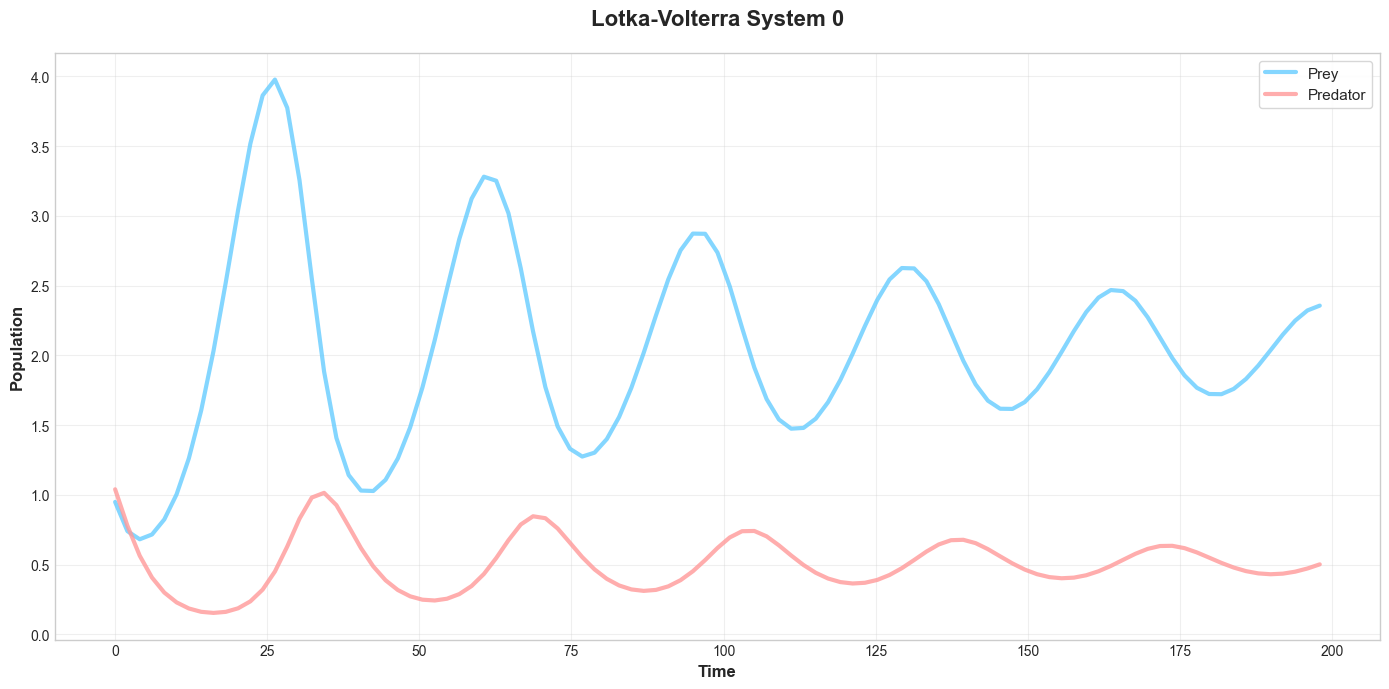
\includegraphics[width=\linewidth]{M2 Course Work//Images/dataset_vis_timeseries_0.png}
        \caption{Time series plot for System 0.}
        \label{fig:ts_0}
    \end{subfigure}
    \hfill % Adds horizontal space between the subfigures
    \begin{subfigure}[b]{0.4\linewidth}
        \centering
        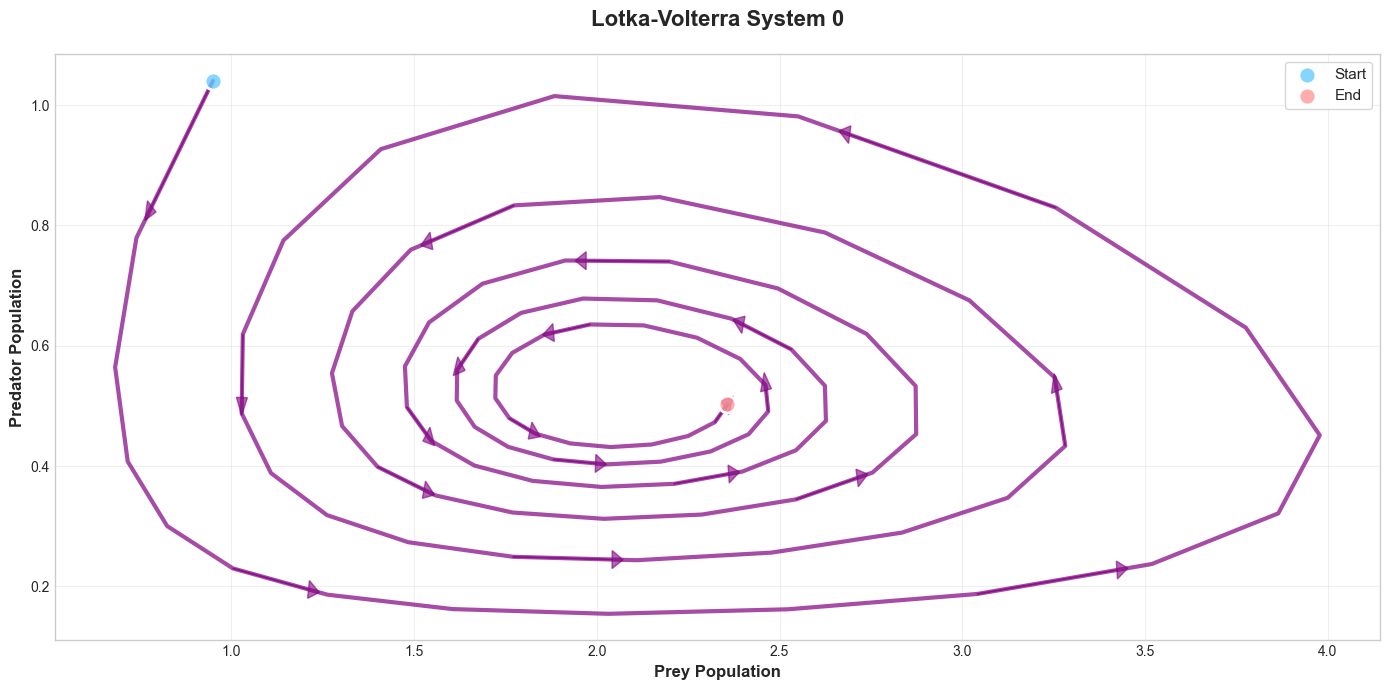
\includegraphics[width=\linewidth]{M2 Course Work//Images/dataset_vis_phase_0.png}
        \caption{Phase portrait for System 0.}
        \label{fig:phase_0}
    \end{subfigure}

    \vspace{0.2cm} % Adds a small vertical space between rows

    \begin{subfigure}[b]{0.4\linewidth}
        \centering
        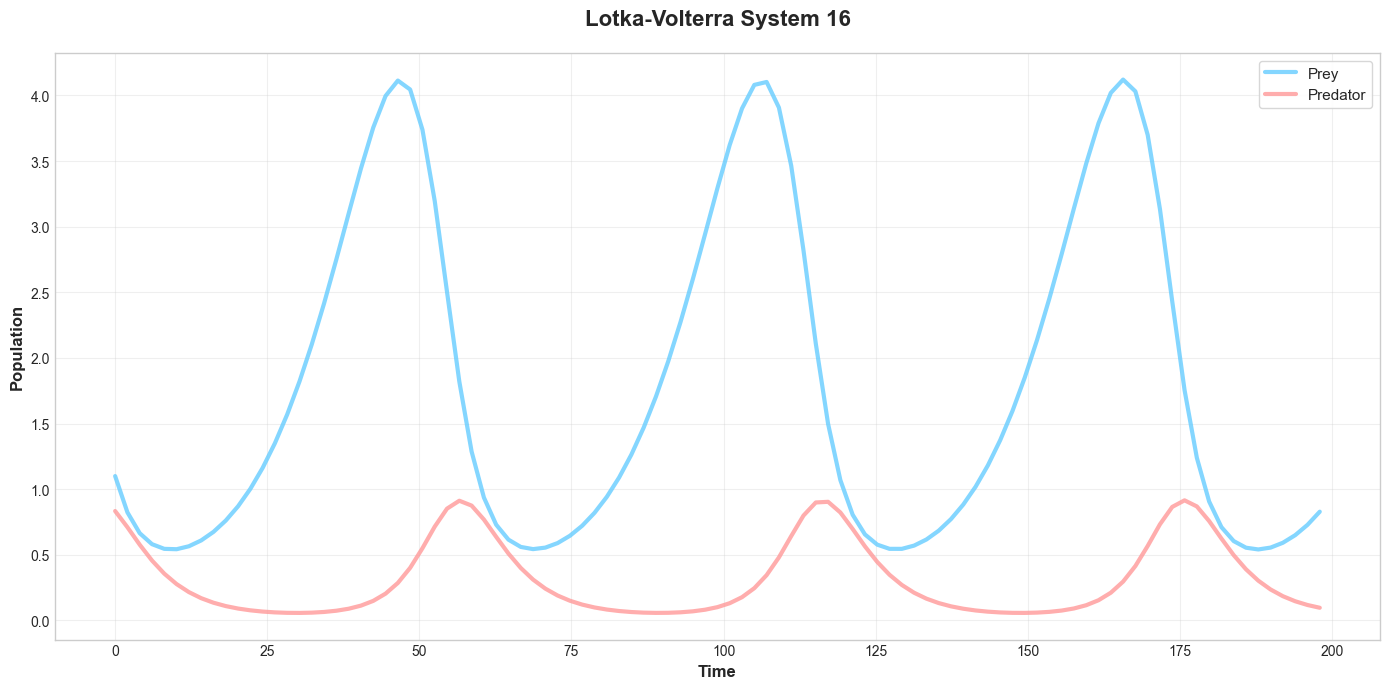
\includegraphics[width=\linewidth]{M2 Course Work//Images/dataset_vis_timeseries_16.png}
        \caption{Time series plot for System 16.}
        \label{fig:ts_16}
    \end{subfigure}
    \hfill % Adds horizontal space
    \begin{subfigure}[b]{0.4\linewidth}
        \centering
        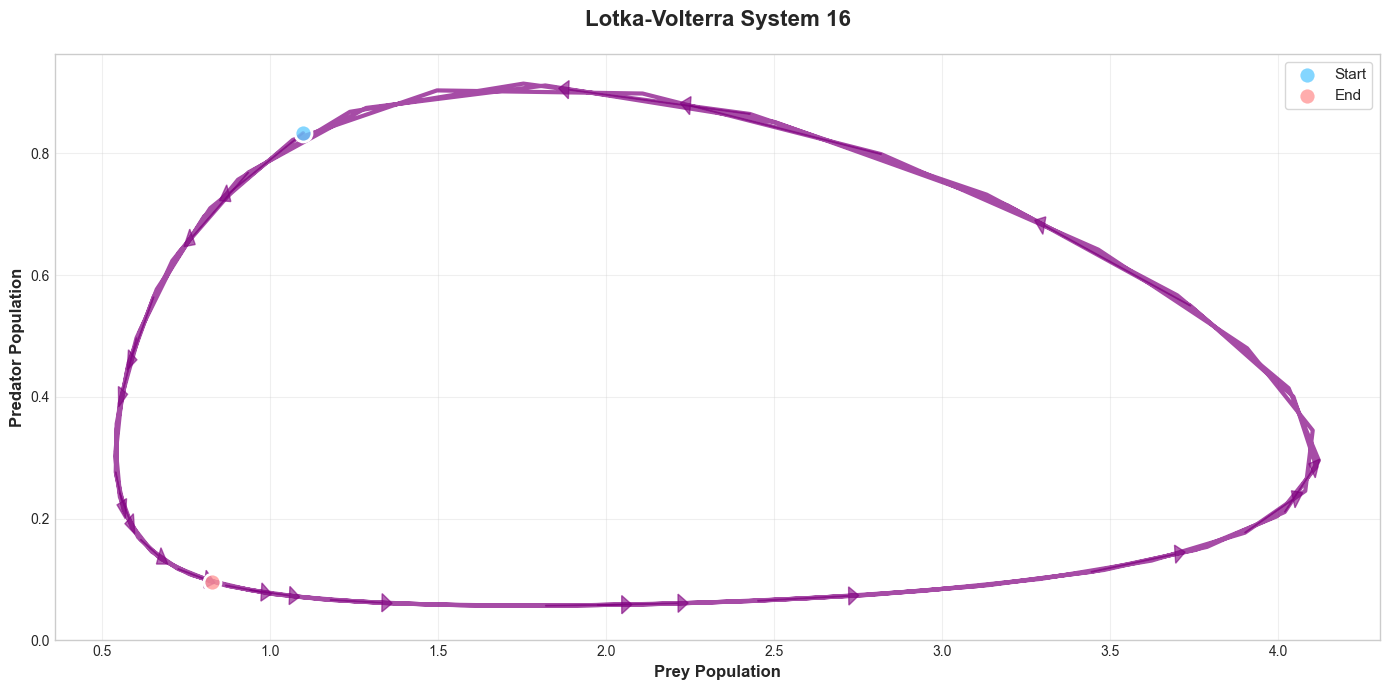
\includegraphics[width=\linewidth]{M2 Course Work//Images/dataset_vis_phase_16.png}
        \caption{Phase portrait for System 16.}
        \label{fig:phase_16}
    \end{subfigure}

    \caption{Visualization of predator-prey dynamics for two example systems (0 and 16) from the dataset. Subfigures (a) and (c) show population levels (Prey in blue, Predator in orange) over 100 time steps. Subfigures (b) and (d) display the corresponding phase plots, illustrating the cyclical relationship between prey and predator populations.}
    \label{fig:dataset_examples} % Unique label for the entire figure
\end{figure}


\section{LLMTime Preprocessor}
\label{sec:preprocessing}

Fine-tuning LLMs like \texttt{Qwen-2.5-0.5B-instruct} on numerical time-series data presents a challenge: standard tokenization schemes are inefficient for floating-point numbers. For instance, Qwen's tokenizer represent $0.12345$ as a sequence of individual digit and punctuation tokens $[0, ., 1, 2, 3, 4, 5]$, inflating sequence length and computational cost. To address this, we implemented the preprocessing method proposed by LLMTime \cite{gruver2024largelanguagemodelszeroshot}, designed to create a more compact and LLM-friendly representation.

\begin{figure}[!h]
    \centering
    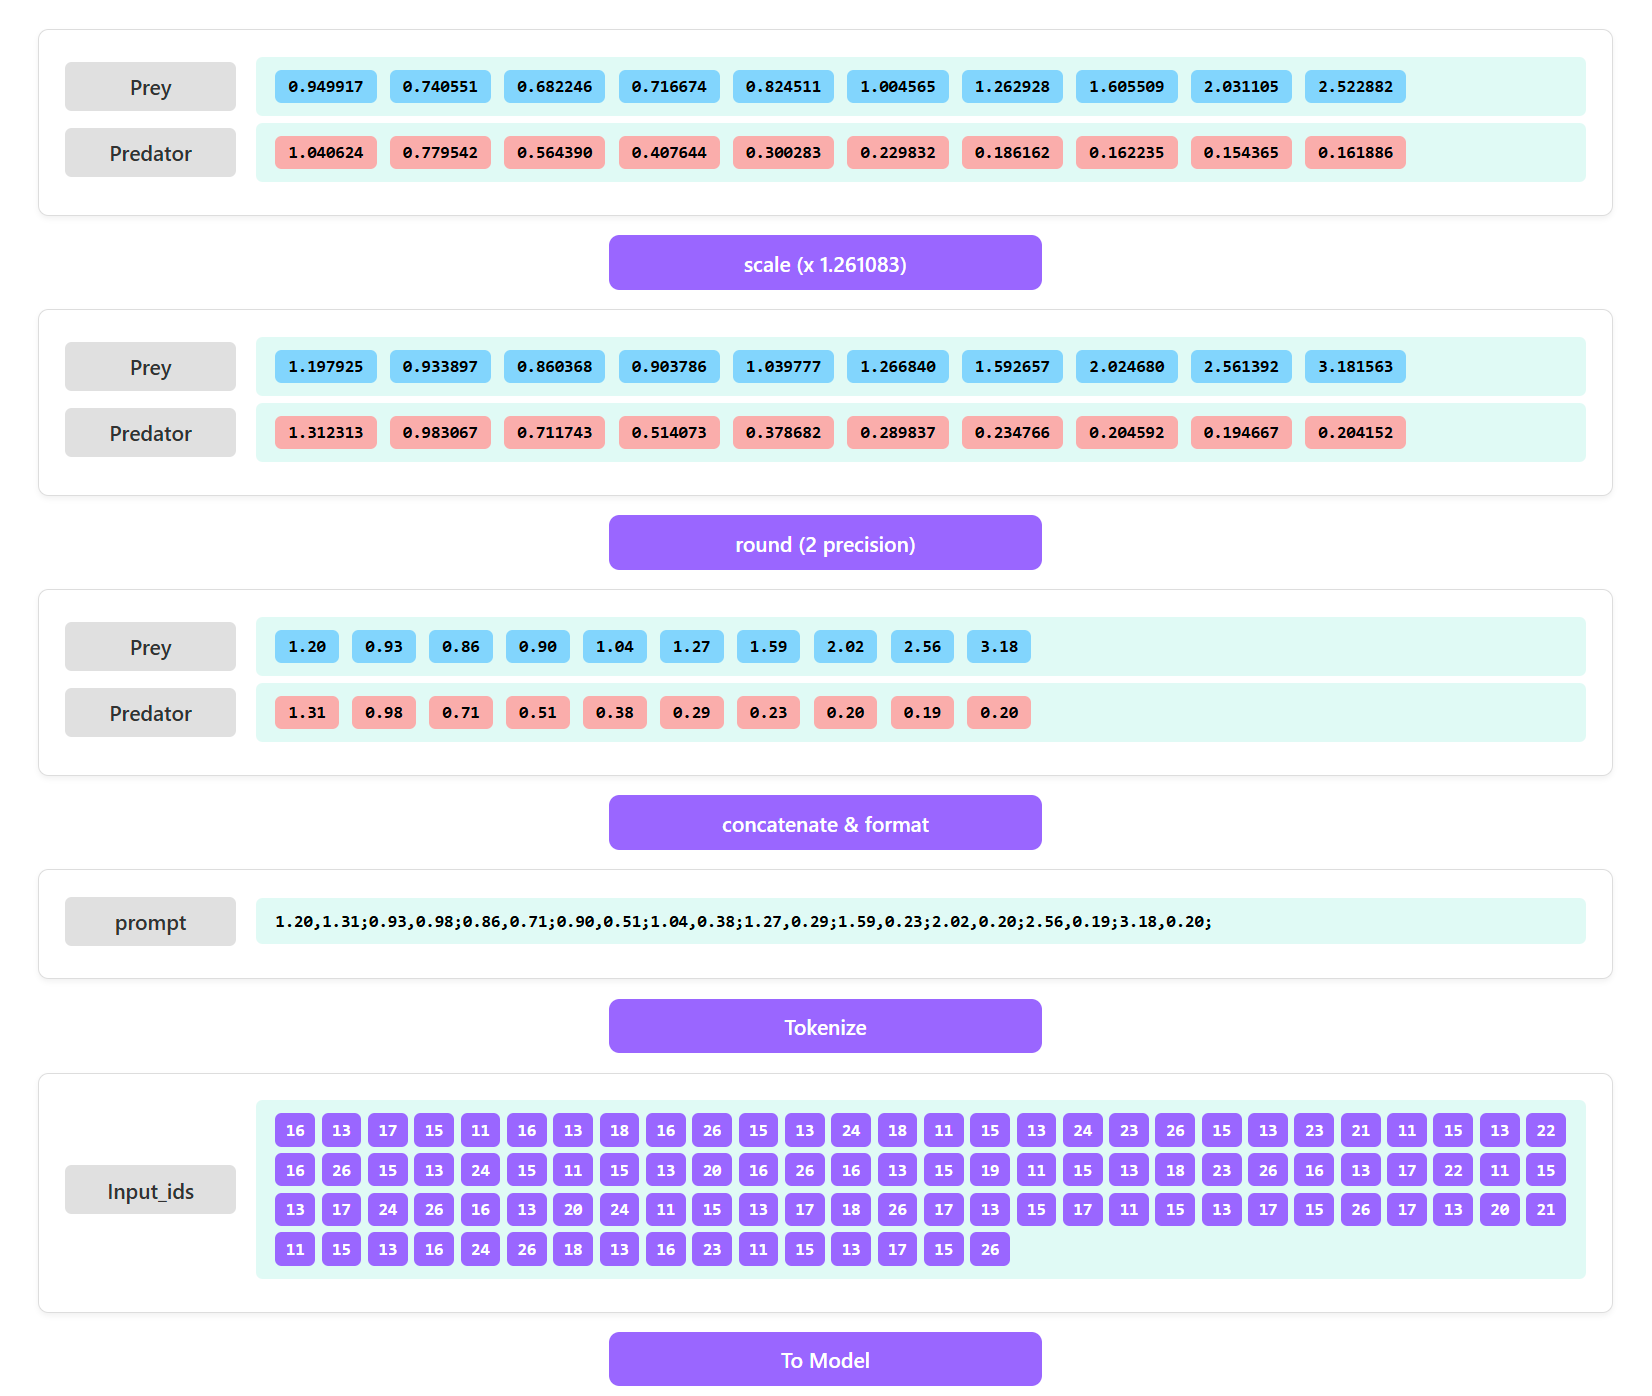
\includegraphics[width=\linewidth]{M2 Course Work/Images/preprocess_vis.png}
    \caption{Visual workflow of the LLMTime preprocessing: raw data undergoes scaling (to [0, 10]), rounding (2 decimal places), and formatting into a structured string suitable for LLM input.}
    \label{fig:preprocessing_visual_workflow}
\end{figure}

The process, illustrated in Figure \ref{fig:preprocessing_visual_workflow}, involves three main steps:
\begin{zenumerate}
    \item \textbf{Scaling}: Values are scaled to map the majority (up to the 99.7th percentile) into the range $[0, 10]$ using a calculated scaling factor (Equation \ref{eq:scaling_factor}). While this aims to achieve a compact representation, it unfortunately imposes an unnatural upper limit on the range of predictable values, as discussed further in Section \ref{sec:discussion}.
    \begin{equation}
        \text{scaler} = \frac{10}{\text{percentile}_{99.7}(\text{data})}.
        \label{eq:scaling_factor}
    \end{equation}
    \item \textbf{Rounding}: Scaled values are rounded to two decimal places (e.g., \texttt{X.XX}) to standardize the format and reduce token usage. Note that this operation results in information loss, which will be assessed later in this section.
    \item \textbf{Formatting}: The processed numerical pairs (prey, predator) are formatted into a single string. Values at the same timestamp are comma-separated, and different timestamps are semicolon-separated (e.g., $p_t, h_t ; p_{t+1}, h_{t+1} ; ...$). This preserves temporal structure while being easily tokenizable.
\end{zenumerate}





To quantify the impact of scaling and rounding, a round-trip evaluation (scaling, rounding, formatting and decoded back to time-series data) was performed. As shown in Table \ref{tab:round_trip_test}, the Mean Absolute Error (MAE) between the original and recovered values is only $0.002167$. This confirms that the preprocessing introduces minimal information loss while significantly reducing sequence length, enabling more efficient training and inference. Implementation details can be found in preprocessor python file\footnote{\href{https://gitlab.developers.cam.ac.uk/phy/data-intensive-science-mphil/assessments/m2_coursework/ym429/-/blob/main/src/preprocessor.py?ref_type=heads}{see \texttt{src/preprocessor.py} file}} and the accompanying notebook\footnote{\href{https://gitlab.developers.cam.ac.uk/phy/data-intensive-science-mphil/assessments/m2_coursework/ym429/-/blob/main/notebooks/1_dataset_preprocess.ipynb?ref_type=heads}{see \texttt{notebooks/1\_dataset\_preprocess.ipynb} file}} for tutorial.



\begin{table}[!thbp]
\renewcommand{\arraystretch}{1.4}
\centering
\caption{Round-trip evaluation assessing information loss from the LLMTime preprocessing method (scaling, rounding, formatting and decoded back to time-series data). The Mean Absolute Error between the original and recovered time-series data is $0.002167$. This minimal difference between original and recovered values hints that the preprocessing preserves essential signal characteristics despite significant data condensation required for Large Language Model compatibility.}
\label{tab:round_trip_test}
\footnotesize
\begin{minipage}{0.48\textwidth}
    \centering
    \caption*{\textbf{Prey Values}}
    \begin{tabular}{ccccc}
        \toprule
        \textbf{Time} \qquad & \textbf{Original} \qquad & \textbf{Processed} \qquad & \textbf{Recovered} \qquad & \textbf{Difference} \\
        \midrule
        0 & 0.949917 & 1.20 & 0.951563 & 0.001646 \\
        1 & 0.740551 & 0.93 & 0.737461 & -0.003090 \\
        2 & 0.682246 & 0.86 & 0.681954 & -0.000292 \\
        3 & 0.716674 & 0.90 & 0.713672 & -0.003002 \\
        4 & 0.824511 & 1.04 & 0.824688 & 0.000177 \\
        5 & 1.004565 & 1.27 & 1.007071 & 0.002506 \\
        6 & 1.262928 & 1.59 & 1.260821 & -0.002107 \\
        7 & 1.605509 & 2.02 & 1.601798 & -0.003711 \\
        8 & 2.031105 & 2.56 & 2.030001 & -0.001104 \\
        9 & 2.522882 & 3.18 & 2.521642 & -0.001240 \\
        \bottomrule
    \end{tabular}
\end{minipage}%
\hfill%
\begin{minipage}{0.48\textwidth}
    \centering
    \caption*{\textbf{Predator Values}}
    \begin{tabular}{ccccc}
        \toprule
        \textbf{Time} \qquad & \textbf{Original} \qquad & \textbf{Processed} \qquad & \textbf{Recovered} \qquad & \textbf{Difference} \\
        \midrule
        0 & 1.040624 & 1.31 & 1.038790 & -0.001834 \\
        1 & 0.779542 & 0.98 & 0.777110 & -0.002432 \\
        2 & 0.564390 & 0.71 & 0.563008 & -0.001382 \\
        3 & 0.407644 & 0.51 & 0.404414 & -0.003230 \\
        4 & 0.300283 & 0.38 & 0.301328 & 0.001045 \\
        5 & 0.229832 & 0.29 & 0.229961 & 0.000129 \\
        6 & 0.186162 & 0.23 & 0.182383 & -0.003779 \\
        7 & 0.162235 & 0.20 & 0.158594 & -0.003642 \\
        8 & 0.154365 & 0.19 & 0.150664 & -0.003700 \\
        9 & 0.161886 & 0.20 & 0.158594 & -0.003292 \\
        \bottomrule
    \end{tabular}
\end{minipage}
\end{table}






\section{FLOPS Calculation}
\label{sec:flops}

Training modern LLMs requires substantial computational resources. However, due to the strict budget of $1 \times 10^{17}$ FLOPS imposed by this coursework for all reported experiments, careful planning and efficient experimentation are required. This section details the algorithm used to estimate the FLOPS cost for fine-tuning the \texttt{Qwen-2.5-0.5B-Instruct} model with LoRA, allowing us to manage experiments within the budget.

\subsection{Model Components and Assumptions}



\begin{figure}[!htbp]
    \centering
    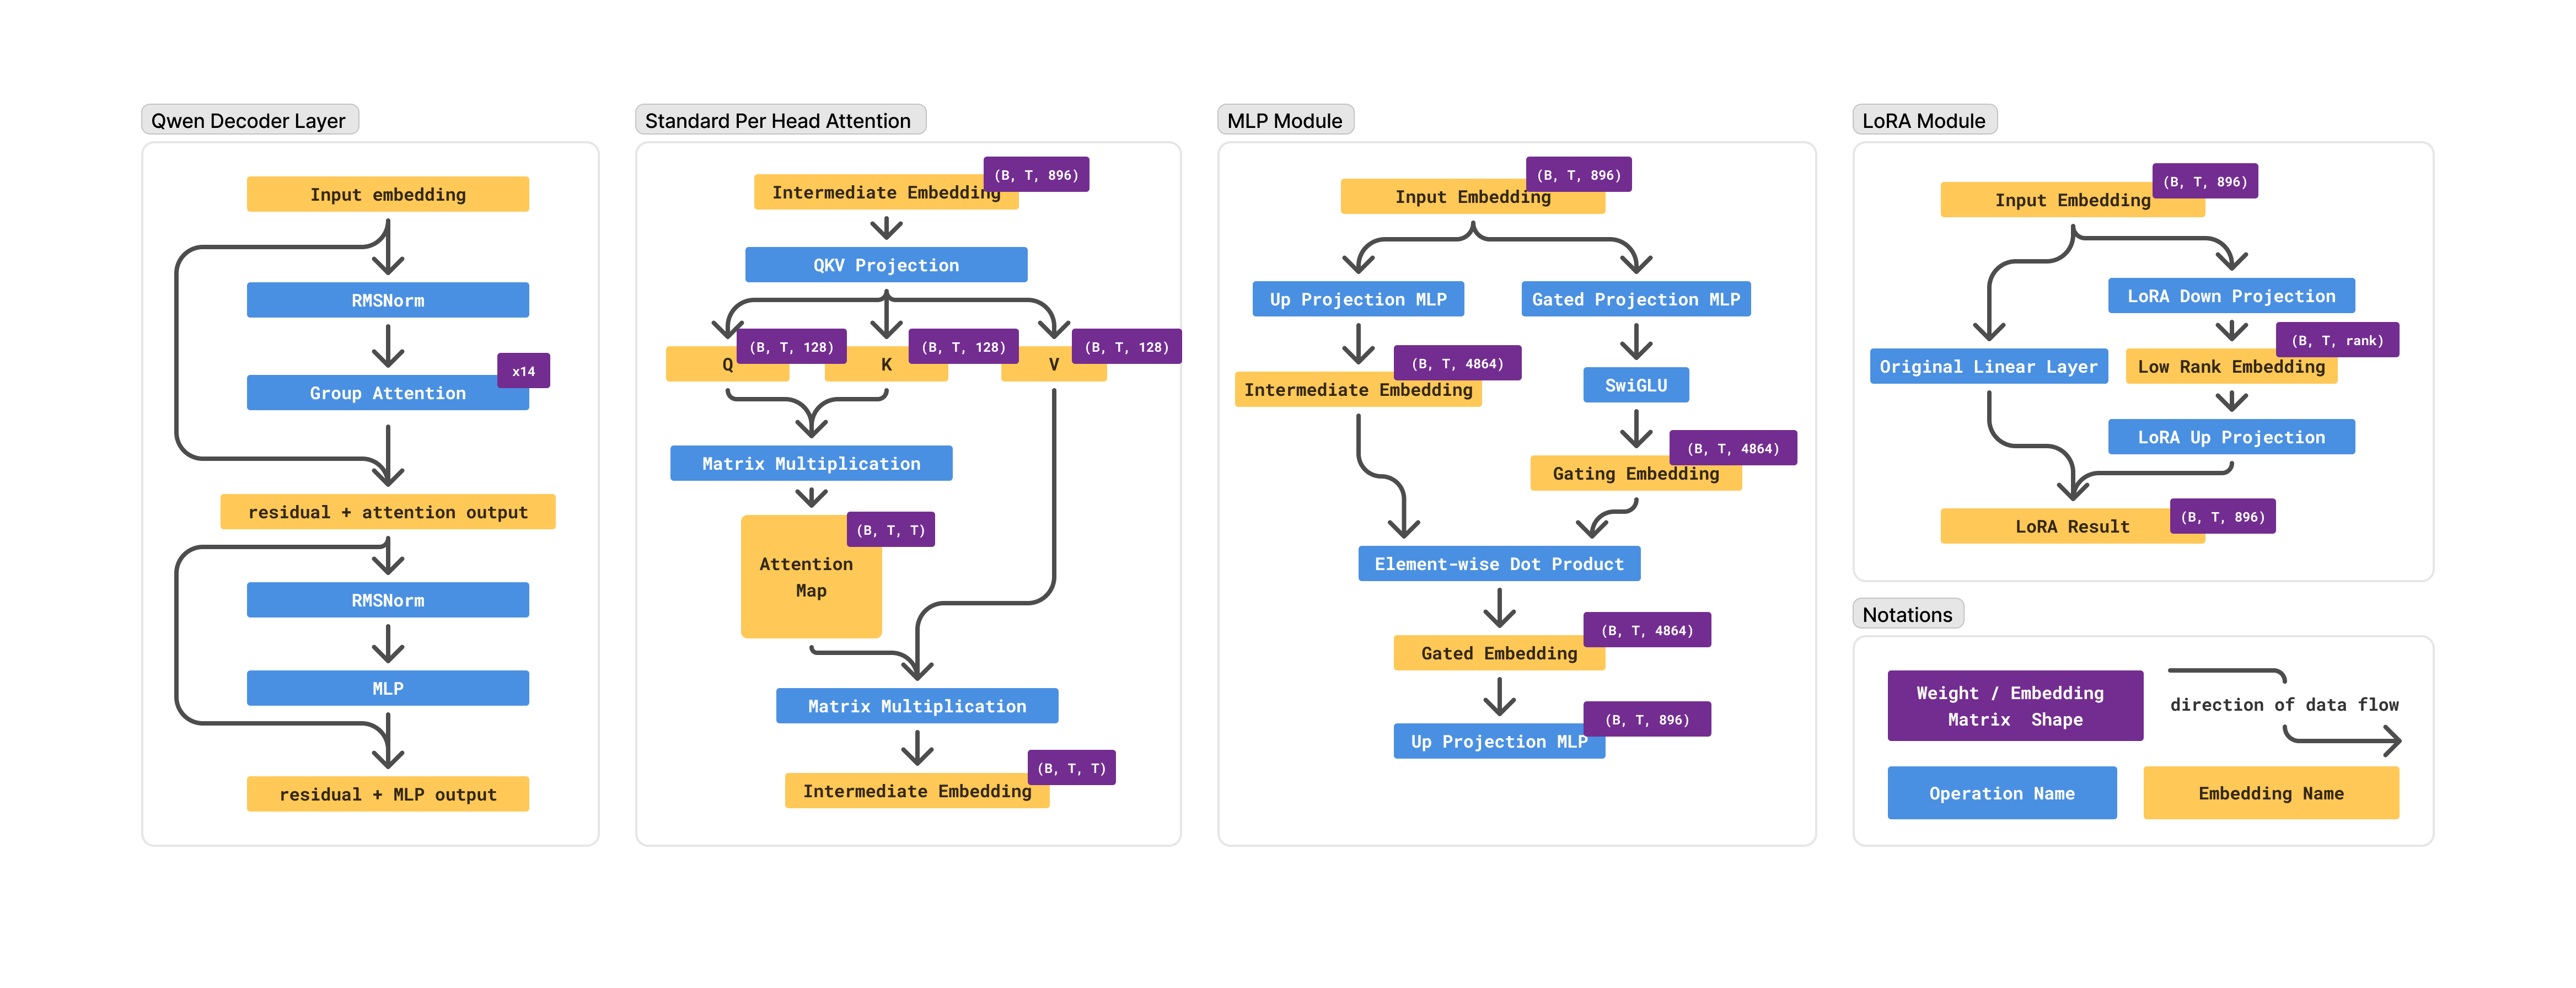
\includegraphics[width=\linewidth]{M2 Course Work/Images/Qwen_Arch.png}
    \caption{Architecture of Qwen 2.5 0.5B Model. The diagram details the overall model structure, including the Qwen Decoder Layer (stacked 24 times), single-head attention mechanism, MLP module, and LoRA (Low-Rank Adaptation) integration. Each component is annotated with data flow directions, embedding names, and tensor shapes to illustrate how input embeddings are transformed into predictions through normalization, multi-head attention, MLP gating, and low-rank updates.}
    \label{fig:Qwen_Arch}
\end{figure}

The \texttt{Qwen-2.5-0.5B-Instruct} model is composed of stacked decoder layers. Each layer primarily contains a Grouped Query Attention block and a Multilayer Perceptron block, both utilizing RMSNorm \cite{zhang2019rootmeansquarelayer} and residual connections \cite{he2015deepresiduallearningimage}. The MLP employs SwiGLU activation \cite{shazeer2020gluvariantsimprovetransformer}. For fine-tuning, LoRA \cite{hu2021loralowrankadaptationlarge} are applied to the query and key projection matrices within the attention mechanism. See Figure \ref{fig:Qwen_Arch}.

For FLOPS calculation, we followed the coursework guidelines and used Table \ref{tab:primitive_flops} for the flops costs on each primitive operations. The key hyper-parameters influencing FLOPS are batch size ($B$), sequence length ($S$), model dimensions (Table \ref{tab:notation}), and LoRA rank ($r$). The specific values used are listed in Table \ref{tab:notation}.

% Keep Notation Table
\begin{table}[!thbp]
\renewcommand{\arraystretch}{1.3} \centering \setlength{\tabcolsep}{8pt}
\begin{tabular}{@{}llc@{}} % Use @{} to remove padding
    \toprule
    \textbf{Symbol} & \textbf{Description} & \textbf{Value} \\ \midrule
    $B$           & Batch Size & 4 \\
    $S$           & Sequence Length & \textit{variable} (128, 512, 768) \\
    $H$           & Hidden/Model Dimension & 896 \\
    $H_{\text{mlp}}$ & MLP Intermediate Hidden Dimension & 4864 \\
    $N_{\text{heads}}$ & Number of Attention Heads & 14 \\
    $H_{\text{head}}$ & Dimension per Attention Head ($H / N_{\text{heads}}$) & 128 \tablefootnote{We assume the attention head dimension to be 128 (896 / 7), based on the original Qwen architecture, which uses a grouped query attention block with 2 groups and 14 heads. This results in 7 heads per group, with each group splitting the embedding dimension of 896 evenly, yielding a head dimension of 128.}\\
    $V_{\text{size}}$ & Vocabulary Size & 151936 \\
    $N_{\text{layers}}$ & Number of Qwen Decoder Layers & 24 \\
    $r$           & LoRA Rank & \textit{variable} (2, 4, 8) \\
    $\alpha$      & LoRA Scaling Factor & $r$ (common practice) \\ % Assumed alpha=r
    \bottomrule
\end{tabular}
\caption{Notation for FLOPS Calculation.}
\label{tab:notation}
\end{table}

% Keep Primitive FLOPS Table
\begin{table}[!thbp]
\renewcommand{\arraystretch}{1.4} \centering \setlength{\tabcolsep}{8pt}
\begin{tabular}{@{}lc@{}} % Use @{}
    \toprule
    \textbf{Operation} & \textbf{FLOPS} \\ \midrule
    Addition/Subtraction/Negation & 1 \\
    Multiplication/Division/Inverse & 1 \\
    ReLU/Absolute Value & 1 \\
    Exponentiation/Logarithm & 10 \\
    Sine/Cosine/Square Root & 10 \\
    \bottomrule
\end{tabular}
\caption{FLOPS Accounting for Primitives (per coursework Table 1).}
\label{tab:primitive_flops}
\end{table}

\subsection{FLOPs Estimation Approach}

We adopted a component-based approach, calculating the forward pass FLOPS for each distinct operation within a decoder layer: RMSNorm, Attention, MLP , LoRA, and Residual connections. The final LM head projection and loss computation were also included.

The detailed breakdown and formulas for each component are implemented in the script\footnote{\href{https://gitlab.developers.cam.ac.uk/phy/data-intensive-science-mphil/assessments/m2_coursework/ym429/-/blob/main/src/get_flops.py?ref_type=heads}{\texttt{src/get\_flops.py}}} and explained in the accompanying notebook\footnote{\href{https://gitlab.developers.cam.ac.uk/phy/data-intensive-science-mphil/assessments/m2_coursework/ym429/-/blob/main/notebooks/2_flops_calculation.ipynb?ref_type=heads}{\texttt{notebooks/2\_flops\_calculation.ipynb}}}.




\paragraph{Standard Multi-headed Attention ($Flops_{\text{Attention}}$)}
The attention module is the fundamental component of the Transformer architecture and modern LLMs. Given an input embedding $X \in \mathbb{R}^{B \times S \times H}$, it is first projected to Q, K, V embeddings using weight matrices $W_q, W_k, W_v \in \mathbb{R}^{H \times (N_{\text{heads}}H_{\text{head}})}$. 
\begin{equation}
    Q = X W_q, \quad K = X W_k, \quad V = X W_v 
\end{equation}
These matrices $Q, K, V \in \mathbb{R}^{B \times S \times (N_{\text{heads}}H_{\text{head}})}$ are then typically reshaped to $N_{\text{heads}}$ individual heads, yielding $Q_i, K_i, V_i \in \mathbb{R}^{B \times S \times H_{\text{head}}}$ for $i=1, ..., N_{\text{heads}}$. Rotary Positional Embeddings (RoPE) \cite{su2023roformerenhancedtransformerrotary} are applied to $Q_i$ and $K_i$. For the FLOPS of RoPE, we approximate it as simple element-wise addition operations.

The standard scaled dot-product attention is then computed per head:
\begin{equation}
    \text{Attention}(Q_i, K_i, V_i) = \text{Softmax}\left(\frac{Q_i K_i^T}{\sqrt{H_{\text{head}}}}\right) V_i, 
\end{equation}
where an causal mask is applied on $Q_i K_i^T$.
The outputs from all heads are then concatenated, $O = \text{Concat}(\text{Attention}_1, ..., \text{Attention}_{N_{\text{heads}}}) \in \mathbb{R}^{B \times S \times (N_{\text{heads}}H_{\text{head}})}$, and projected back to the hidden dimension using $W_o \in \mathbb{R}^{(N_{\text{heads}}H_{\text{head}}) \times H}$:
\begin{equation}
    X_{Attn} = O W_o
\end{equation}
FLOPS are detailed in Table \ref{tab:attention_flops}.

\begin{table}[!h]
\renewcommand{\arraystretch}{1.4} \centering \setlength{\tabcolsep}{8pt}
\begin{tabular}{@{}ll@{}} % Use @{}
    \toprule \textbf{Operation} & \textbf{Flops} \\ \midrule
    To Q, K, V & $Flops_{Mul} \cdot BSH \cdot 3 N_{h} H_{hd} + Flops_{Add} \cdot BS(H-1) \cdot 3 N_{h} H_{hd}$ \\ % Simplified notation
    Add ROPE & $Flops_{Add} \cdot BS \cdot 2 N_{h} H_{hd}$ \\ % Adjusted based on typical RoPE application to Q, K
    $QK^T$ & $Flops_{Mul} \cdot B N_{h} S H_{hd} S + Flops_{Add} \cdot B N_{h} S (H_{hd}-1) S$ \\
    Scale by $1/\sqrt{H_{head}}$ & $Flops_{SQRT} + Flops_{DIV} \cdot B N_{h} S S$ \\ % Simplified scaling cost
    Add Mask & $Flops_{Add} \cdot B N_{h} S S$ \\ % Simplified mask cost
    Softmax & $(Flops_{EXP} + Flops_{Add} \times (S-1) + Flops_{DIV}) \cdot B N_{h} S S$ \\ % Simplified Softmax cost
    Multiply by V & $Flops_{MUL} \cdot B N_{h} S S H_{hd} + Flops_{ADD} \cdot B N_{h} S (S - 1) H_{hd}$ \\
    Output Projection ($W_o$) & $Flops_{MUL} \cdot B S (N_{h} H_{hd}) H + Flops_{ADD} \cdot B S (N_{h} H_{hd} - 1) H$ \\
    \bottomrule
\end{tabular}
\caption{FLOPS Breakdown for Attention Mechanism Layer (Standard MHA). $N_h$ = $N_{\text{heads}}$, $H_{hd}$ = $H_{\text{head}}$.} % Added notation clarification
\label{tab:attention_flops}
\end{table}

\paragraph{RMSNorm ($Flops_{\text{RMSNorm}}$)}
normalizes input $x \in \mathbb{R}^{B \times S \times H}$ across the hidden dimension $H$ with the root mean square of the embedding, scaled by a learnable parameter $\gamma$. Mathematically, it can be represented as:
\begin{equation}
    \text{RMS}(x) = \sqrt{\frac{1}{H} \sum_{i=1}^{H} x_i^2 + \epsilon}
\end{equation}
\begin{equation}
    y_i = \frac{x_i}{\text{RMS}(x)} \gamma_i
\end{equation}

% Keep RMSNorm FLOPS Table (Minor text edits in caption possible for brevity if needed)
\begin{table}[!thbp]
\renewcommand{\arraystretch}{1.4} \centering \setlength{\tabcolsep}{8pt}
\begin{tabular}{@{}ll@{}} % Use @{}
    \toprule \textbf{Operation} & \textbf{Flops} \\ \midrule
    Square elements & $Flops_{Mul} \cdot BSH$ \\
    Mean over H & $Flops_{Add} \cdot BS(H - 1) + Flops_{Div} \cdot BS$ \\
    Add epsilon & $Flops_{Add} \cdot BS$ \\
    Square root & $Flops_{Sqrt} \cdot BS$ \\
    Reciprocal (rsqrt) & $Flops_{Div} \cdot BS$ \\
    Normalize input & $Flops_{Mul} \cdot BSH$ \\
    Scale by $\gamma$ & $Flops_{Mul} \cdot BSH$ \\
    \bottomrule
\end{tabular}
\caption{FLOPS Breakdown for RMSNorm Layer.} \label{tab:rmsnorm_flops}
\end{table}

\paragraph{MLP ($Flops_{\text{MLP}}$)}
Qwen's MLP module use a SwiGLU activation with two linear layers \cite{shazeer2020gluvariantsimprovetransformer}. For an input $x \in \mathbb{R}^{B \times S \times H}$, it's first projected to an intermediate dimension $H_{\text{mlp}}$ using two weights $W_{up}, W_{gate}\in \mathbb{R}^{H \times H_{MLP}}$. The gated projection is activated with SiLU:
$$
\text{SiLU}(z)=z\cdot\text{sigmoid}(z),
$$
and element-wise multiplied with the up projected embedding. These operation can be seen as the SwiGLU activation. A down-projection with $W_{down}\in \mathbb{R}^{ H_{MLP}\times H}$ restores the embedding to the hidden dimension:
\begin{equation}
    X_{MLP} = \left[ (X W_{up}) \odot \text{SiLU}(X W_{gate}) \right] W_{down}
\end{equation}

FLOPS are in Table \ref{tab:ffn_glu_flops}.

% Keep MLP FLOPS Table (Minor text edits in caption possible for brevity if needed)
\begin{table}[!thbp]
\renewcommand{\arraystretch}{1.4} \centering \setlength{\tabcolsep}{8pt}
\begin{tabular}{@{}ll@{}} % Use @{}
    \toprule \textbf{Operation} & \textbf{Flops} \\ \midrule
    Gate Projection ($W_{gate}$) & $Flops_{Mul} \cdot BSH H_{mlp} + Flops_{Add} \cdot BS(H - 1) H_{mlp}$ \\
    SiLU Activation & $(Flops_{Neg} + Flops_{Exp} + Flops_{Add} + Flops_{Div} + Flops_{Mul}) \cdot BS H_{mlp}$ \\
    Up Projection ($W_{up}$) & $Flops_{Mul} \cdot BSH H_{mlp} + Flops_{Add} \cdot BS(H - 1) H_{mlp}$ \\
    Element-wise Mult & $Flops_{Mul} \cdot BS H_{mlp}$ \\
    Down Projection ($W_{down}$) & $Flops_{Mul} \cdot BS H_{mlp} H + Flops_{Add} \cdot BS(H_{mlp} - 1) H$ \\
    \bottomrule
\end{tabular}
\caption{FLOPS Breakdown for MLP Layer with SwiGLU.} \label{tab:ffn_glu_flops}
\end{table}

\paragraph{LoRA \cite{hu2021loralowrankadaptationlarge} ($Flops_{\text{LoRA}}$)} is a parameter-efficient fine-tuning technique that freezes the full LLM model while injecting two low-rank, trainable weight matrices into each q and k projection of the multi-headed attention layers. These matrices effectively mimic the weight updates from full fine-tuning, allowing efficient adaptation by tuning only a fraction of the parameters. For an input $x$, the output of a LoRA-adapted linear layer is given by:
\begin{equation}
    y = xW + x A B (\alpha / r),
\end{equation}
where $A \in \mathbb{R}^{d_{in} \times r}$ and $B \in \mathbb{R}^{r \times d_{out}}$ are the trainable low-rank matrices, $r$ denotes the rank, $\alpha$ is a scaling factor, $d_{in}$ is the input dimension, and $d_{out}$ is the output dimension. Table \ref{tab:lora_flops} details the FLOPS for the LoRA path ($x A B (\alpha / r)$), representing the additional computational cost to the Q/K projection layer. For Q/K projections, we have $d_{in}=H$ and $d_{out}=H_{head}N_{heads}$.

\begin{table}[!thbp]
\renewcommand{\arraystretch}{1.4} \centering \setlength{\tabcolsep}{8pt}
\begin{tabular}{@{}ll@{}} % Use @{}
    \toprule \textbf{Operation} & \textbf{Flops} \\ \midrule
    Down Projection (A) & $Flops_{Mul} \cdot BSH r + Flops_{Add} \cdot BS(H - 1) r$ \\ % Use 'r' for rank
    Up Projection (B) & $Flops_{Mul} \cdot BS r (N_{h} H_{hd}) + Flops_{Add} \cdot BS(r - 1) (N_{h} H_{hd})$ \\ % Use N_h, H_hd
    Scaling ($\alpha/r$) & $Flops_{Mul} \cdot BS (N_{h} H_{hd})$ \\
    Addition to Original & $Flops_{Add} \cdot BS (N_{h} H_{hd})$ \\
    \bottomrule
\end{tabular}
\caption{FLOPS Breakdown for LoRA} \label{tab:lora_flops}
\end{table}

\paragraph{Residual Connection ($Flops_{\text{Residual}}$)}
Adds the input of a block to its output: 
$$X_{out} = X_{in} + \text{Block}(X_{in}).$$ FLOPS are in Table \ref{tab:residual_flops}.

% Keep Residual FLOPS Table (Minor text edits in caption possible for brevity if needed)
\begin{table}[!thbp]
\renewcommand{\arraystretch}{1.4} \centering \setlength{\tabcolsep}{8pt}
\begin{tabular}{@{}ll@{}} % Use @{}
    \toprule \textbf{Operation} & \textbf{Flops} \\ \midrule
    Element-wise Addition & $Flops_{Add} \cdot BSH$ \\
    \bottomrule
\end{tabular}
\caption{FLOPS Breakdown for Residual Connection.} \label{tab:residual_flops}
\end{table}

\paragraph{LM Head and Loss ($Flops_{\text{LM Head + Loss}}$)} represents the last layer of Qwen model, which
projects the final decoder layer's output $X_{final} \in \mathbb{R}^{B \times S \times H}$ to vocabulary size $V_{\text{size}}$, applies Softmax, and computes Cross-Entropy loss. FLOPS are in Table \ref{tab:lm_head_flops}.

\begin{table}[!thbp]
\renewcommand{\arraystretch}{1.4} \centering \setlength{\tabcolsep}{8pt}
\begin{tabular}{@{}ll@{}} % Use @{}
    \toprule \textbf{Operation} & \textbf{Flops} \\ \midrule
    LM Head Projection & $Flops_{Mul} \cdot BSH V_{size} + Flops_{Add} \cdot BS(H - 1) V_{size}$ \\
    LM Head Bias & $Flops_{Add} \cdot BS V_{size}$ \\ % Assuming bias exists
    Softmax & $(Flops_{Exp} + Flops_{Add} \times (V_{size}-1) + Flops_{Div}) \cdot BS V_{size}$ \\ % Simplified Softmax cost
    Log Loss (per token) & $(Flops_{Log} + Flops_{Mul}) \cdot BS$ \\ % Simplified Loss cost
    \bottomrule
\end{tabular}
\caption{FLOPS Breakdown for LM Head and Final Operations.} \label{tab:lm_head_flops}
\end{table}

\subsection{Total FLOPS Estimation}

To conclude, the FLOPS for one forward pass through a single Qwen decoder layer is:
\begin{align}
Flops_{\text{Layer}} &= Flops_{\text{RMSNorm}} + (Flops_{\text{Attention}} + 2 \times Flops_{\text{LoRA}}) \nonumber \\
                     &+ Flops_{\text{Residual}} + Flops_{\text{RMSNorm}} + Flops_{\text{MLP}} \nonumber \\
                     &+ Flops_{\text{Residual}} \label{eq:qwen_layer_flops}
\end{align}
Total inference FLOPS for the model is then:
\begin{equation}
Flops_{\text{Inference}} = N_{\text{layers}} \times Flops_{\text{Layer}} + Flops_{\text{LM Head + Loss}}
\label{eq:qwen_inference_flops_revised}
\end{equation}
Total training step FLOPS (forward + backward):
\begin{equation}
Flops_{\text{Training Step}} \approx 3 \times Flops_{\text{Inference}}
\label{eq:qwen_training_flops_revised}
\end{equation}
This estimate (Equation \ref{eq:qwen_training_flops_revised}) guided our experimental planning.

\subsection{Experiment Planning within FLOPS Budget}

Equation \ref{eq:qwen_training_flops_revised} allowed calculation of FLOPS per step for various configurations (Table \ref{tab:flops_vs_steps}).

% Keep FLOPS vs Steps Table (No changes needed)
\begin{table}[!htbp]
\renewcommand{\arraystretch}{1.4} \centering \setlength{\tabcolsep}{8pt}
\begin{tabular}{@{}ccrr@{}}
    \toprule \textbf{Context Length ($S$)} & \textbf{Rank ($r$)} & \textbf{FLOPS per Step} & \textbf{Max Steps (Budget)} \\ \midrule
    128 & 2 &  1.90 $\times 10^{12}$ & 52,743 \\
    128 & 4 &  1.90 $\times 10^{12}$ & 52,738 \\
    128 & 8 &  1.90 $\times 10^{12}$ & 52,728 \\ \midrule
    512 & 2 &  8.00 $\times 10^{12}$ & 12,500 \\
    512 & 4 &  8.00 $\times 10^{12}$ & 12,499 \\
    512 & 8 &  8.00 $\times 10^{12}$ & 12,496 \\ \midrule
    768 & 2 & 1.24 $\times 10^{13}$ & 8,054 \\
    768 & 4 & 1.24 $\times 10^{13}$ & 8,053 \\
    768 & 8 & 1.24 $\times 10^{13}$ & 8,052 \\
    \bottomrule
\end{tabular}
\caption{Calculated FLOPS per training step (Batch Size $B=4$) and theoretical maximum optimizer steps within the $1 \times 10^{17}$ FLOPS budget.} \label{tab:flops_vs_steps}
\end{table}

Overall, the total budget allows us to run around 10,000 runs for $B=4$, and needs to accommodate initial tests, grid searches (12 runs), and final training. Therefore, we allocated steps per phase (Table \ref{tab:training_steps}), using short runs for exploration and reserving budget for the final model. This FLOPS-aware planning before training was essential to the success of the final resulting model.

% Keep Training Steps Table (No changes needed)
\begin{table}[!htbp]
\renewcommand{\arraystretch}{1.4} \centering \setlength{\tabcolsep}{8pt}
\begin{tabular}{@{}lr@{}}
    \toprule \textbf{Training Phase} & \textbf{Planned Optimizer Steps} \\ \midrule
    Initial Training / Smoke Test & 1,000 \\
    Grid Search Runs (per run)\textsuperscript{a} & 500 \textsuperscript{b} \\
    Final Model Training & $\approx$ 3,000\textsuperscript{c} \\
    \bottomrule
\end{tabular}
\caption{Planned optimizer step allocation per training phase. \newline
\textsuperscript{a}Applies to each grid search experiment (learning rate, rank) and search over context length. \newline
\textsuperscript{b}The design of 500 steps allows the model to see the entire dataset at least 1 time ($\approx 1.2$ epoch). \newline
\textsuperscript{c}Flexible, utilizing remaining budget after searches (estimated 2k-4k steps).} \label{tab:training_steps}
\end{table}



\section{Experimental Setup}
\label{sec:setup}

Our experimental process followed four main phases, designed for systematic exploration within the FLOPS budget: 1) Initial baseline training, 2) Grid search over LoRA rank ($r$) and learning rate ($\eta$), 3) Search over context length ($S$), and 4) Final training with the optimized configuration.

\paragraph{Data Handling}
\label{sec:data-handling}
The Lotka-Volterra dataset (Section \ref{sec:dataset}) was split into training (80\%), validation (10\%), and test (10\%) sets. Each time series was processed using the LLMTime method (Section \ref{sec:preprocessing}) into a token sequence. Due to model input limits, these sequences ($\approx$ 1000 tokens/system) were chunked into smaller segments of context length $S \in \{128, 512, 768\}$. We used a sliding window with a stride of 256 tokens to generate overlapping chunks, maximizing data use.

A critical issue encountered was input padding. The \texttt{Qwen} model requires left-padding, conflicting with the \href{https://gitlab.developers.cam.ac.uk/phy/data-intensive-science-mphil/lecture-materials/m2_dl_for_dis/-/blob/main/coursework/lora_skeleton.py?ref_type=heads}{right-padding provided in the \texttt{lora\_skeleton} code}. Right-padding disrupted model behaviour (affecting the causal attention mask and positional encoding interpretation), leading to non-numerical outputs (Figure \ref{fig:padding_effect}). As this was only discovered after the full training, a workaround was implemented: only full-length sequence chunks (exactly matching $S$ and requiring no padding) were used for training and evaluation. Shorter chunks, mainly from the end of time series, were discarded. This ensured correct model operation without padding but potentially excluded some data, a limitation discussed in Section \ref{sec:discussion}.

% Keep padding figure
\begin{figure}[!htbp]
    \centering
    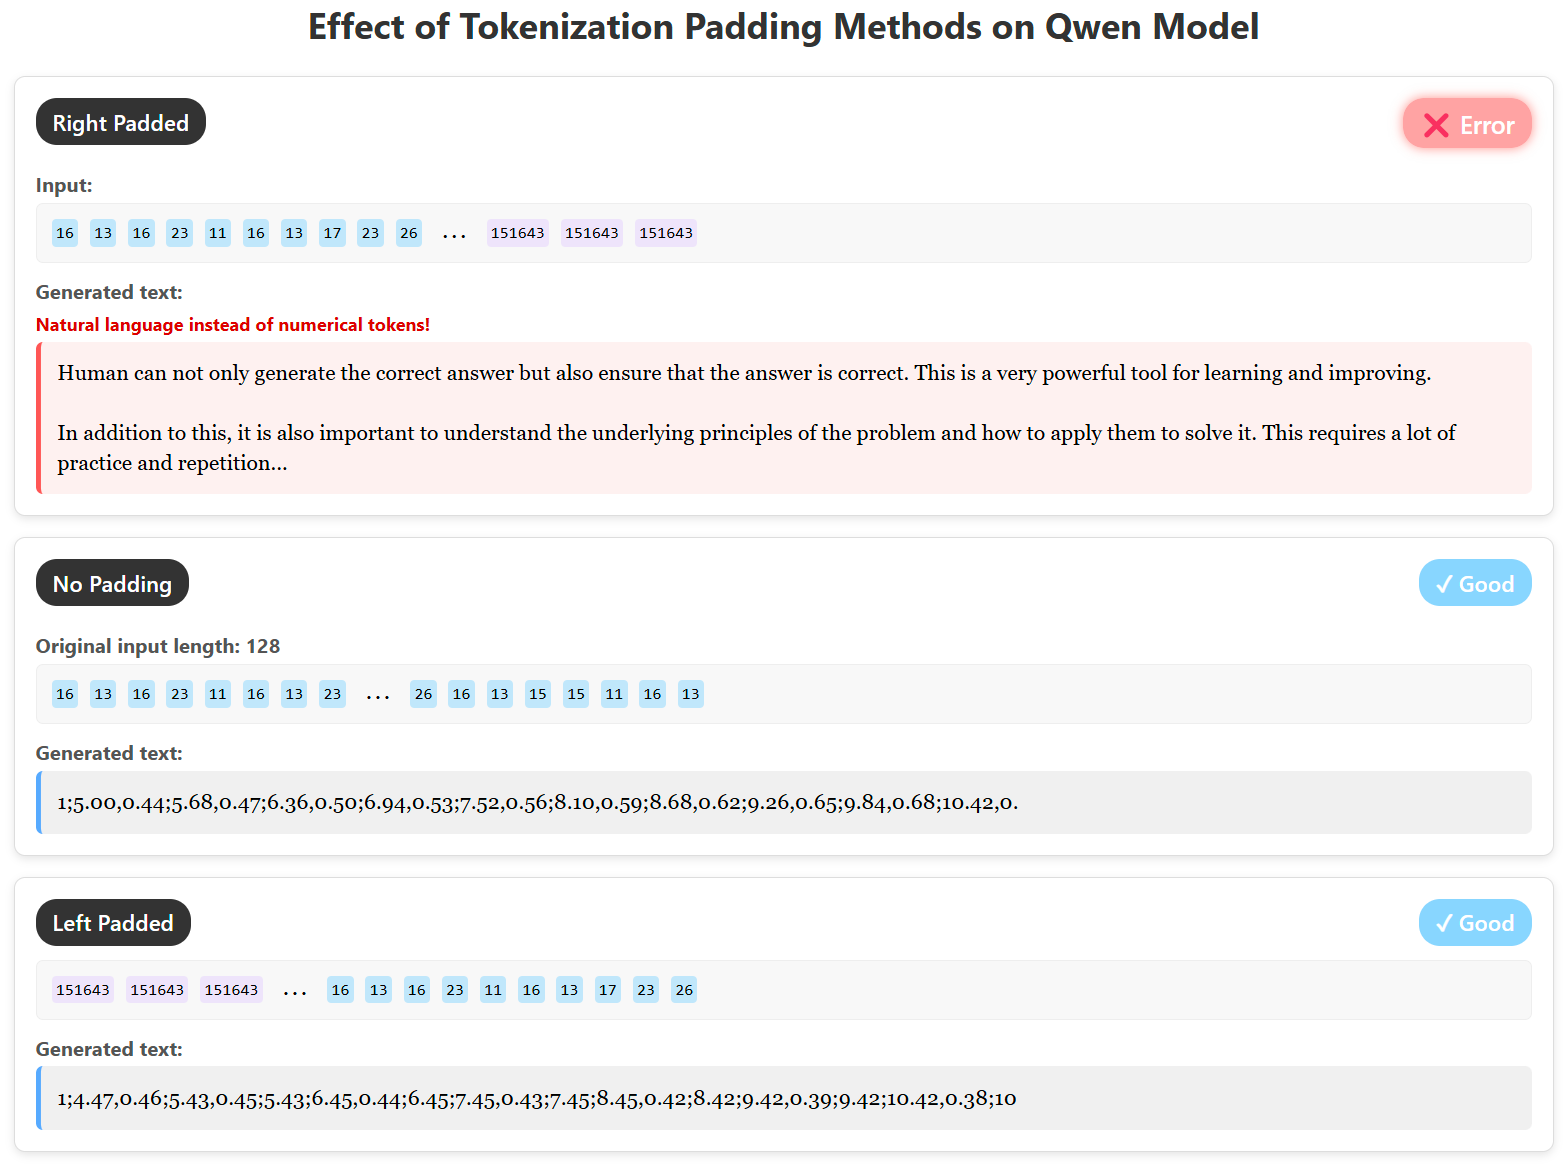
\includegraphics[width=0.9\linewidth]{M2 Course Work//Images/padding_effect.png}
    \caption{Effect of padding on \texttt{Qwen} output. Right-padding (Top) causes failure. Using only full sequences (Middle) or correct left-padding (Bottom) yields expected numerical format.} % Shortened caption
    \label{fig:padding_effect}
\end{figure}


\paragraph{Training and Evaluation}
All models were trained using the AdamW optimizer \cite{loshchilov2019decoupledweightdecayregularization}. During training, performance was evaluated on the validation set every 50 optimizer steps recording the validation loss. The model checkpoint with the lowest validation loss was saved and used for final evaluation. At all cases, the validation set was used exclusively for model selection, while only the untrained \ref{sec:untrained}, initial \ref{sec:initial}, and final \ref{sec:final} models were evaluated on the test set, which was never used for parameter tuning.


Final performance was measured using Mean Squared Error (MSE) and Mean Absolute Error (MAE) between the model's predicted numerical sequences and the ground truth sequences. \textbf{Note that the MSE and MAE are calculated on decoded time-series data, not on the tokens.} Notably, the MSE and MAE show little difference at the first prediction step. However, as prediction errors accumulate over time in autoregressive models, evaluating performance over multiple steps provides a more sensitive measure of the model’s capability. That said, if too many prediction steps are considered, even well-performing models can degrade significantly due to accumulated errors, making them appear indistinguishable from poorer models. To strike a balance, we conducted an initial analysis (Figure \ref{fig:metric-diff-between-timestamp}) to determine a sensible number of future steps for evaluation. Based on this, we found that using five prediction steps ($\approx 50 - 60$ tokens)—averaging the MSE and MAE across them—offers a meaningful and stable metric for comparing model performance.


% Keep metric diff figure (assuming it shows error divergence over steps)
\begin{figure}[!htbp] % Changed from figure to figure[!htbp]
    \centering
    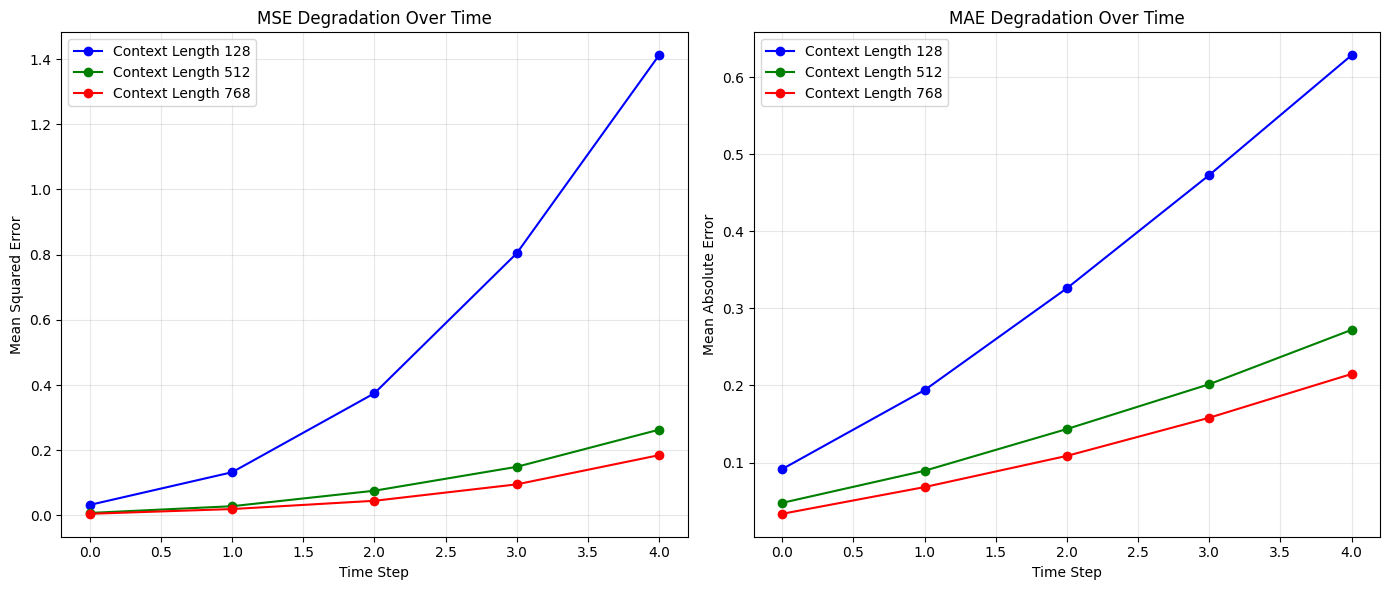
\includegraphics[width=0.9\linewidth]{M2 Course Work//Images/metric_diff_between_timestamp.png} % Adjusted width
    \caption{Example of increasing prediction error (e.g., MAE) over successive prediction time steps for different configurations. Note that at the fifth time-stamp, there is already a significant enough gap between the result of different context-length evaluation, thus motivating the 5-step average evaluation approach.} % Improved caption
    \label{fig:metric-diff-between-timestamp}
\end{figure}


\begin{figure}[!htbp]
    \centering
    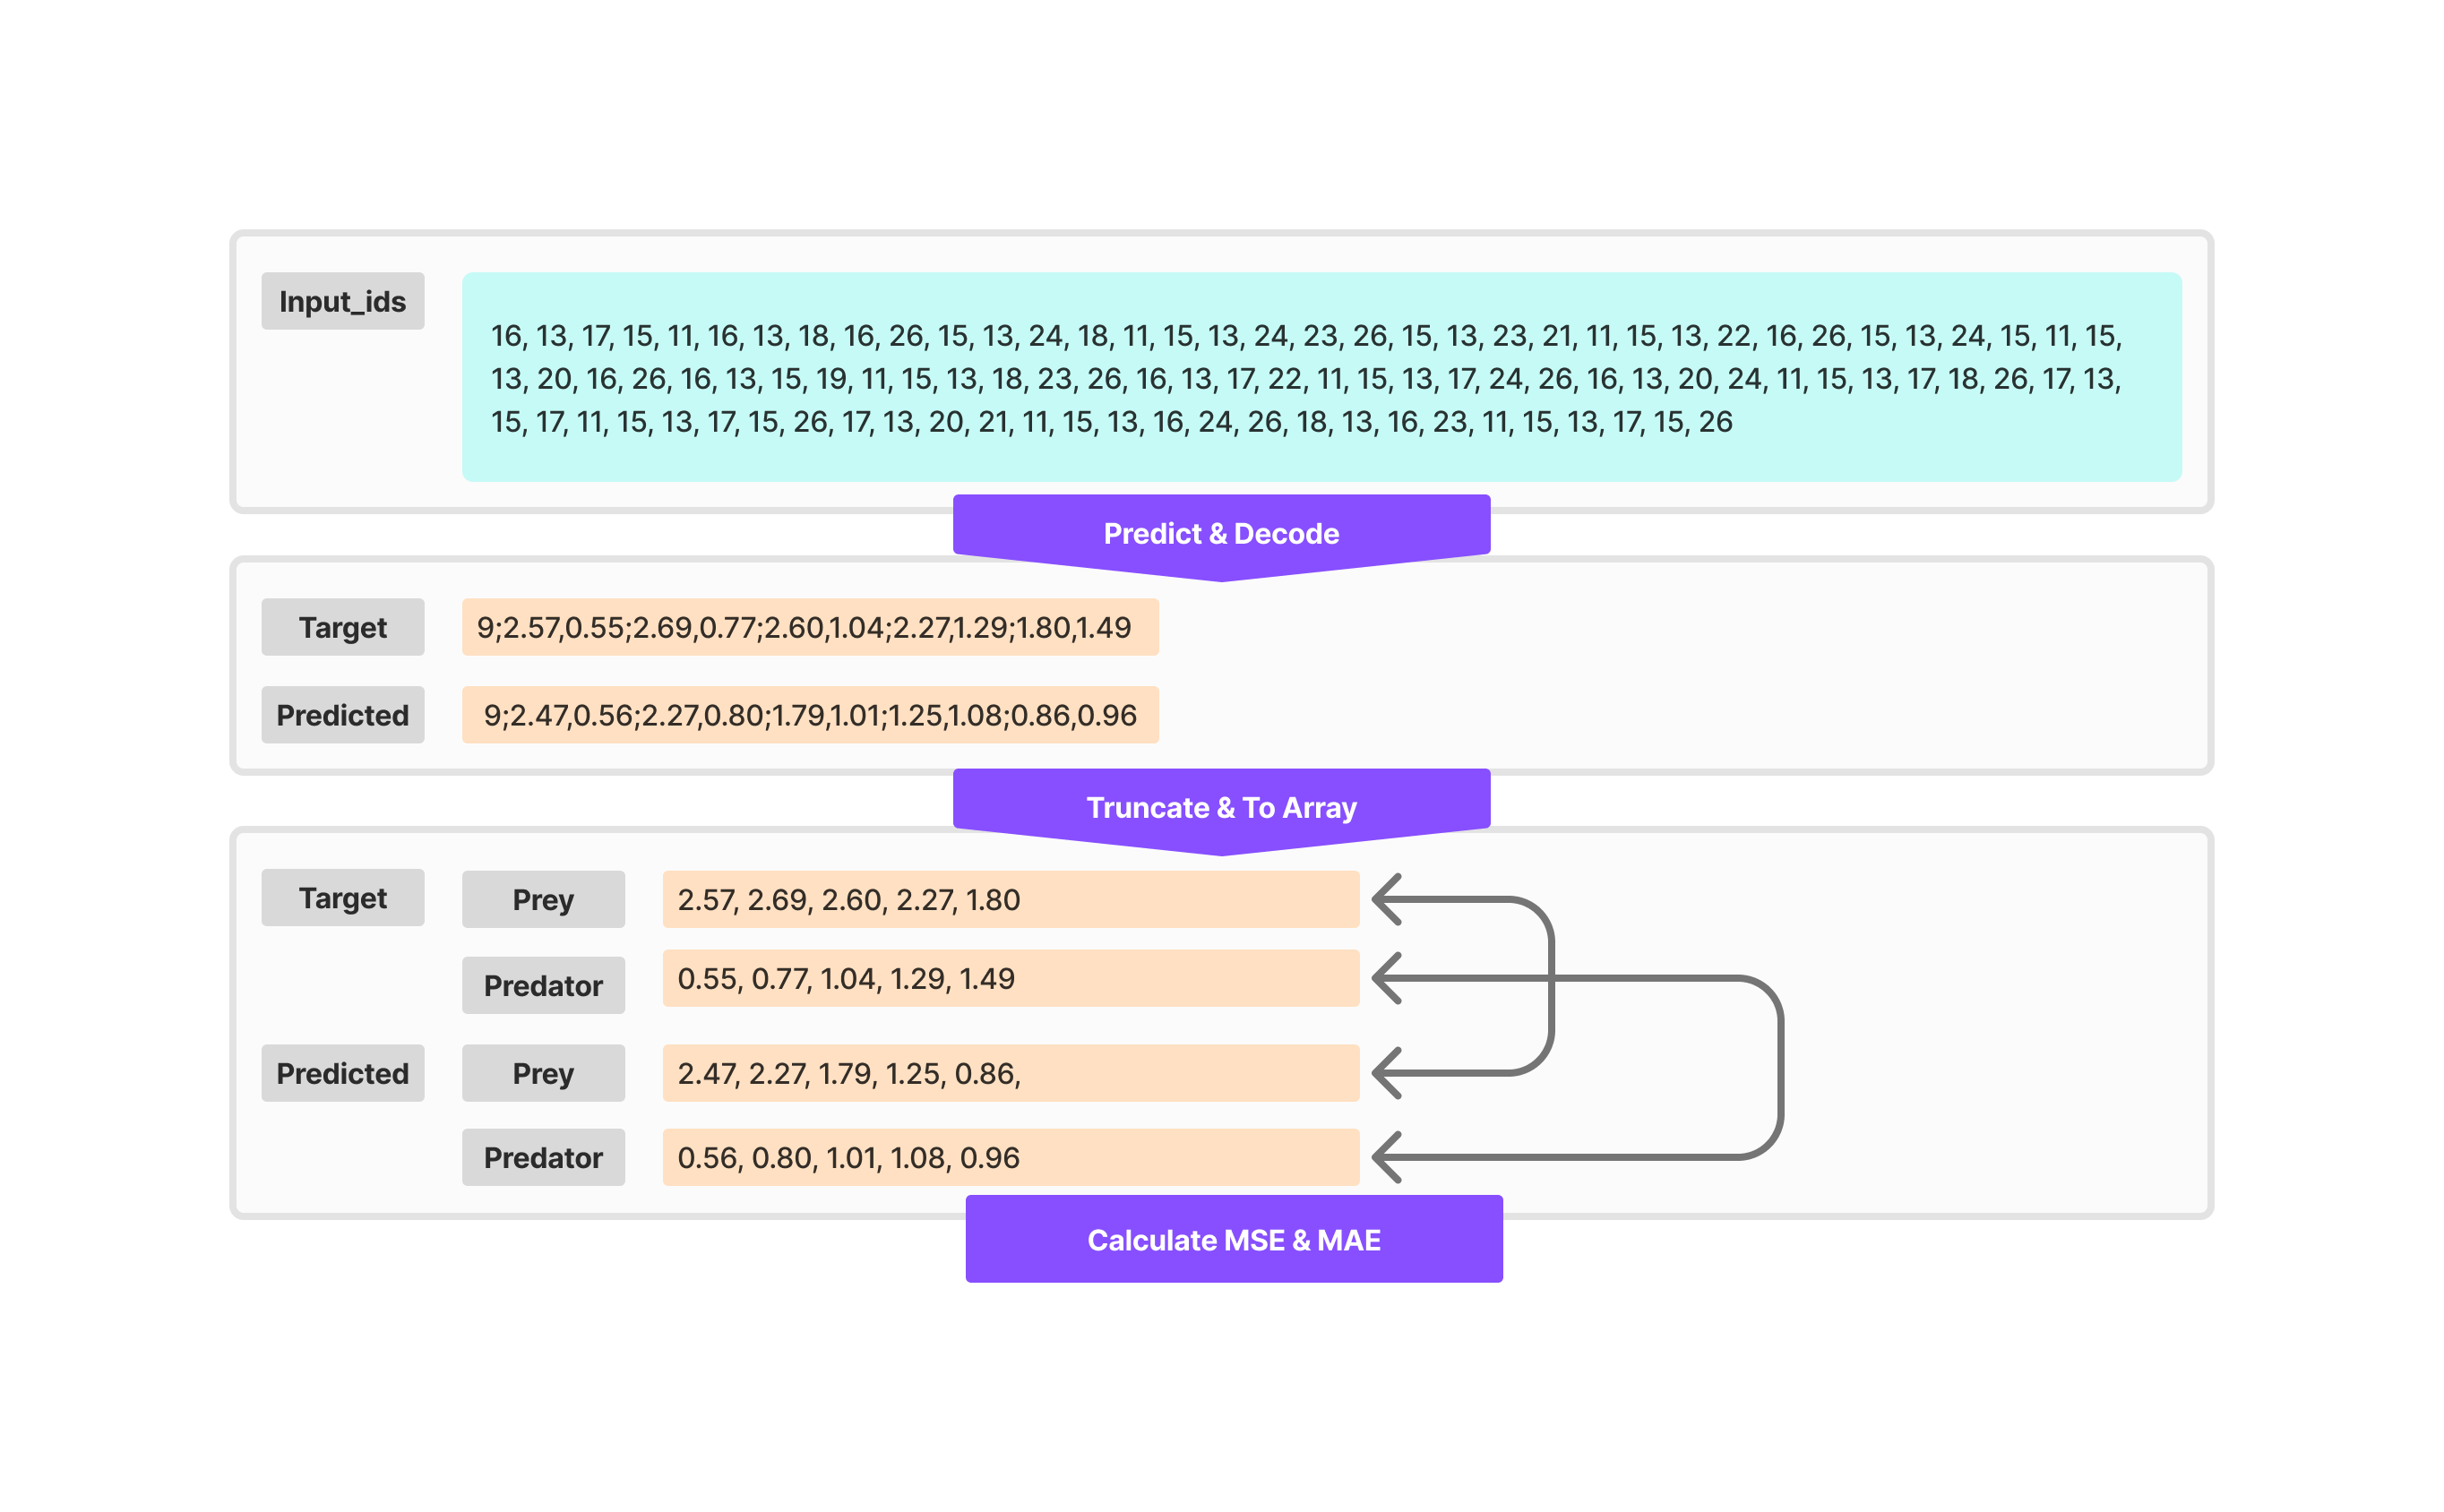
\includegraphics[width=0.8\linewidth]{M2 Course Work//Images/Metric_calculation.png}
    \caption{Model Evaluation Process: Given the model's decoded predictions and target data, only the first five complete time steps are retained by truncating from the first to the sixth semicolon. The resulting text is then converted into numerical arrays and compared against the target values. Finally, Mean Squared Error (MSE) and Mean Absolute Error (MAE) are computed to assess prediction accuracy.}
    \label{fig:metric-calculation}
\end{figure}


\section{Results}
\label{sec:results}

This section presents the performance evaluation of the \texttt{Qwen} model at different stages. Performance is primarily assessed using Mean Squared Error (MSE) and Mean Absolute Error (MAE) on the test set, averaged over a 5-step prediction as described in Section \ref{sec:setup}. Table \ref{tab:training_stage_comparison} summarizes the key metrics across stages.

\subsection{Untrained Baseline Performance (Q2b)}
\label{sec:untrained}
Initially, the pre-trained \texttt{Qwen} model was evaluated without any fine-tuning (zero-shot) to establish a baseline. As shown in Table \ref{tab:training_stage_comparison} (Untrained), the performance was poor, with high MSE and MAE values. This is expected, given the model's pre-training on natural language. A noticeable trend was better performance (lower errors) with longer context lengths ($S$), suggesting some inherent ability to leverage longer history, even if poorly. Visualizations (Figure \ref{fig:untrained_predictions} in Appendix) confirm the lack of task understanding, with predictions often being constant or near-constant values, failing entirely to capture the cyclical dynamics of the Lotka-Volterra systems.

% Keep Table: Training Stage Comparison
\begin{table}[!htbp] % Use htbp for better placement
\renewcommand{\arraystretch}{1.4} \centering \setlength{\tabcolsep}{8pt}
% \sisetup{round-mode=places, round-precision=6} % Optional siunitx setup
\begin{tabular}{@{}c rr rr rr@{}} % Use @{}
    \toprule
    & \multicolumn{2}{c}{\textbf{Untrained}}
    & \multicolumn{2}{c}{\textbf{Initial Training}}
    & \multicolumn{2}{c}{\textbf{Final Training}} \\
    \cmidrule(lr){2-3} \cmidrule(lr){4-5} \cmidrule(lr){6-7}
    \textbf{Context ($S$)} & \textbf{MSE} & \textbf{MAE} & \textbf{MSE} & \textbf{MAE} & \textbf{MSE} & \textbf{MAE} \\ \midrule
    128 & 0.5510 & 0.3427 & 0.1356 & 0.1746 & 0.0263 & 0.0726 \\ % Rounded for brevity
    512 & 0.1048 & 0.1509 & 0.0362 & 0.0834 & 0.0028 & 0.0240 \\
    768 & 0.0700 & 0.1167 & 0.0297 & 0.0651 & 0.0020 & 0.0191 \\
    \bottomrule
\end{tabular}
\caption{Test set performance (averaged over 5 prediction steps) across training stages. Initial training: 1000 steps ($S=512, \eta=10^{-4}, r=4$). Final training: Optimized ($\eta=10^{-4}, r=8, S=768$).} % Shortened caption
\label{tab:training_stage_comparison}
\end{table}


\subsection{Initial LoRA Training (Q3a)}
\label{sec:initial}

The model was then fine-tuned for 1000 steps using default hyper-parameters ($S=512, \eta=10^{-4}, r=4$). LoRA is applied to all q and k layers of attention module. Therefore, the parameters that are been tuned are all the \texttt{model.model.layers[i].self\_attn.q\_proj.A} and \texttt{model.model.layers[i]. self\_attn.q\_proj.B}, for $i \in \{0, \cdots, 23\}$ and \texttt{model.model.lm\_head.bias}.

% Keep Figure: Initial Loss Curves
\begin{figure}[!h]
    \centering
    \begin{subfigure}[b]{0.48\linewidth} \centering
        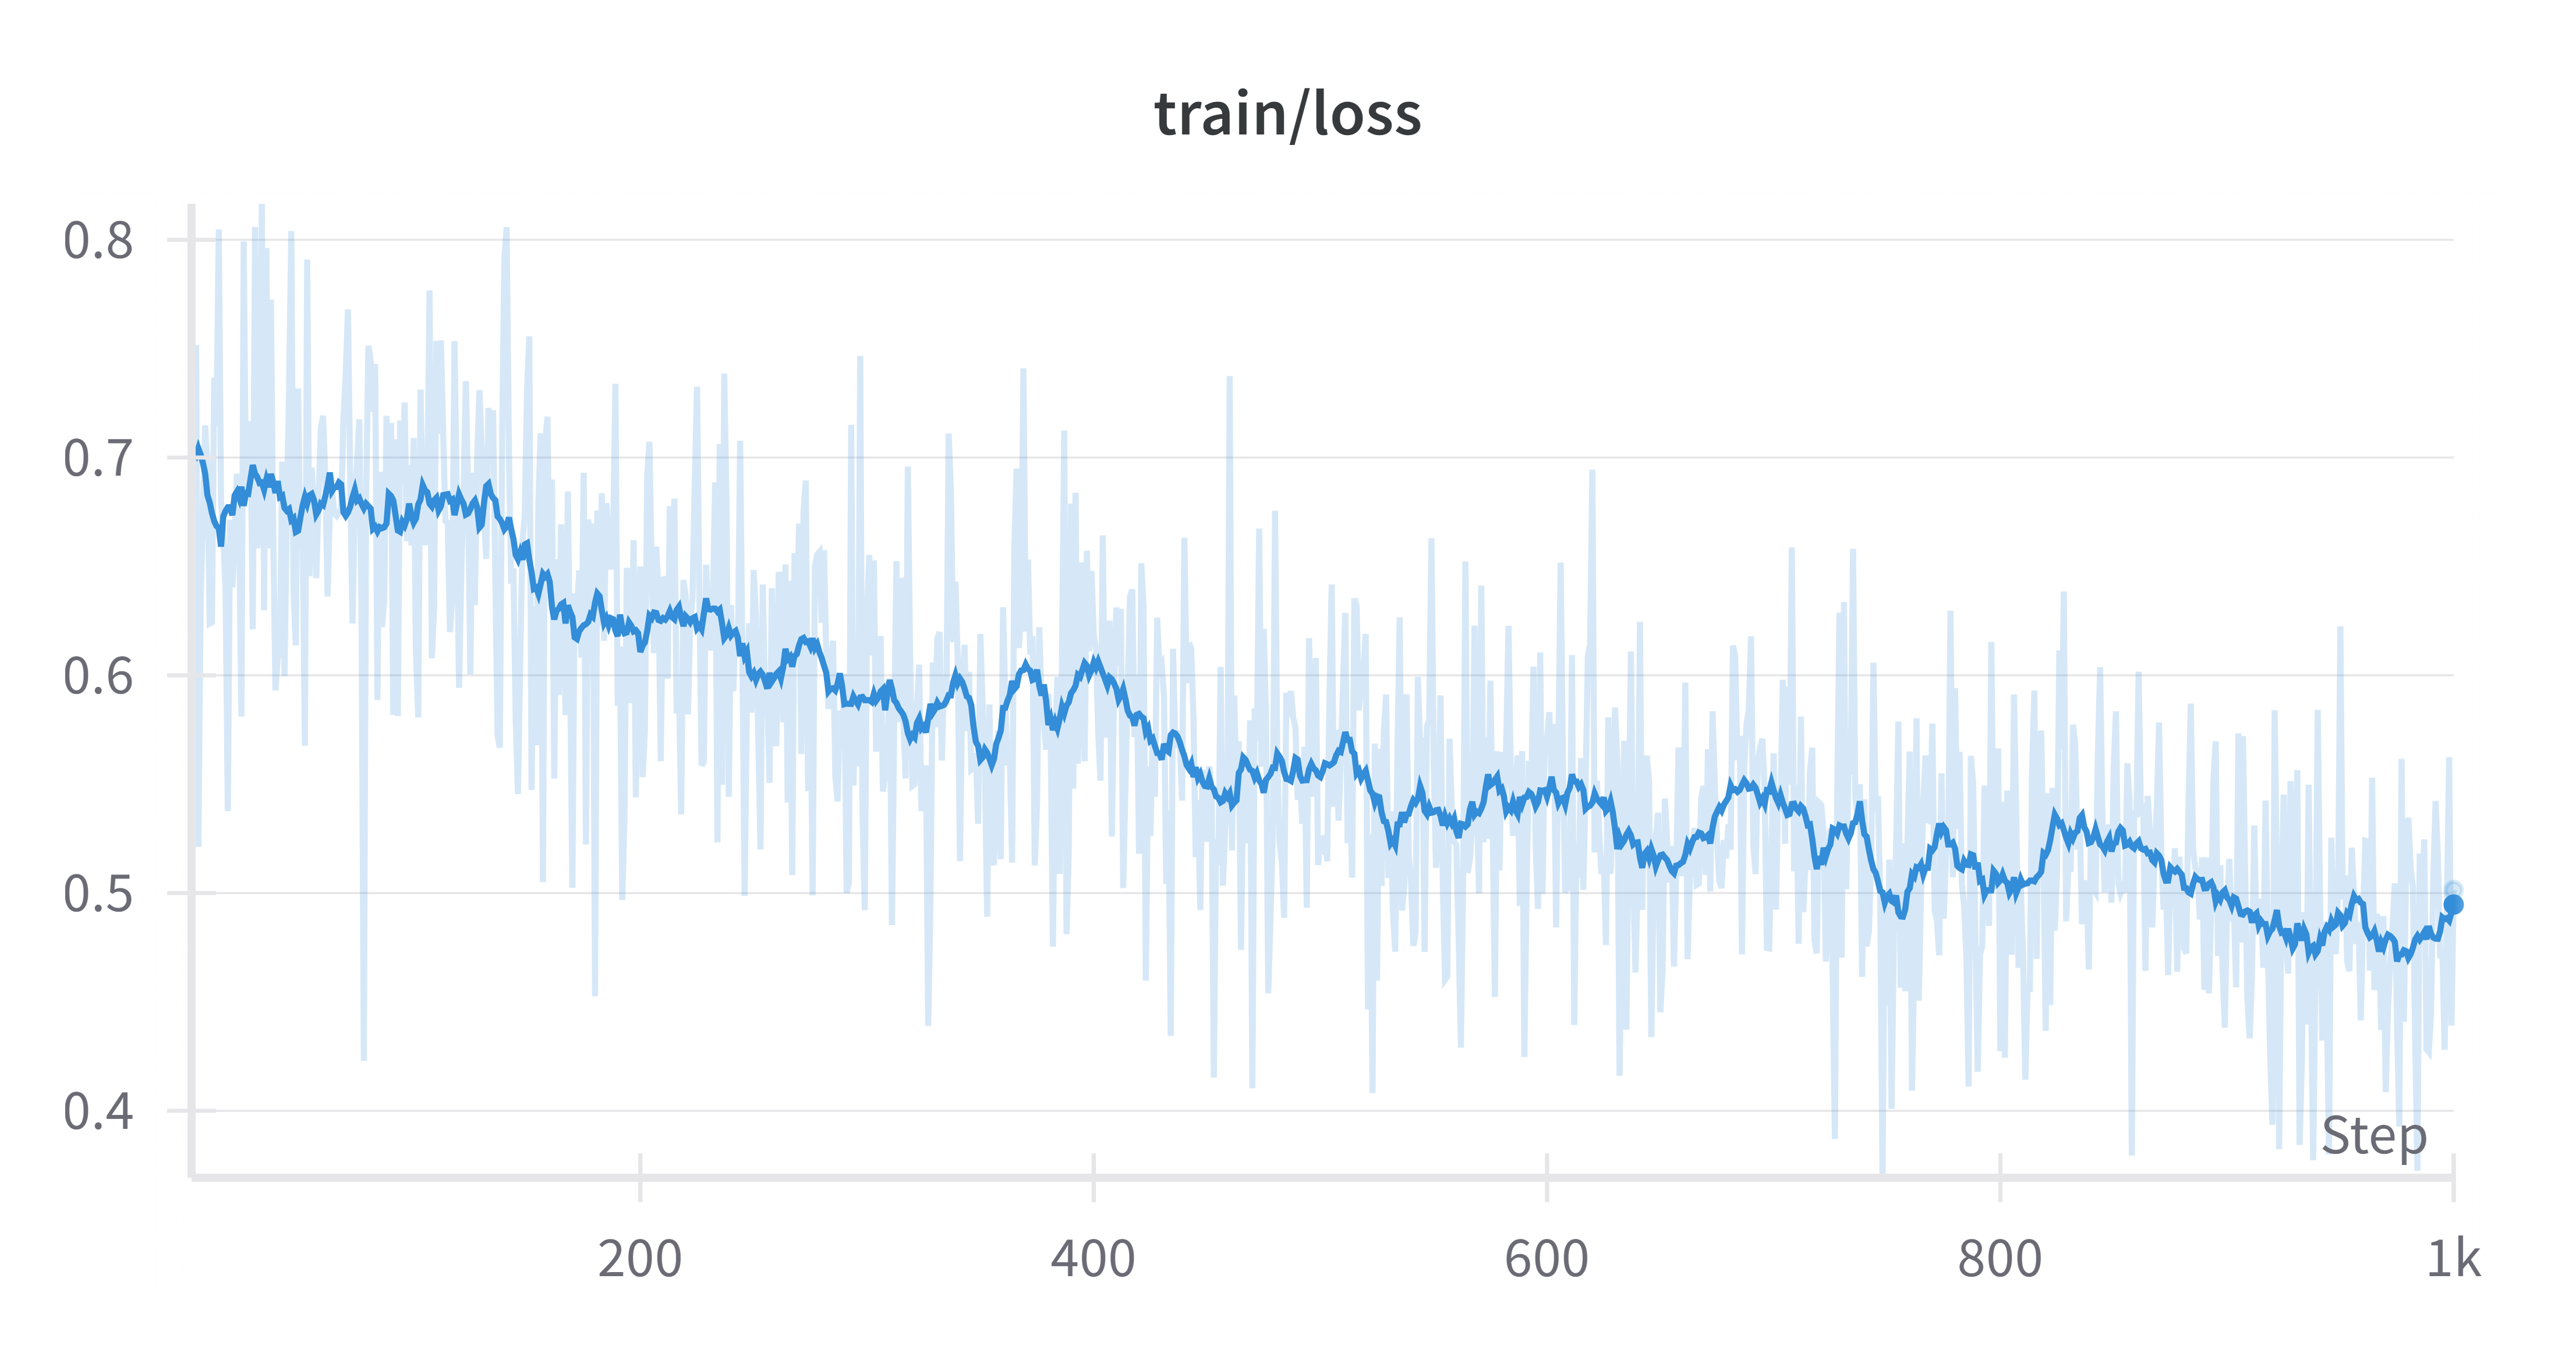
\includegraphics[width=\linewidth]{M2 Course Work//Images/initial_train_loss.png}
        \caption{Training Loss} \label{fig:initial_train_loss}
    \end{subfigure} \hfill
    \begin{subfigure}[b]{0.48\linewidth} \centering
        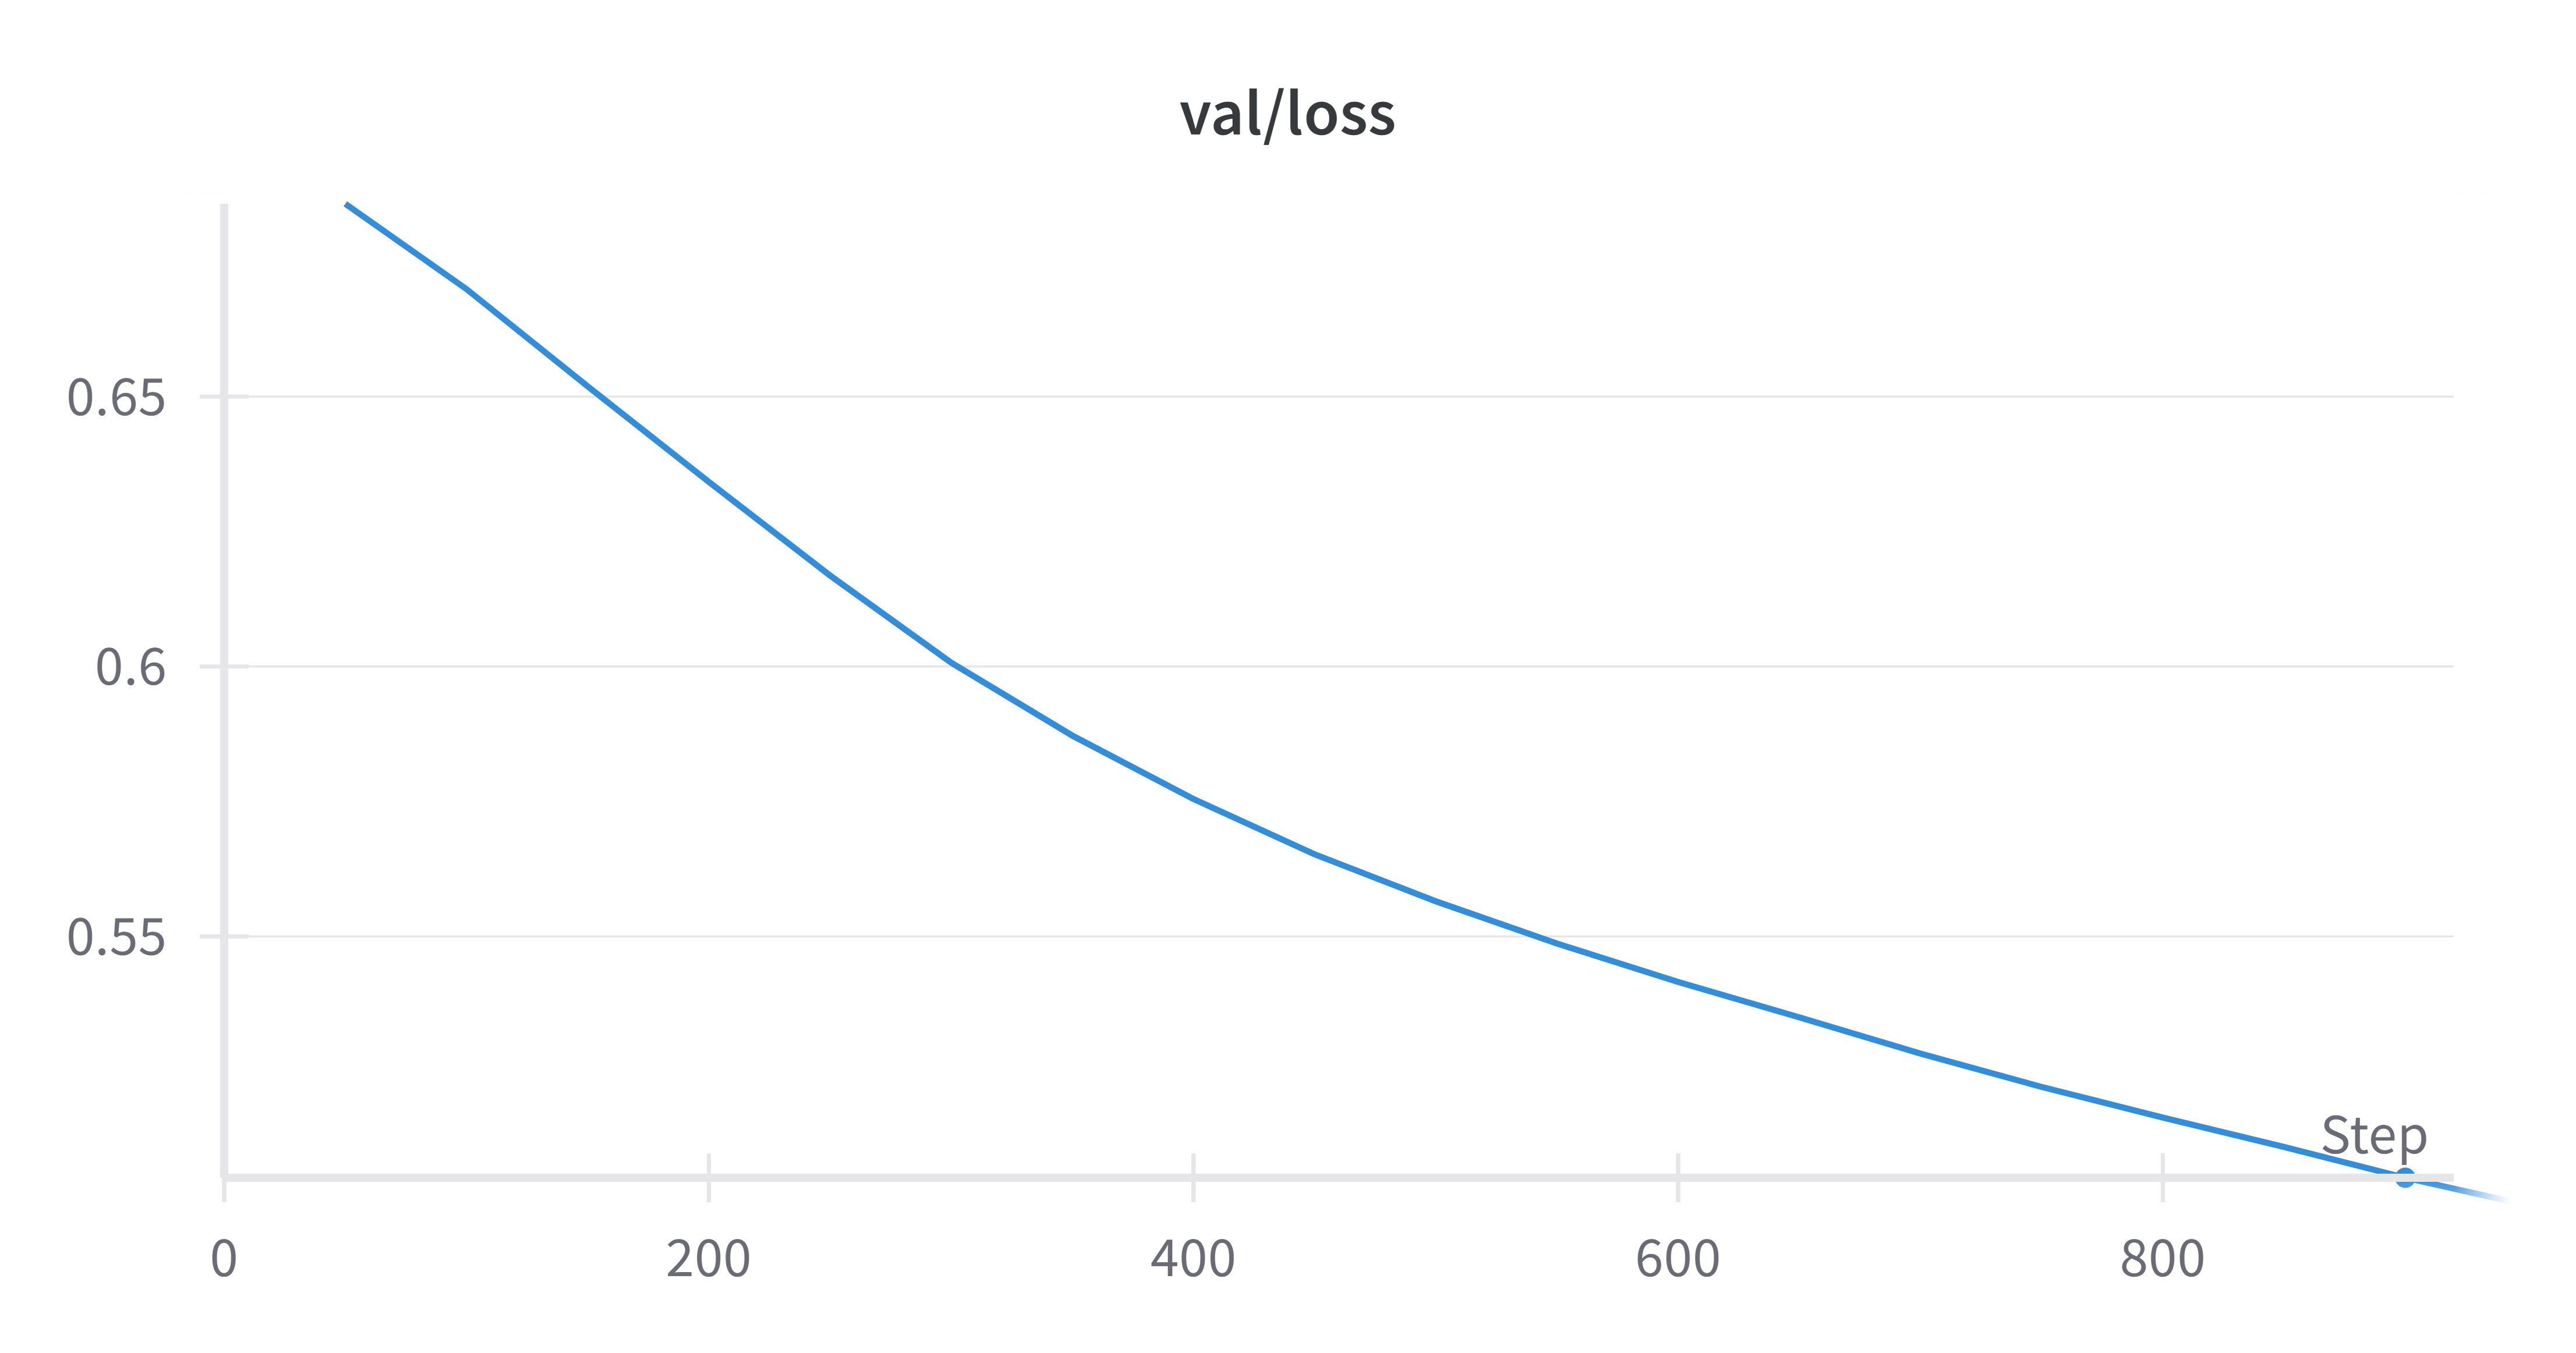
\includegraphics[width=\linewidth]{M2 Course Work//Images/initial_validation_loss.png}
        \caption{Validation Loss} \label{fig:initial_valid_loss}
    \end{subfigure}
    \caption{Loss curves during initial 1000 steps of fine-tuning (default hyperparameters).} % Shortened caption
    \label{fig:initial_loss_curves}
\end{figure}

Both the training and validation losses decreased consistently (Figure \ref{fig:initial_loss_curves}), indicating successful learning. Test set performance improved dramatically compared to the baseline (Table \ref{tab:training_stage_comparison}, Initial Training), with MSE and MAE reducing significantly for the trained context length ($S=512$) and also showing improvement when evaluated on other context lengths ($S=128, S=768$). Predictions (Figure \ref{fig:initial_training_predictions} in Appendix) now attempted to follow the cyclical patterns, producing curved trajectories instead of flat lines, although deviations in phase/amplitude remained, especially over longer horizons. This demonstrated the potential of LoRA fine-tuning.




\subsection{Hyper-parameter Search (Q3b)}

To optimize performance, we conducted searches over key hyper-parameters, training each configuration for 500 steps.

\paragraph{Learning Rate and LoRA Rank}
A grid search explored learning rates $\eta \in \{10^{-5}, 5 \times 10^{-5}, 10^{-4}\}$ and LoRA ranks $r \in \{2, 4, 8\}$ at fixed $S=512$. Loss curves generally showed decreasing and good learning dynamics (Figure \ref{fig:grid_search_lr_rank_loss_curves}). Comparing validation MAE (Figure \ref{fig:grid_search_lr_rank_results}), the best performance was achieved with the highest learning rate ($\eta=10^{-4}$) and highest rank ($r=8$) tested. This suggests that adapting from language to time-series, a significant change in domain, benefits from larger parameter updates (higher $\eta$) and increased adaptation capacity (higher $r$).
% Therefore, we selected $\eta=10^{-4}$ and $r=8$ going forward.

% Keep Figure: Grid Search LR/Rank Loss (Optional: could remove if space is tight and text summary suffices)
\begin{figure}[!htbp]
    \centering
    \begin{subfigure}[b]{0.48\linewidth} \centering
        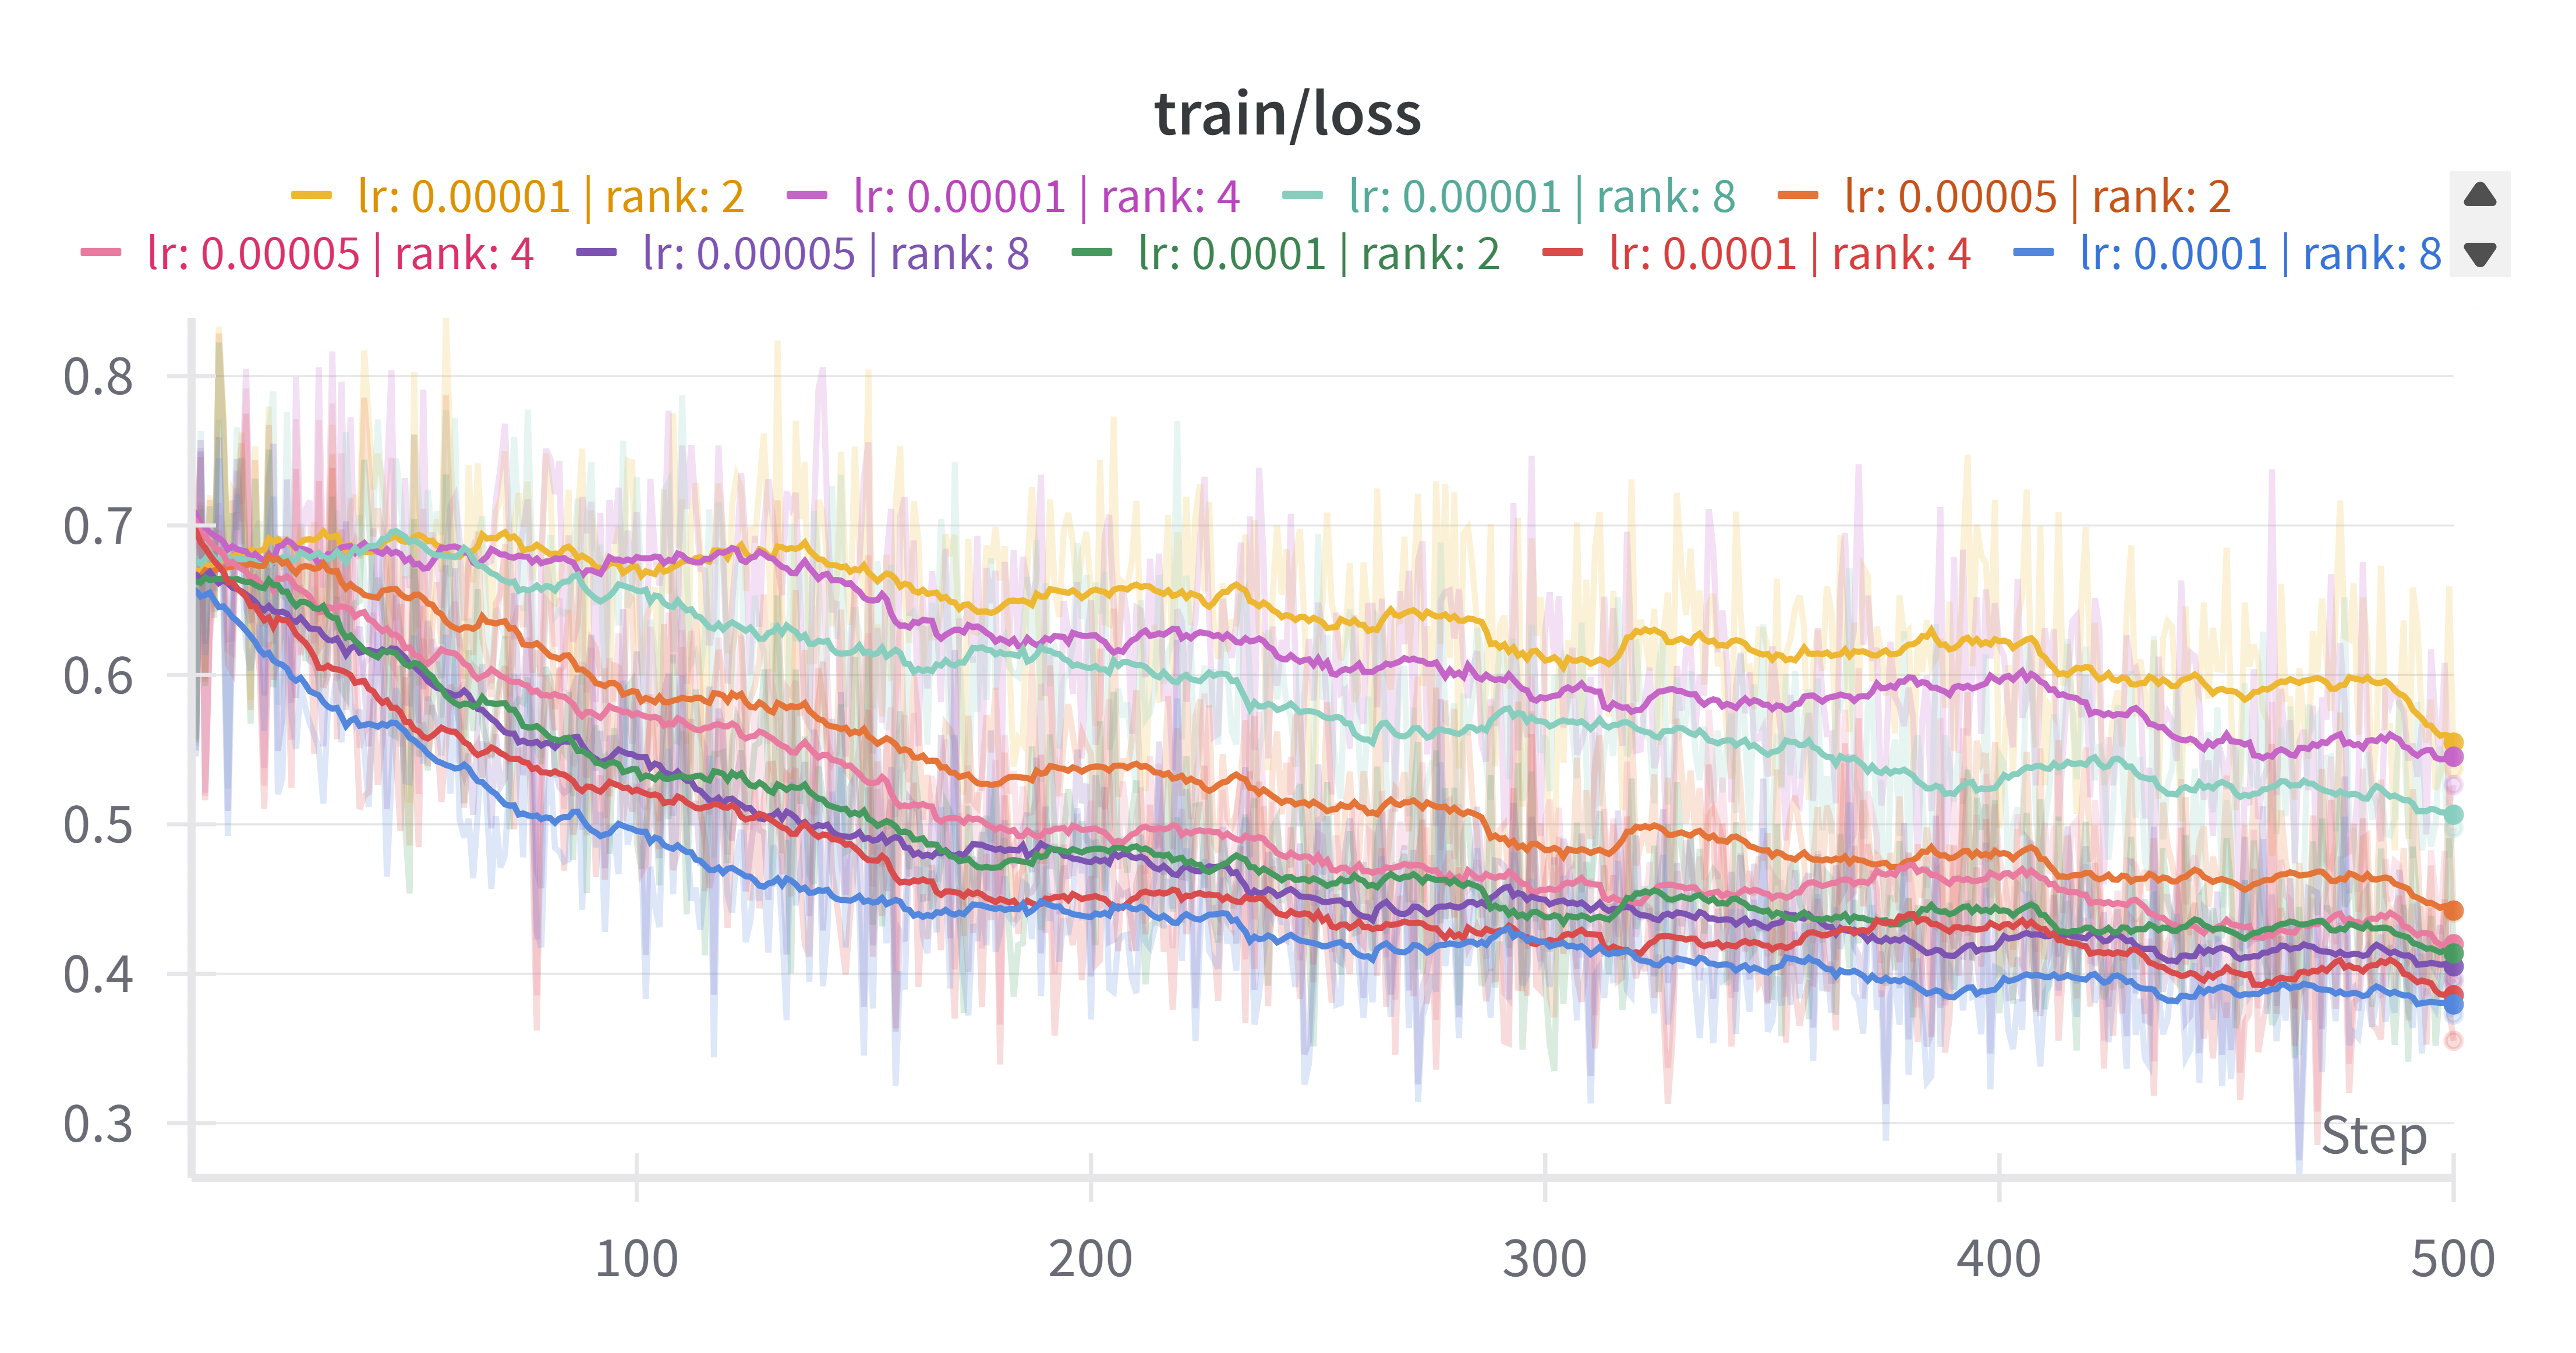
\includegraphics[width=\linewidth]{M2 Course Work//Images/grid_search_training_loss.png}
        \caption{Training Loss} \label{fig:grid_search_lr_rank_train_loss}
    \end{subfigure} \hfill
    \begin{subfigure}[b]{0.48\linewidth} \centering
        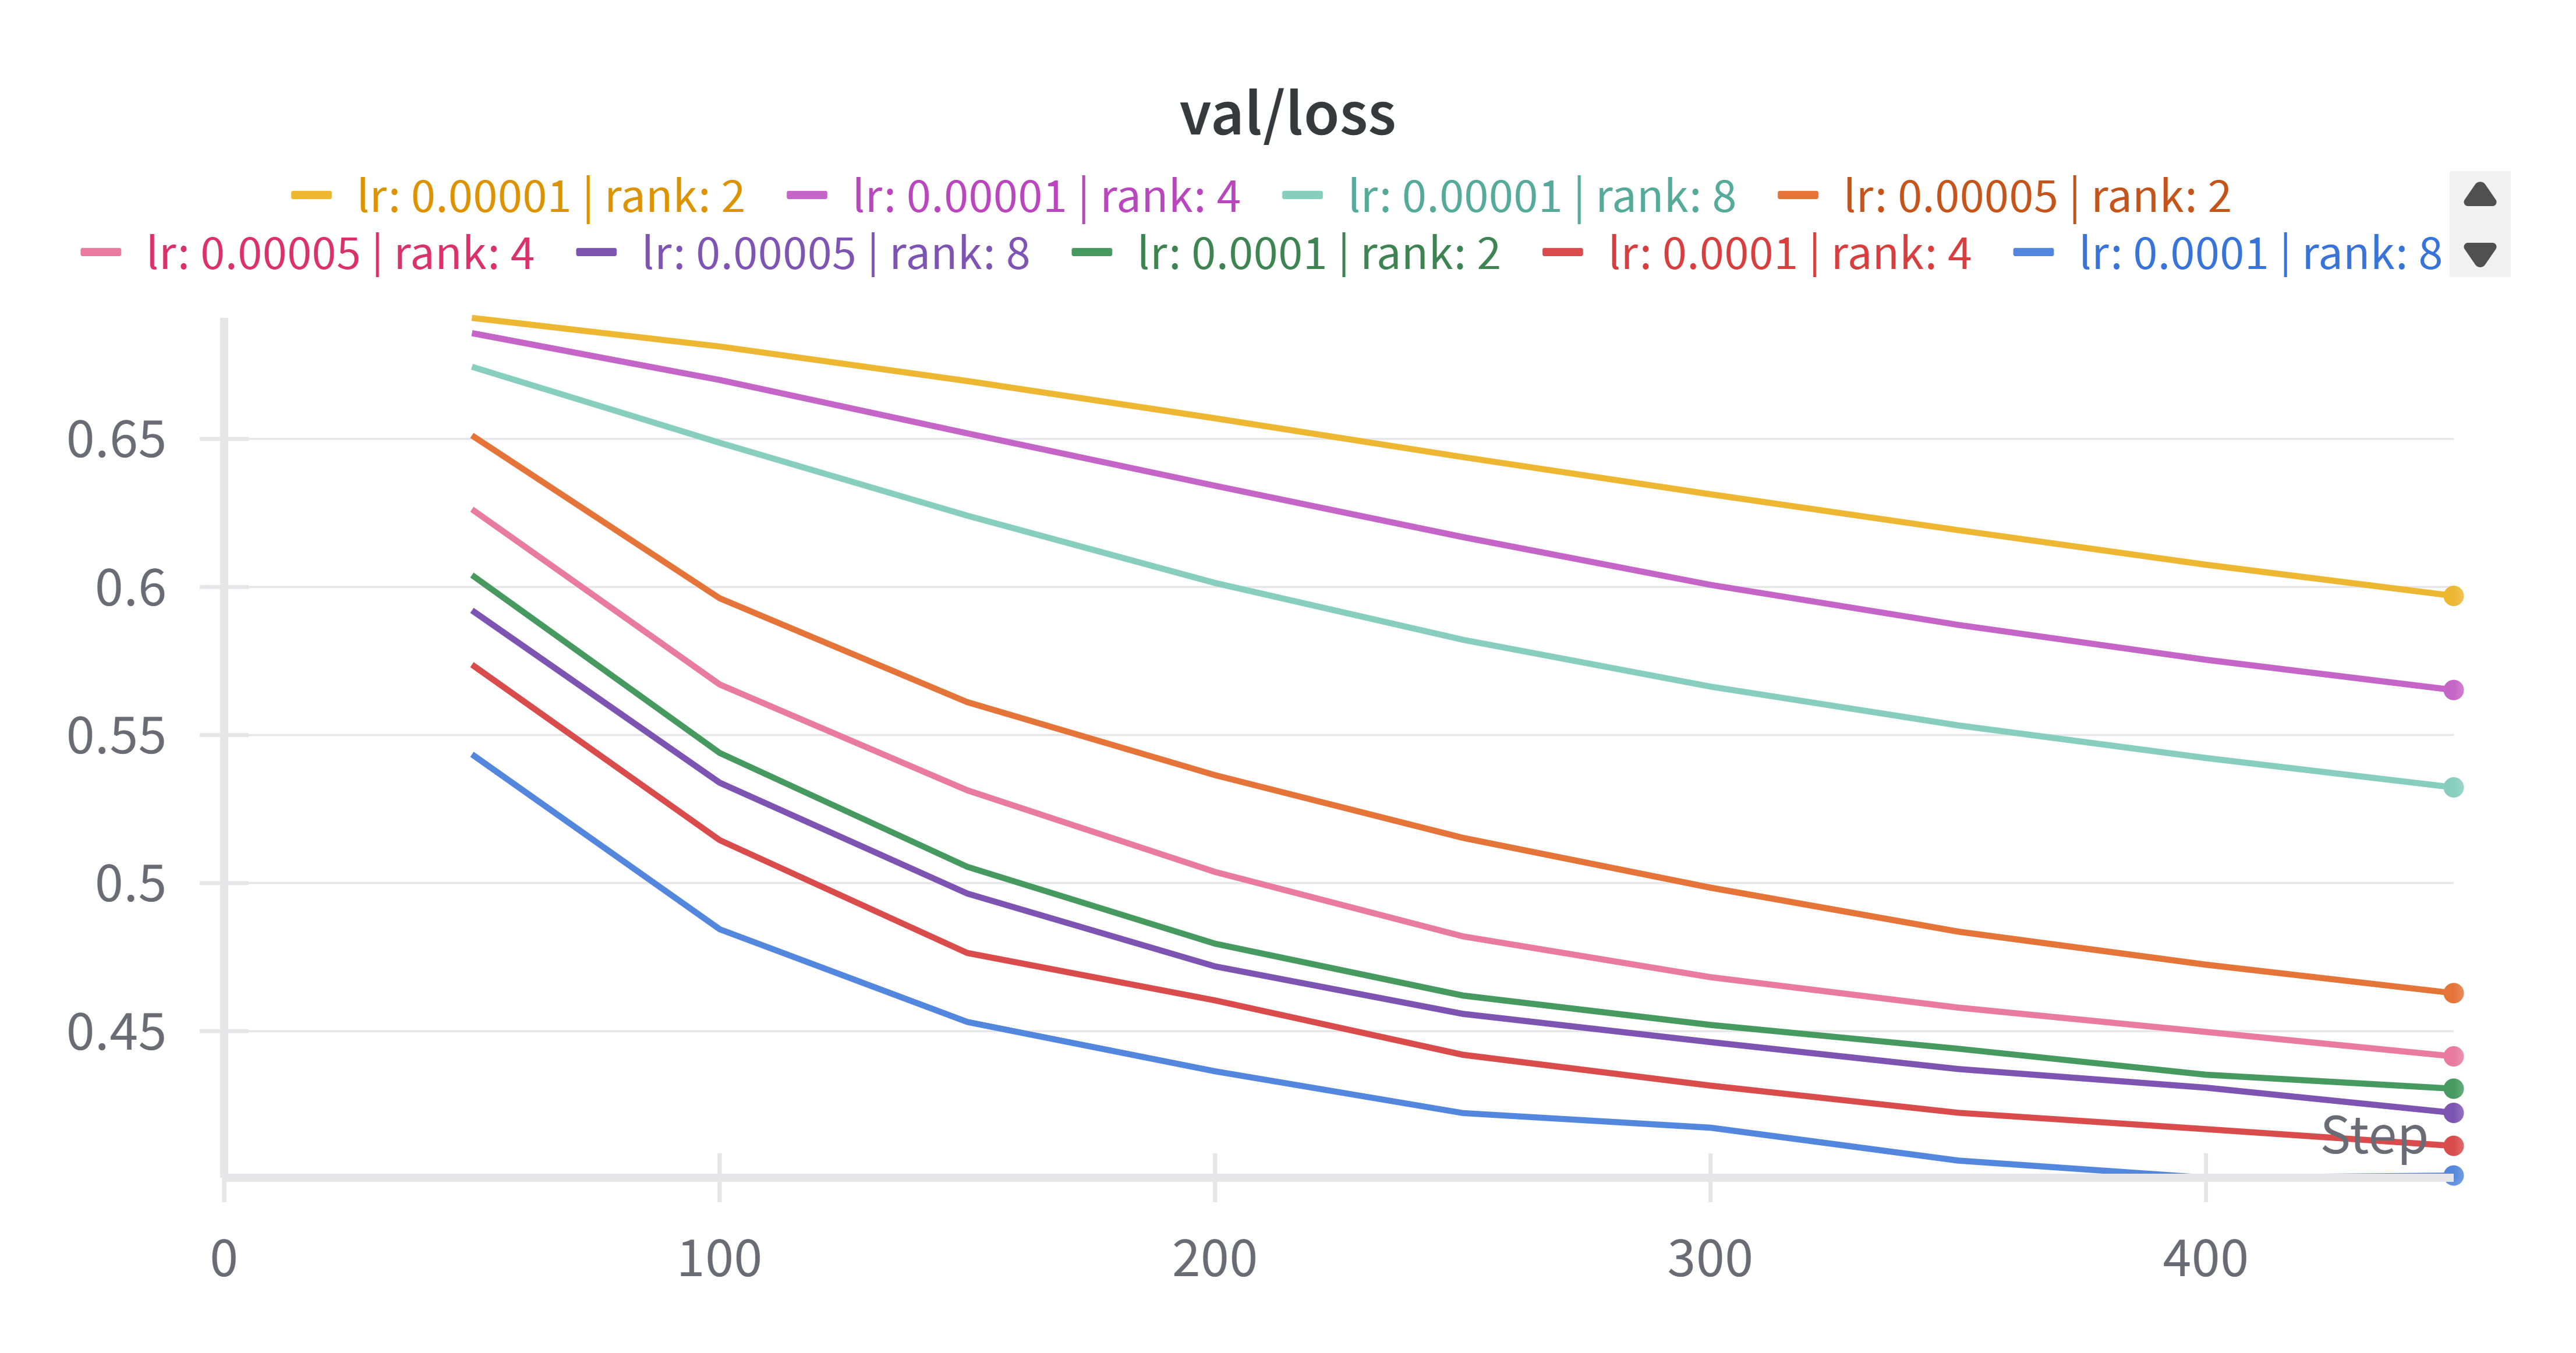
\includegraphics[width=\linewidth]{M2 Course Work//Images/grid_search_validiation_loss.png}
        \caption{Validation Loss} \label{fig:grid_search_lr_rank_valid_loss}
    \end{subfigure}
    \caption{Loss curves from grid search over learning rate ($\eta$) and LoRA rank ($r$).} % Shortened caption
    \label{fig:grid_search_lr_rank_loss_curves}
\end{figure}

% Keep Figure: Grid Search LR/Rank Results
\begin{figure}[!htbp]
    \centering
    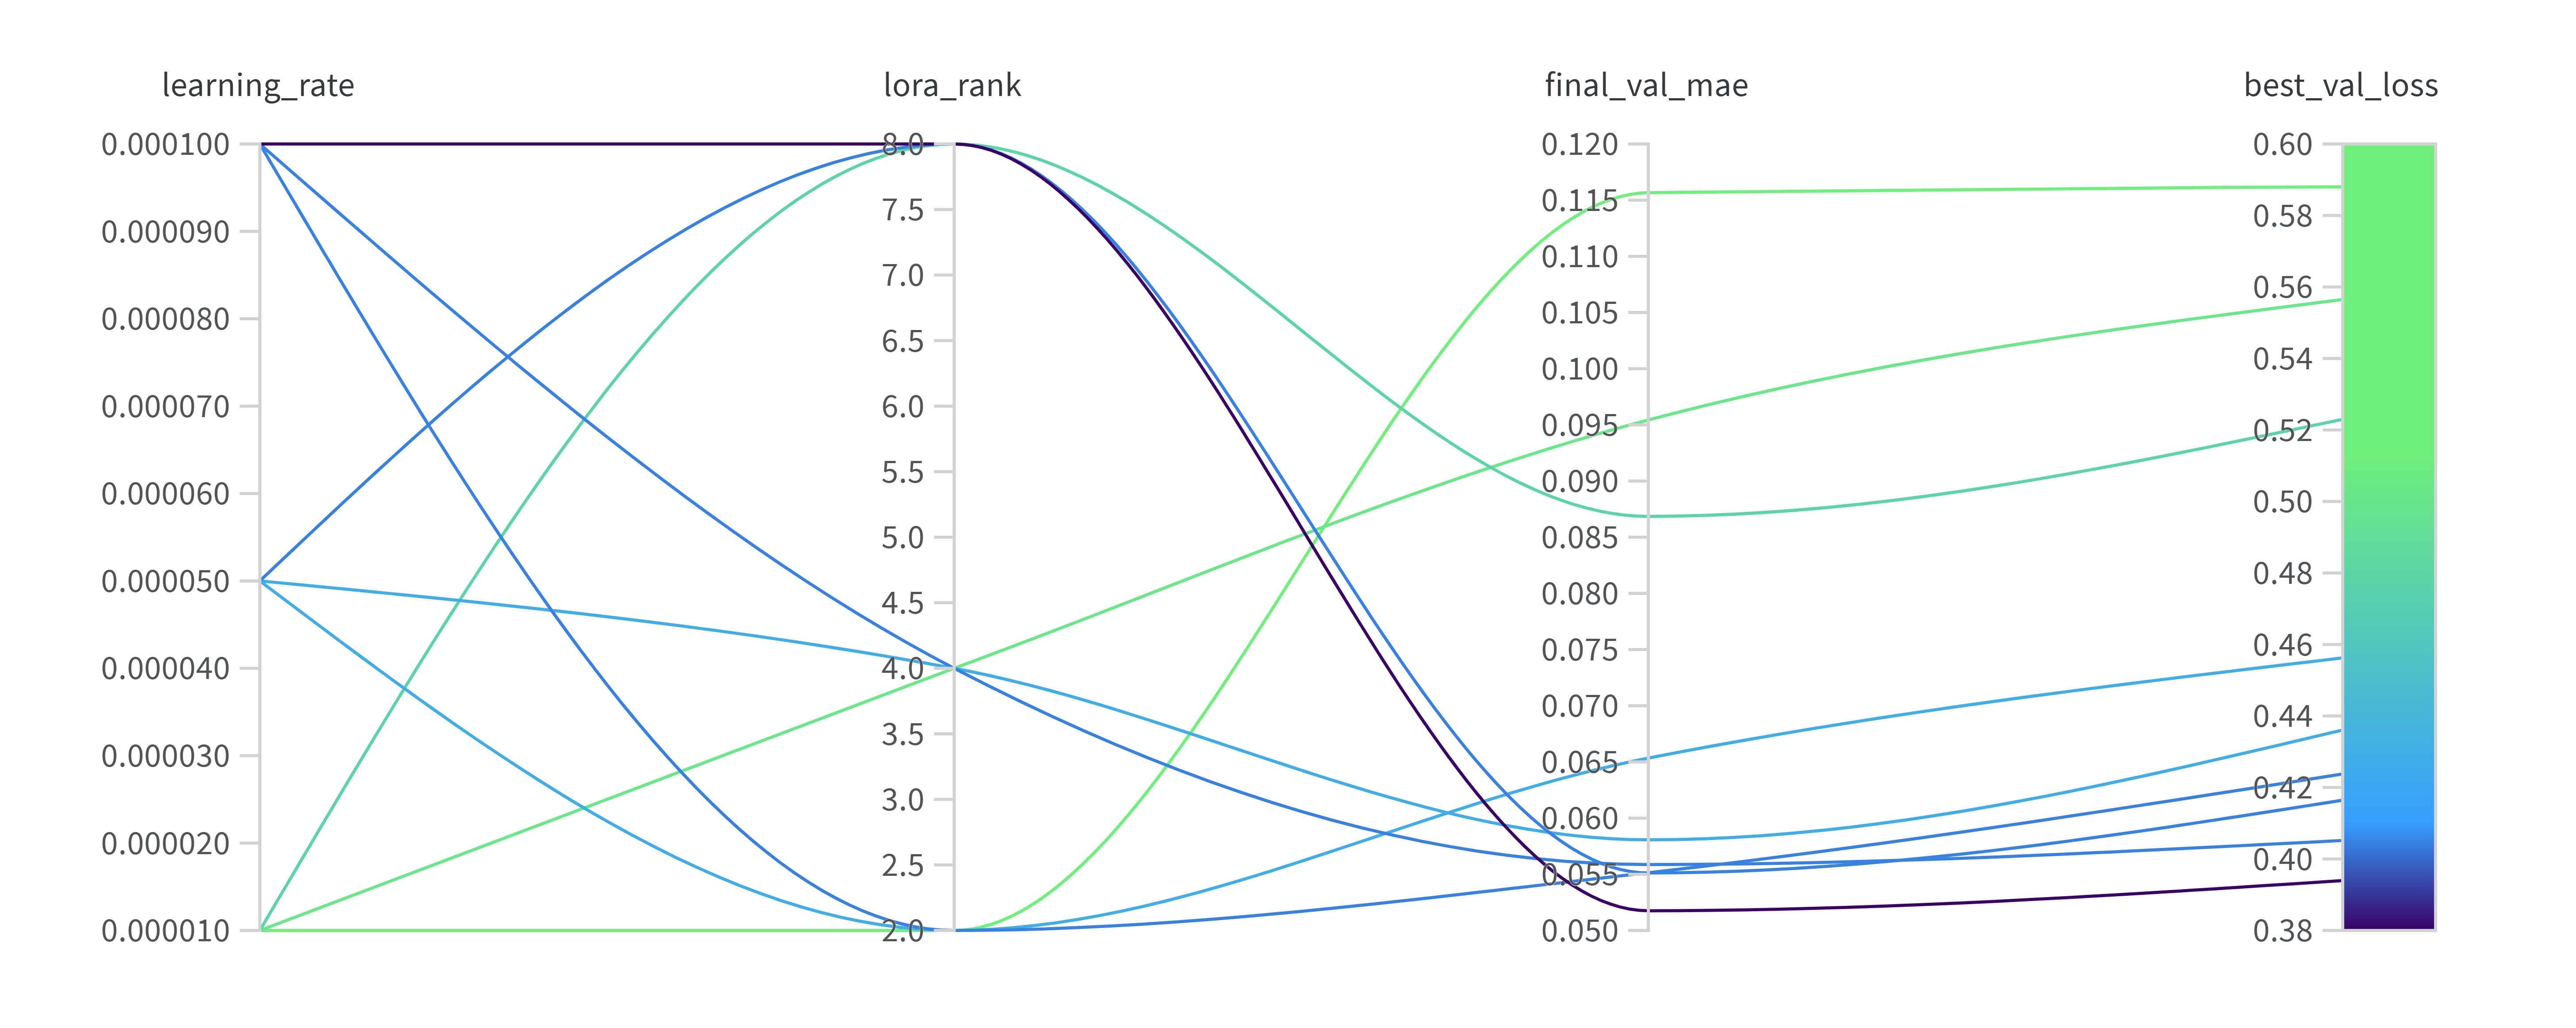
\includegraphics[width=0.6\linewidth]{M2 Course Work//Images/grid_search_result.png}
    \caption{Validation MAE after 500 steps for varying LoRA rank ($r$) and learning rate ($\eta$) at $S=512$. Lower is better. Best: $r=8, \eta=10^{-4}$.} % Shortened caption
    \label{fig:grid_search_lr_rank_results}
\end{figure}

\paragraph{Context Length}
Using the best $\eta=10^{-4}$ and $r=8$, we evaluated context lengths $S \in \{128, 512, 768\}$. Loss curves are shown in Figure \ref{fig:context_search_loss_curves}. Comparing validation MAE (Figure \ref{fig:context_search_results}), performance consistently improved with longer context lengths. The lowest MAE was achieved with $S=768$, confirming that providing more historical information aids prediction accuracy. 
% We selected $S=768$ going forward.

% Keep Figure: Context Search Loss (Optional: could remove if space is tight)
\begin{figure}[!htbp]
    \centering
    \begin{subfigure}[b]{0.48\linewidth} \centering
        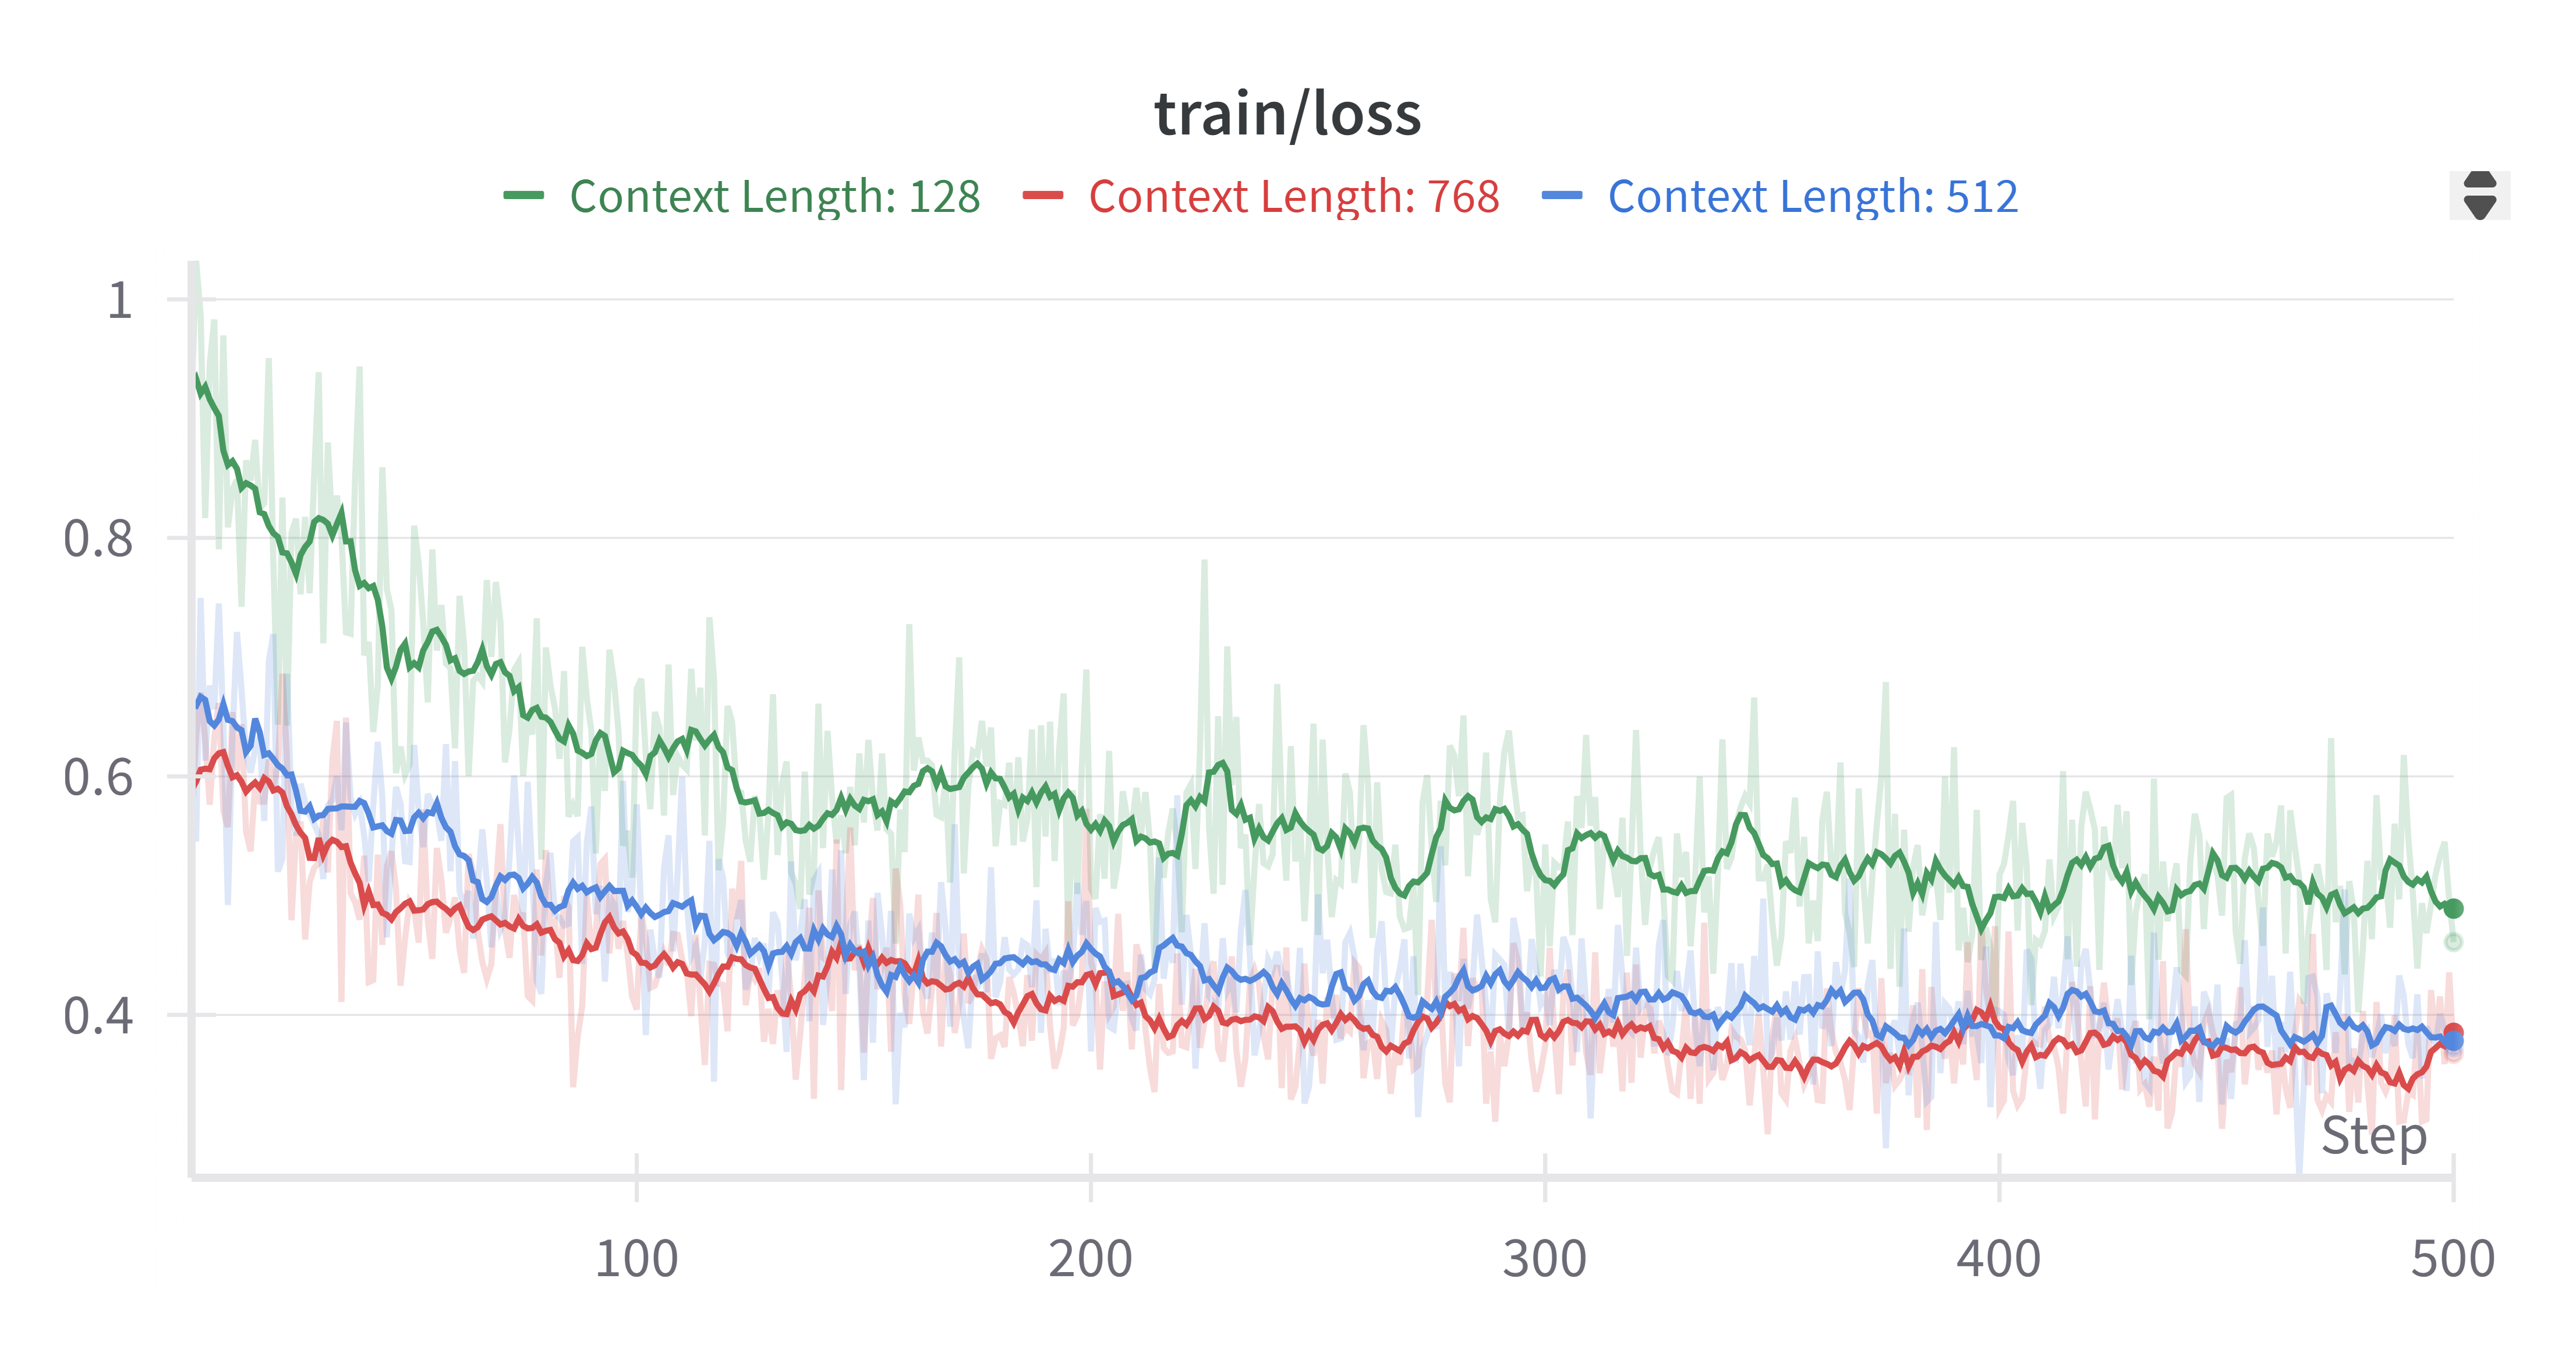
\includegraphics[width=\linewidth]{M2 Course Work/Images/sweep_context_length_training.png}
        \caption{Training Loss} \label{fig:context_search_train_loss}
    \end{subfigure} \hfill
    \begin{subfigure}[b]{0.48\linewidth} \centering
        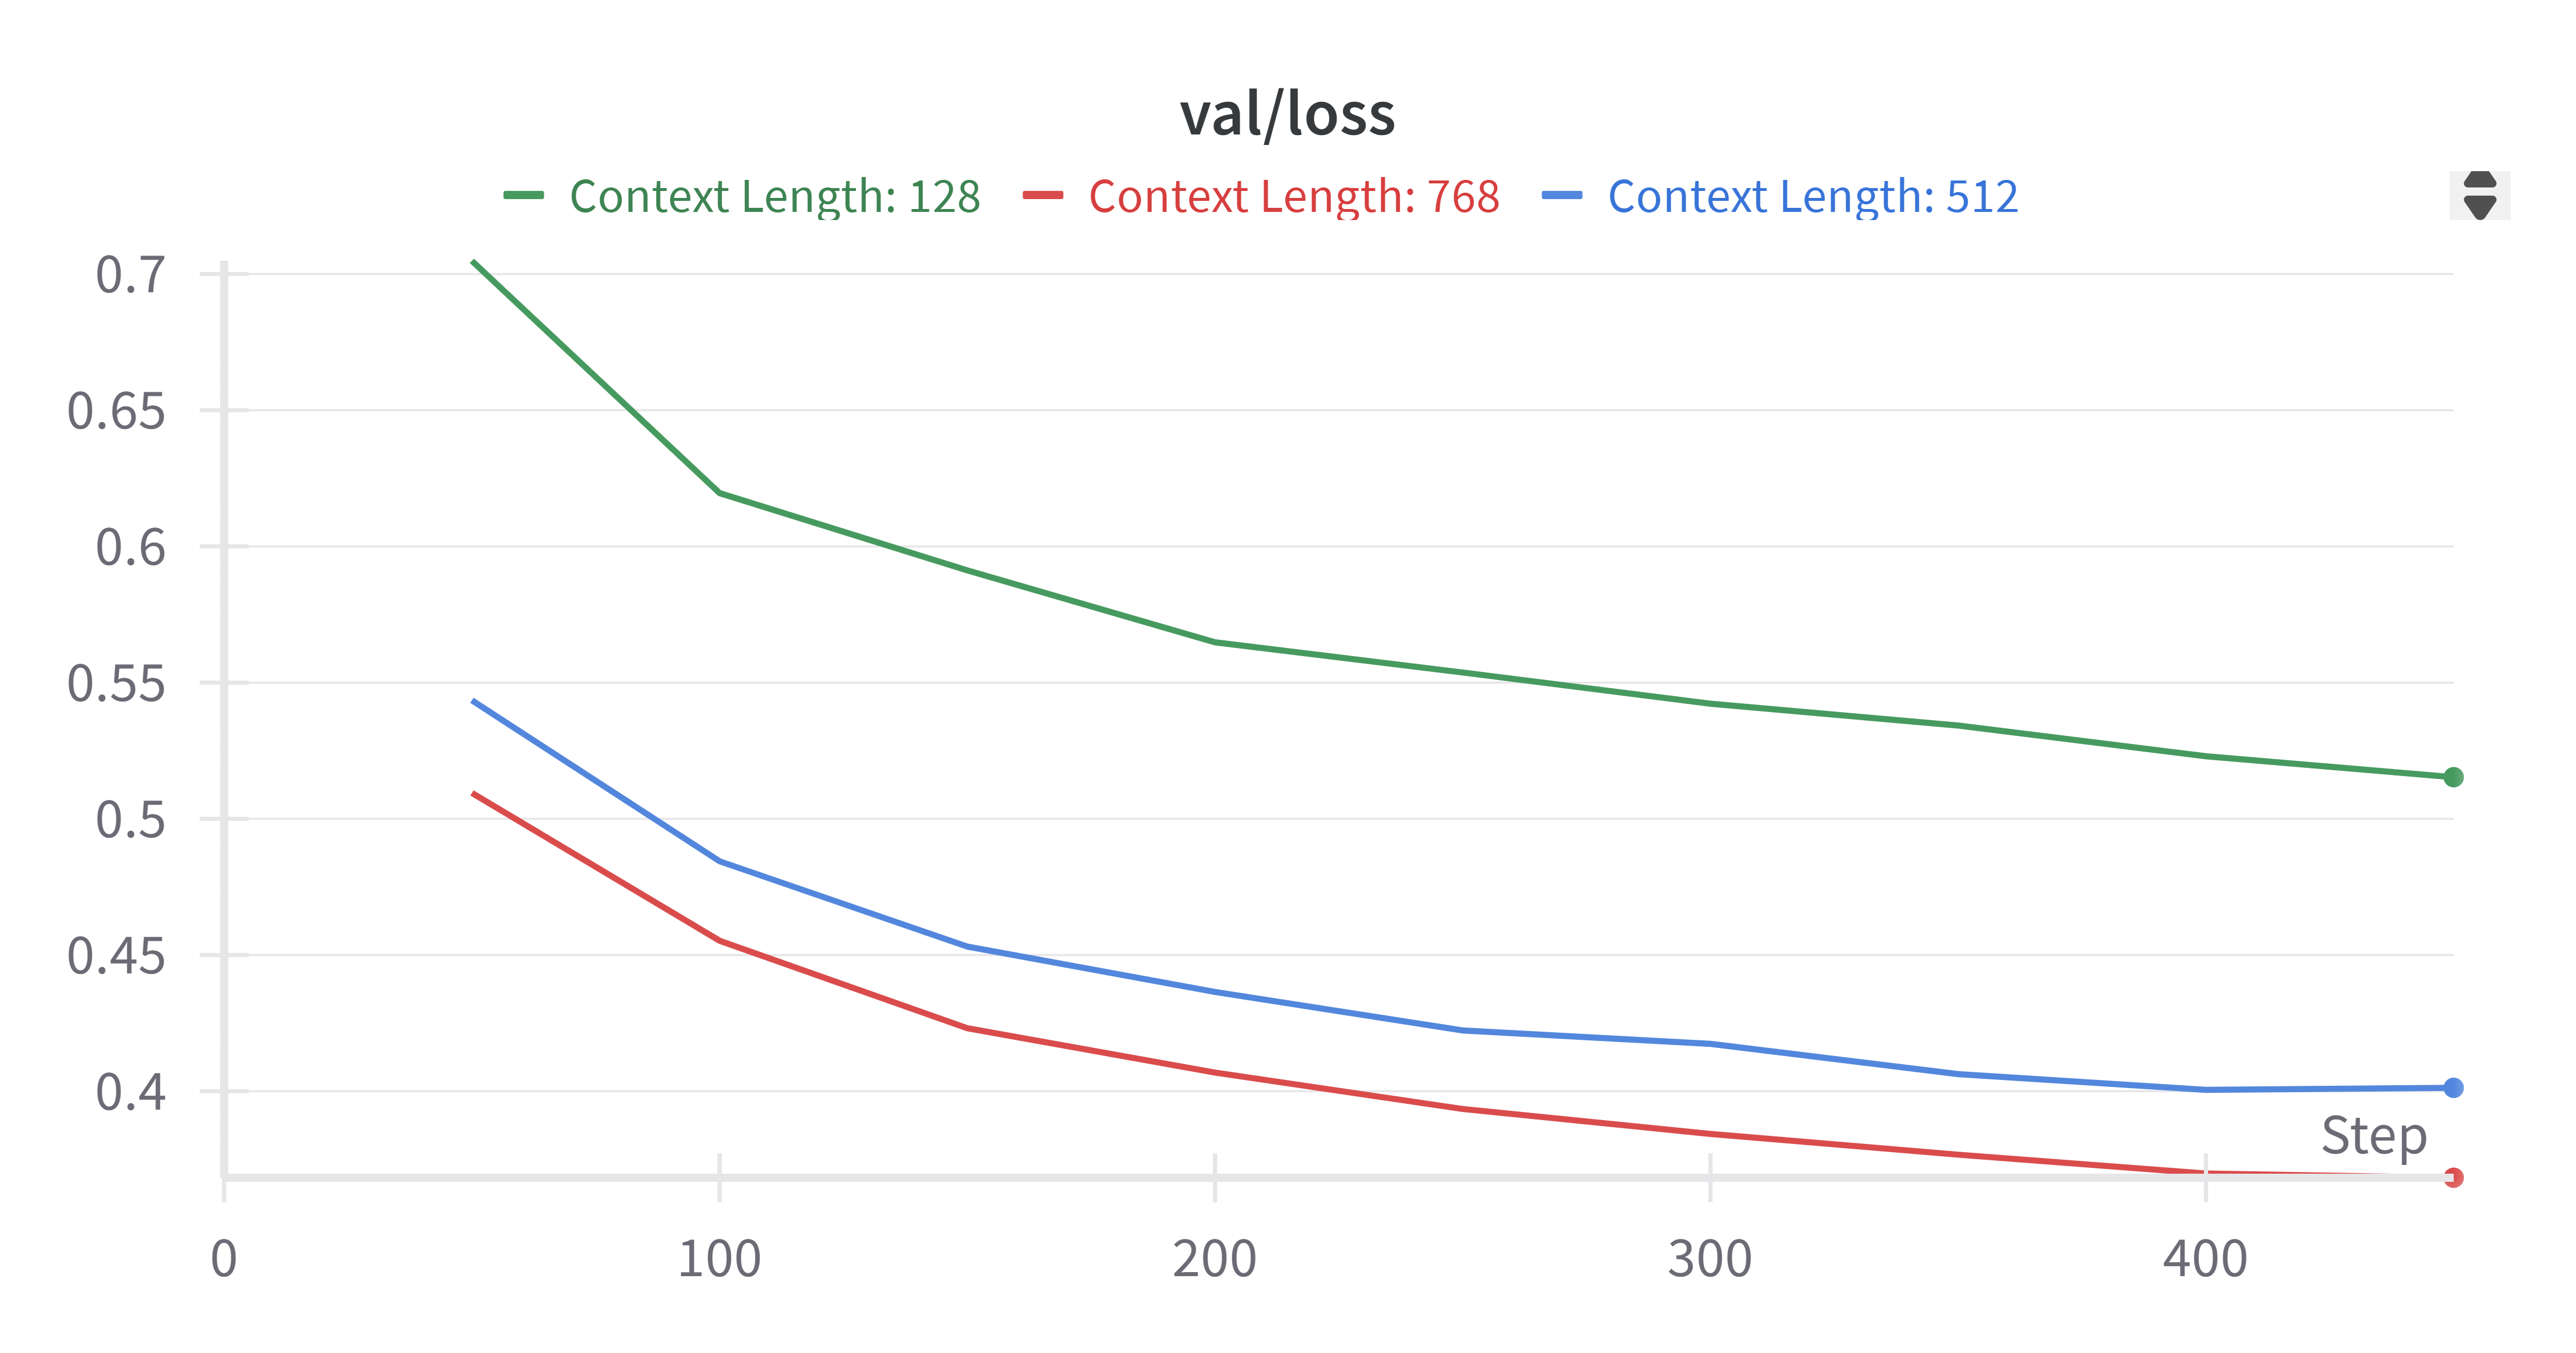
\includegraphics[width=\linewidth]{M2 Course Work/Images/sweep_context_length_validation.png}
        \caption{Validation Loss} \label{fig:context_search_valid_loss}
    \end{subfigure}
    \caption{Loss curves for different context lengths ($S$) using best $\eta, r$.} % Shortened caption
    \label{fig:context_search_loss_curves}
\end{figure}

% Keep Figure: Context Search Results
\begin{figure}[!htbp]
    \centering
    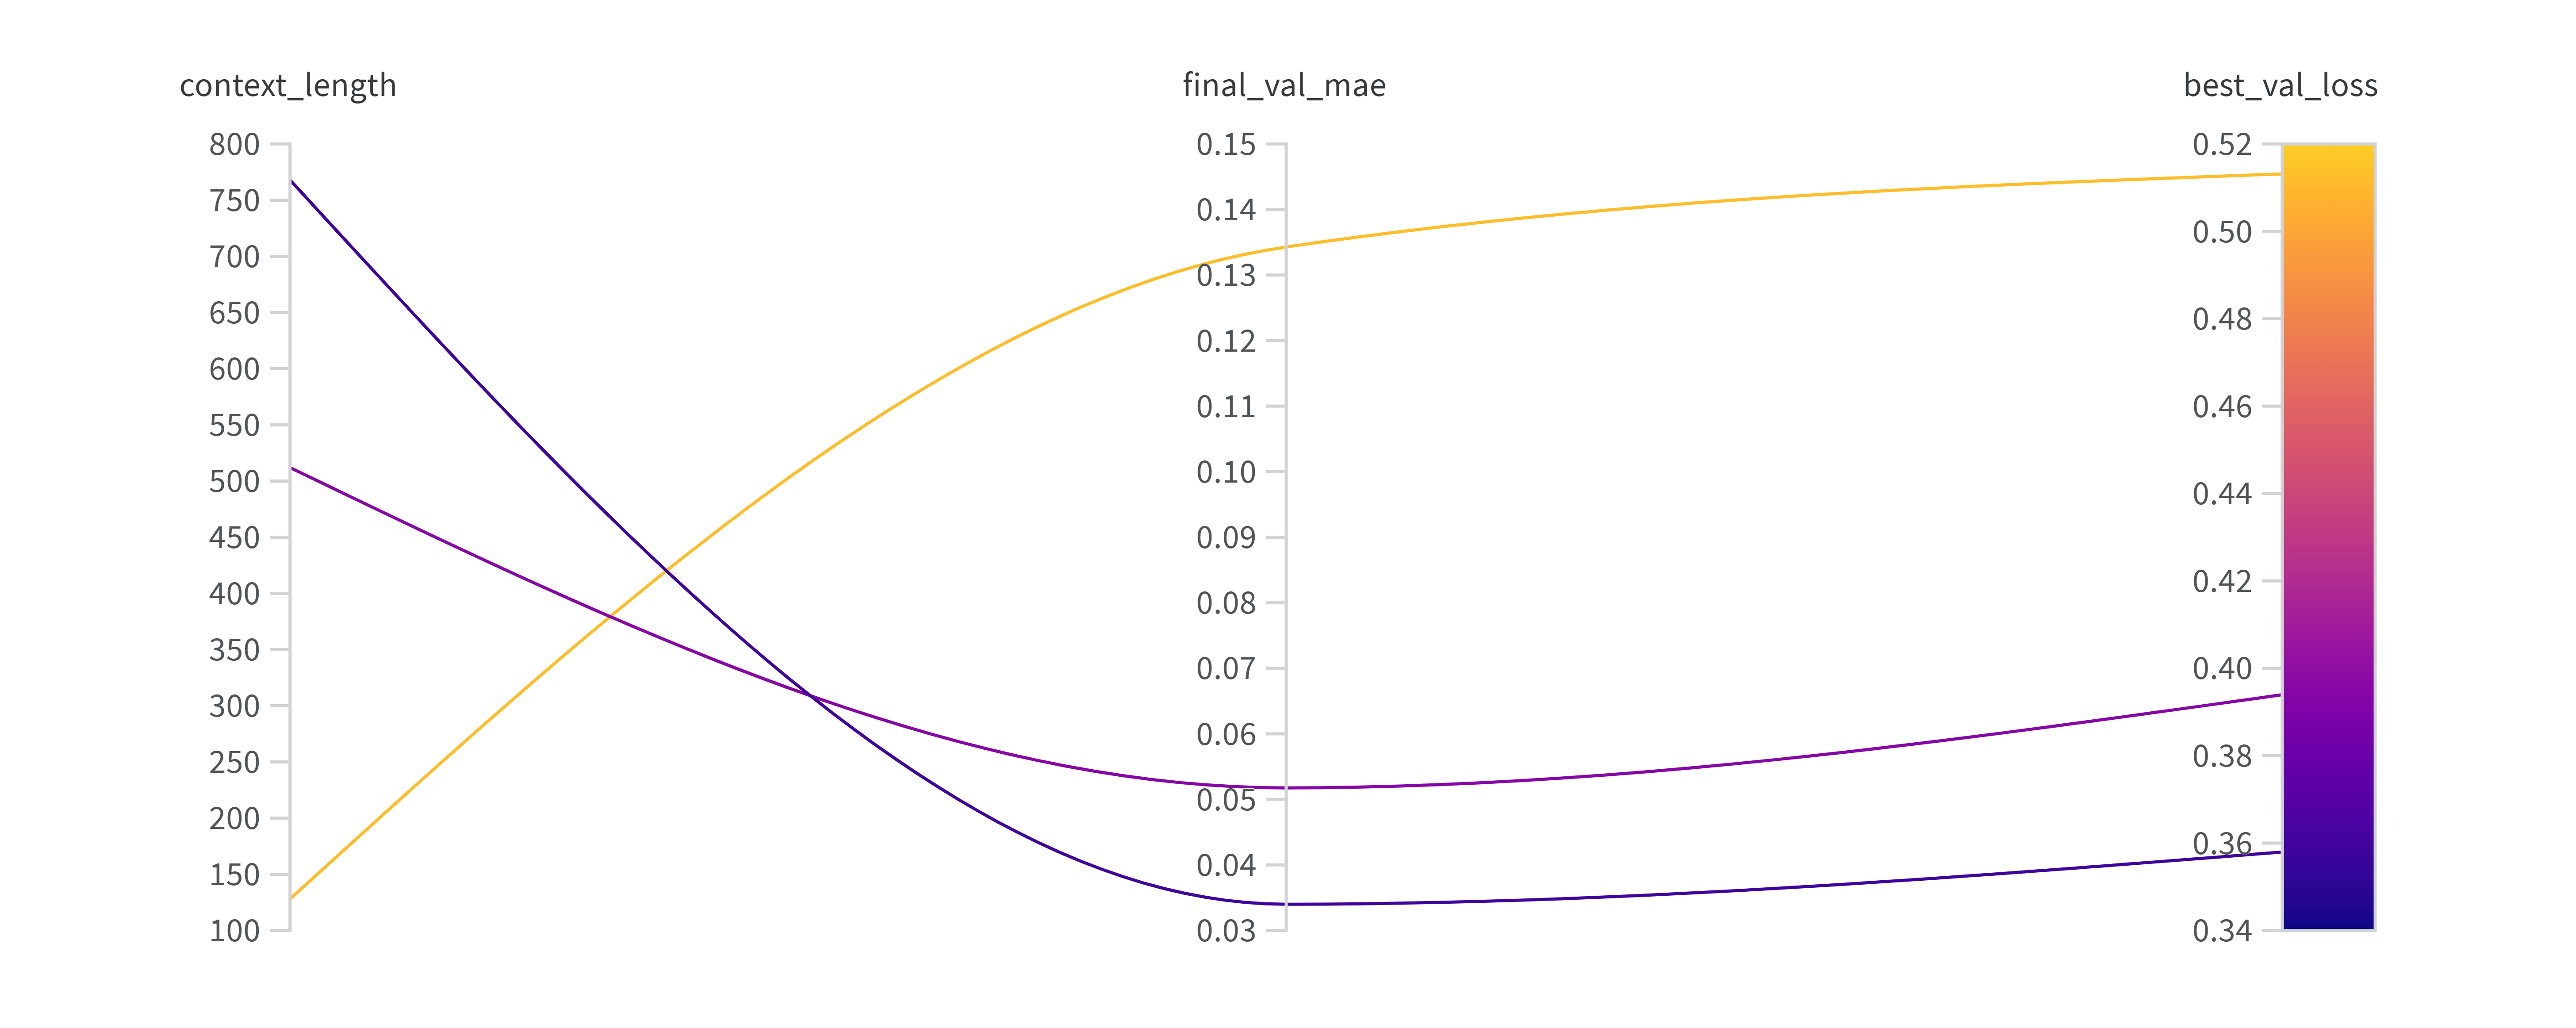
\includegraphics[width=0.6\linewidth]{M2 Course Work//Images/sweep_context_length_result.png}
    \caption{Validation MAE after 500 steps for different context lengths ($S$) using best $\eta, r$. Lower is better. Best: $S=768$.} % Shortened caption
    \label{fig:context_search_results}
\end{figure}


\begin{table}[!h]
\renewcommand{\arraystretch}{1.4}
\centering
\setlength{\tabcolsep}{8pt} % Adjust column separation if needed
\sisetup{round-mode=places, round-precision=5} % Keep precision for final value
\begin{tabular}{lcccrS[round-precision=6]} % l for Sweep Type, c for context, r for rank, S for numbers
    \toprule
    \textbf{Sweep Type} & \textbf{Context Length} & \textbf{Learning Rate} & {\textbf{Rank}} & {\textbf{Validation MAE}} \\ % Use braces to protect header text in S columns
    \midrule
    Rank and LR Sweep   & 512 & 1e-5 & 2 & 0.11567  \\
    Rank and LR Sweep   & 512 & 1e-5 & 4 & 0.095438 \\
    Rank and LR Sweep   & 512 & 1e-5 & 8 & 0.086855 \\
    Rank and LR Sweep   & 512 & 5e-5 & 2 & 0.065344 \\
    Rank and LR Sweep   & 512 & 5e-5 & 4 & 0.058066 \\
    Rank and LR Sweep   & 512 & 5e-5 & 8 & 0.055118 \\
    Rank and LR Sweep   & 512 & 1e-4 & 2 & 0.055142 \\ % Note: Repeated condition? Maybe different run?
    Rank and LR Sweep   & 512 & 1e-4 & 4 & 0.055869 \\ % Note: Repeated condition? Maybe different run?
    Rank and LR Sweep   & 512 & 1e-4 & 8 & 0.051754 \\ % Note: Repeated condition? Maybe different run?
    \midrule % Added a rule to visually separate the sweep types
    Context Length Sweep& 128 & 1e-4 & 8 & 0.13428  \\
    Context Length Sweep& 512 & 1e-4 & 8 & 0.051754 \\
    Context Length Sweep& 768 & 1e-4 & 8 & 0.034004 \\
    \bottomrule
\end{tabular}
\caption{Hyperparameter Tuning Results: Final Validation MAE for Different LoRA Ranks, Learning Rates, and Context Lengths, Organized by Sweep Strategy.}
\label{tab:experiment_results_by_sweep} % Adjusted label
\end{table}




\subsection{Final Training with Optimal Configuration (Q3c)}
\label{sec:final}
The final model was trained using the optimized hyper-parameters: $\eta=10^{-4}, r=8, S=768$. Training utilized the remaining FLOPS budget $40\%$, running for approximately 3000 steps. The loss curves (Figure \ref{fig:final_training_loss_curves}) show steady initial improvement, with the validation loss starting to plateau towards the end, suggesting convergence near the allocated budget limit.

Test set evaluation (Table \ref{tab:training_stage_comparison}, Final Training) reveals substantial improvement over the initial training phase. For the optimal $S=768$, MSE improved by over an order of magnitude, reaching $0.0020$, and MAE reached $0.0191$. This final MAE is somewhat close to the estimated information loss from the LLMTime preprocessing (Table \ref{tab:round_trip_test}), indicating the model learned the patterns nearly as well as possible given the data representation. Final predictions (Figure \ref{fig:final_training_predictions} in Appendix) are highly accurate for $S=512$ and $S=768$ over the short-term horizon and capture the dynamics reasonably well even when evaluated on the shorter $S=128$ context. Although the predicted trajectory for $S=128$ deviates from the ground truth, it still reasonably represents the oscillatory behaviour of both prey and predator populations.

% Keep Figure: Final Training Loss
\begin{figure}[!h]
    \centering
    \begin{subfigure}[b]{0.48\linewidth} \centering
        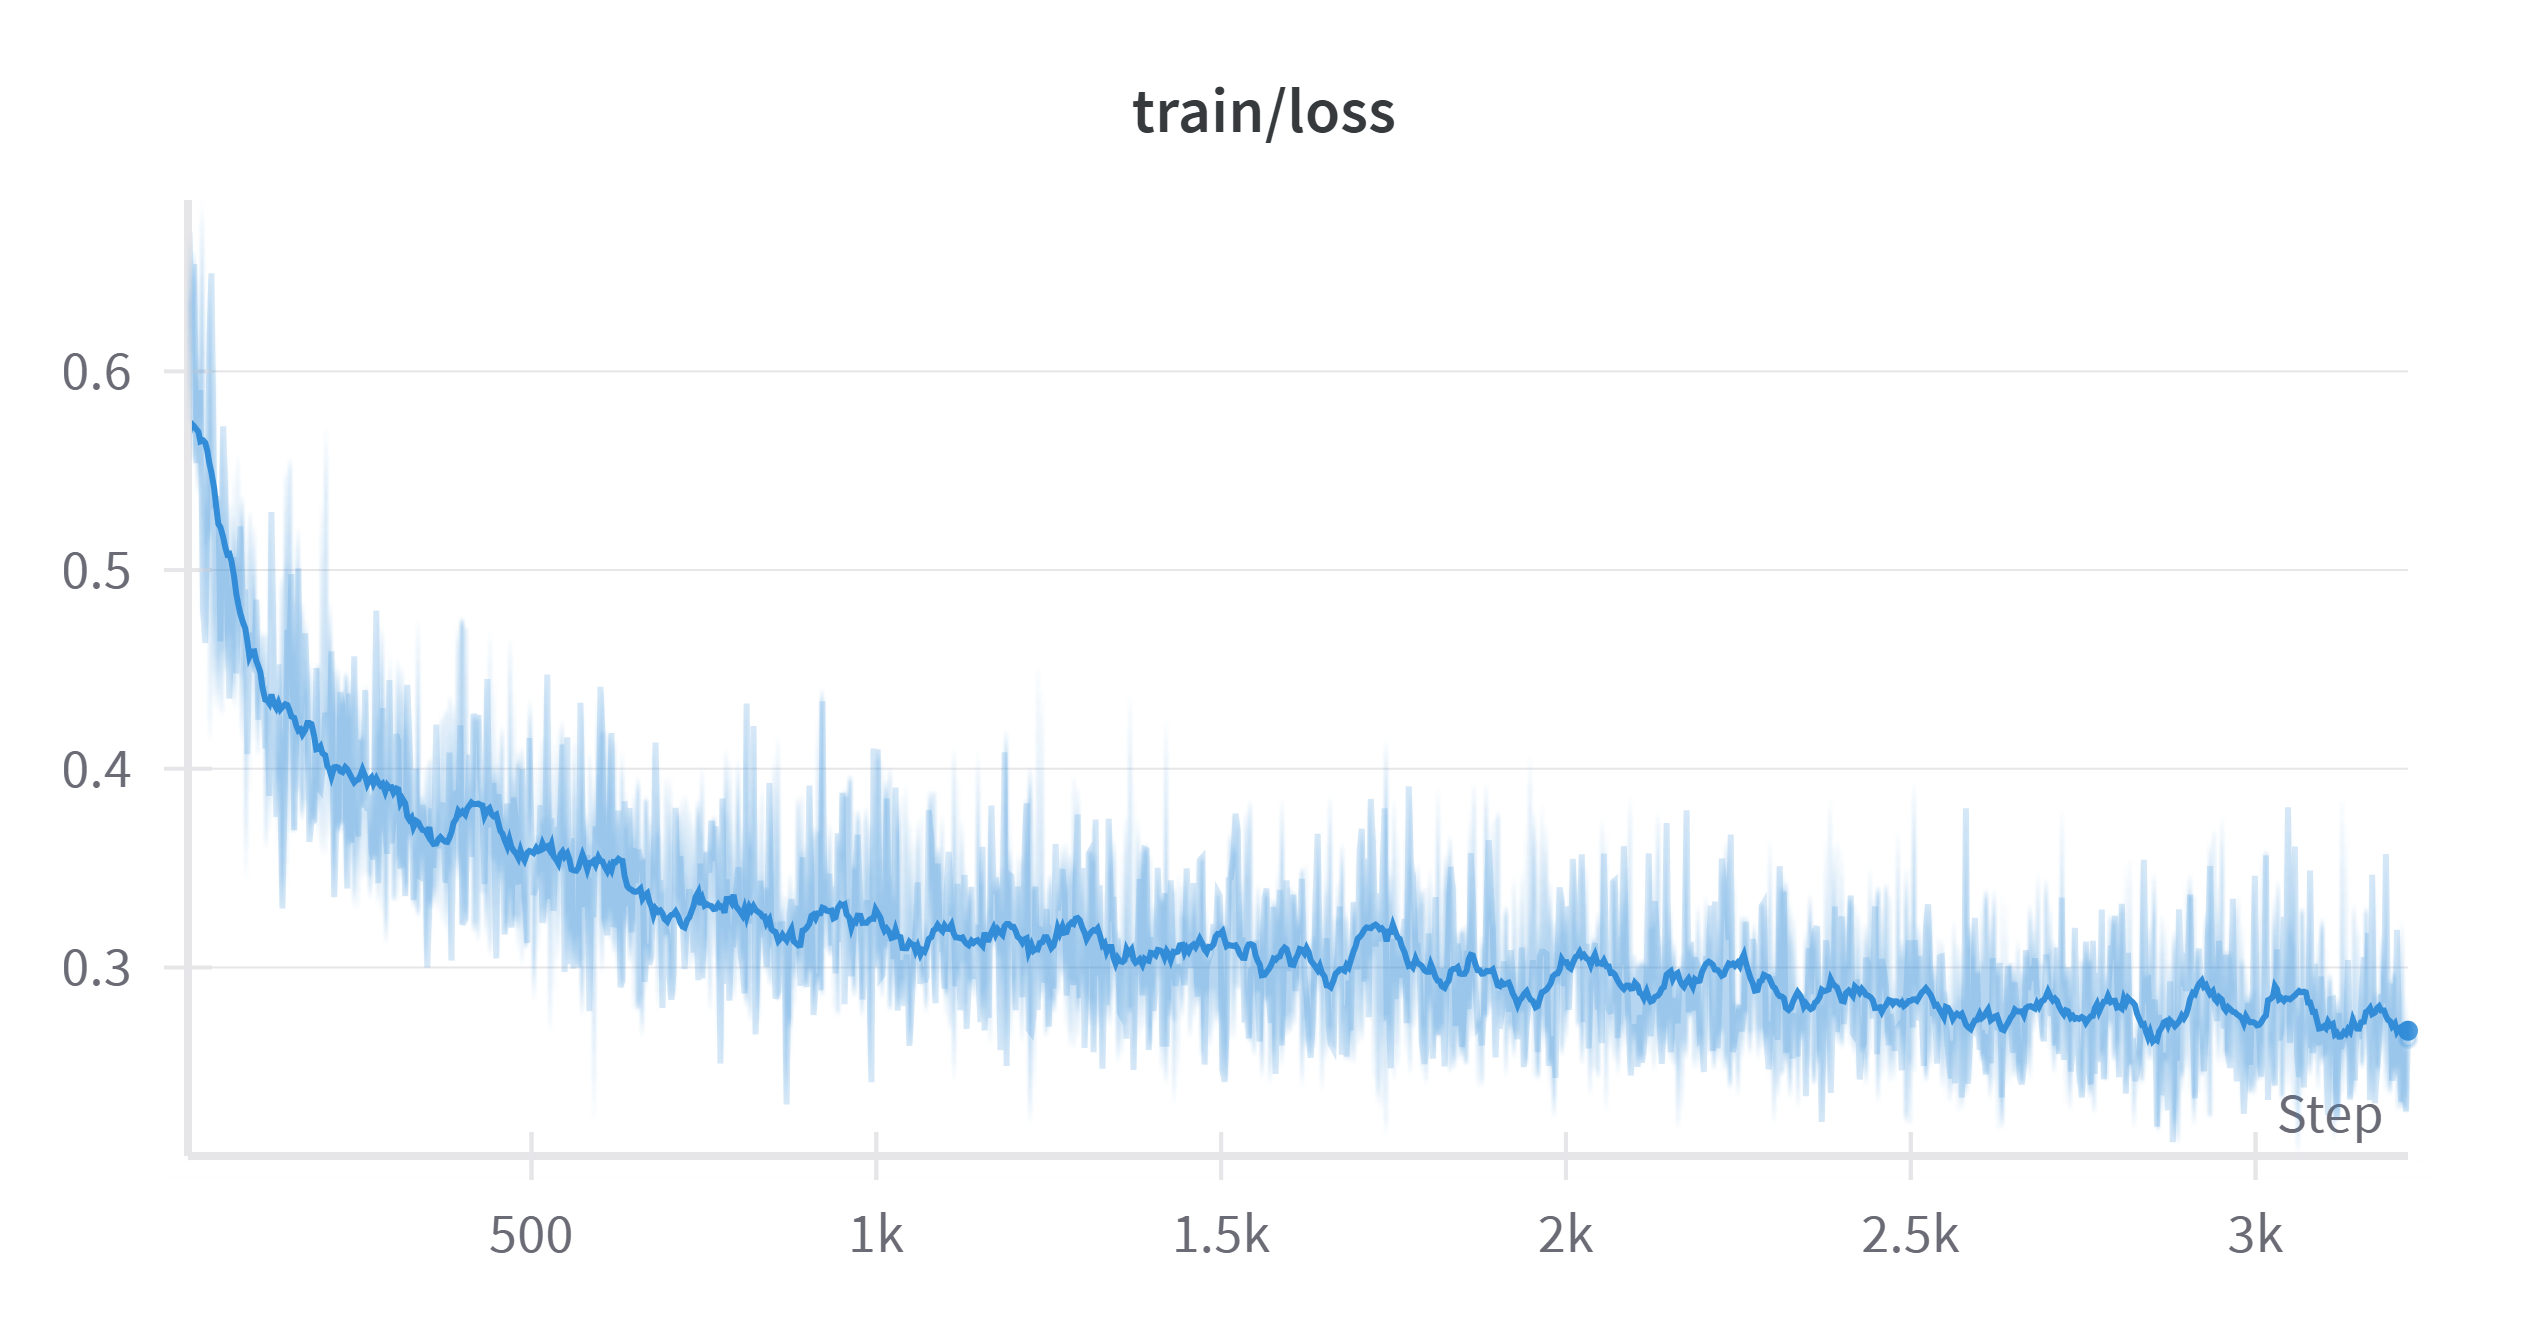
\includegraphics[width=\linewidth]{M2 Course Work/Images/final_training_loss.png}
        \caption{Training Loss} \label{fig:final_training_train_loss}
    \end{subfigure} \hfill
    \begin{subfigure}[b]{0.48\linewidth} \centering
        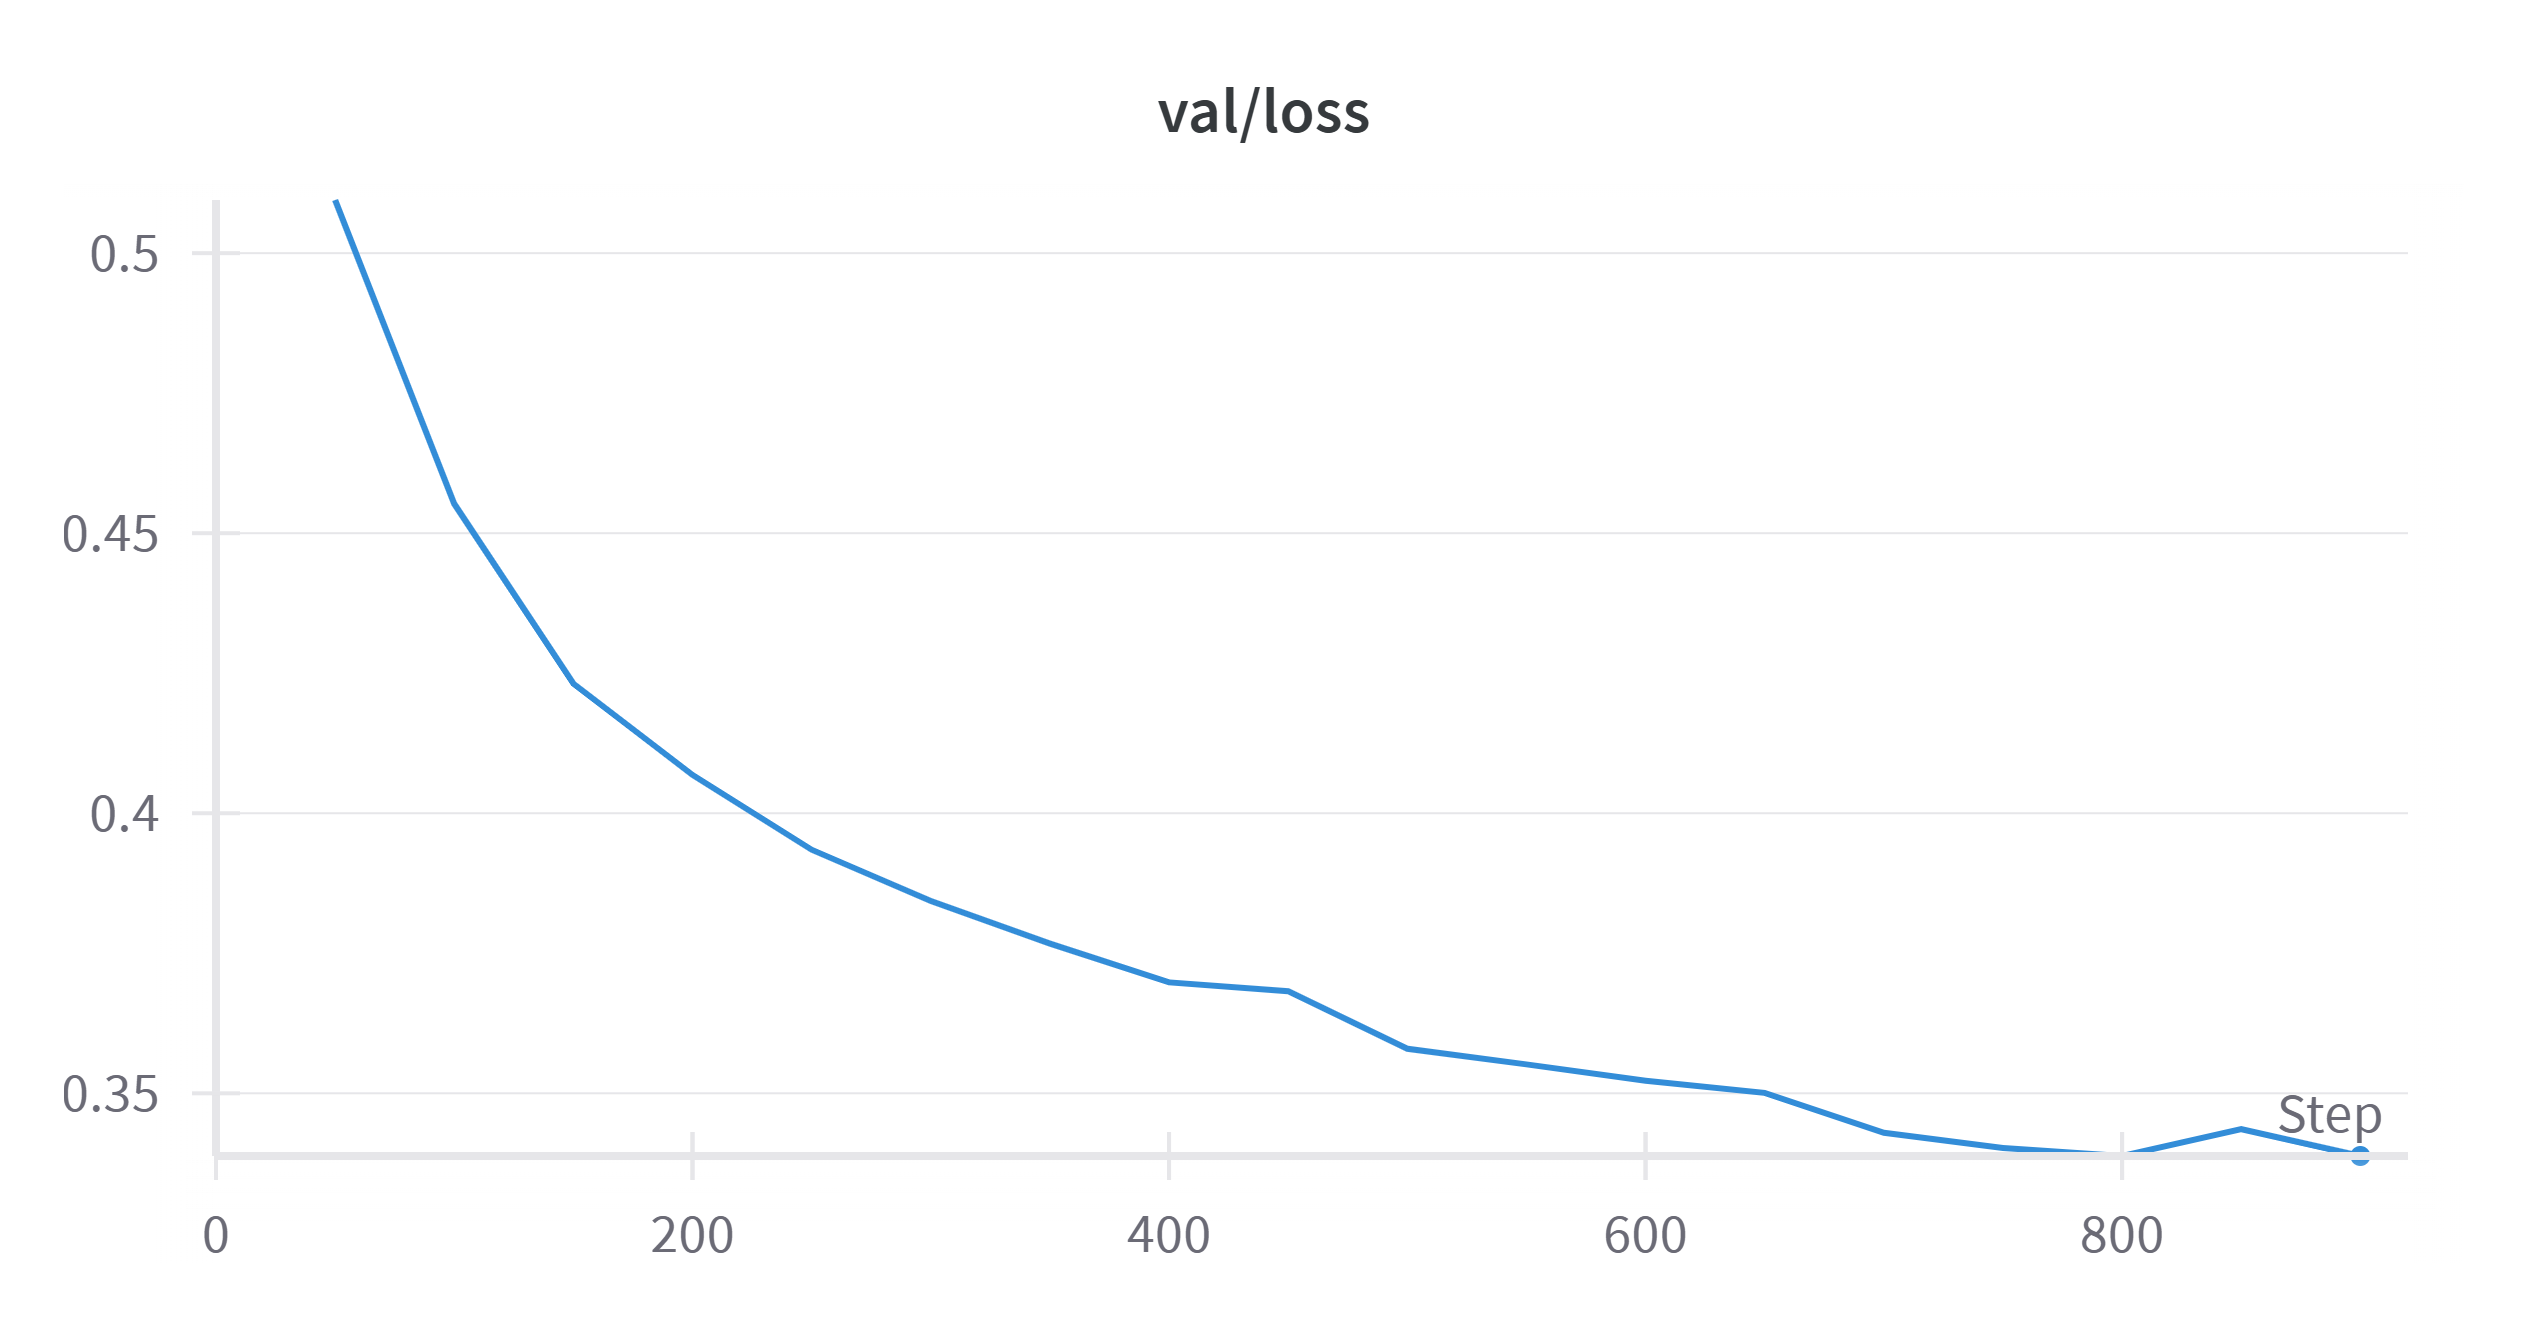
\includegraphics[width=\linewidth]{M2 Course Work/Images/final_validation_loss.png}
        \caption{Validation Loss} \label{fig:final_training_valid_loss}
    \end{subfigure}
    \caption{Loss curves during final training phase ($\eta=10^{-4}, r=8, S=768$).} % Shortened caption
    \label{fig:final_training_loss_curves}
\end{figure}

% Keep Figure: Final Training Predictions

\subsection{FLOPS Usage Summary}
A detailed breakdown of the FLOPS consumed by each experimental run (initial training, grid searches, final training) is provided in Appendix \ref{sec:flops-breakdown}.


\section{Discussion}
\label{sec:discussion}

The experiments demonstrated that \texttt{Qwen-2.5-0.5B-Instruct} can be adapted for time-series forecasting using LoRA with LLMTime. Analysis of model components and limitations reveals further insights.

\paragraph{LM Head Bias Adaptation}
In addition to the LoRA matrices, the final LM Head layer's bias parameters (\texttt{model.model. lm\_head.bias}) were also trained. Analysing these adapted biases (Figure \ref{fig:bias_analysis}) reveals an interesting pattern related to the task structure. While the vast majority of the 151,936 bias values remained negative or zero (Median Bias: -0.0005), precisely seven developed a small positive bias. These correspond to the tokens essential for constructing the LLMTime numerical format ($X.XX,Y.YY;...$, Section \ref{sec:preprocessing}): the structural punctuation \texttt{.}, \texttt{,}, \texttt{;}, and intriguingly, only the digits `0', `2', `7', and `9'. Other digit tokens did not develop a positive bias.


This selective positive biasing of only four digits, which are somewhat evenly spread across the 0-9 range, is noteworthy as an efficient adaptation strategy. Instead of boosting all digits, the model focuses only on these four. One hypothesis for why this is sufficient involves two complementary aspects: Firstly, these boosted digits might serve as readily available 'anchors' or even direct proxies for nearby digits (e.g., approximating `6' with the positively biased `7' with minimal loss) when generating numerical output. Secondly, by ensuring these anchors are likely, the model may be able to generate other non-boosted digit tokens accurately when needed through learned context and internal state adjustments, without requiring a specific positive bias for every single digit.




% Add the figure code here
\begin{figure}[!htbp]
    \centering
    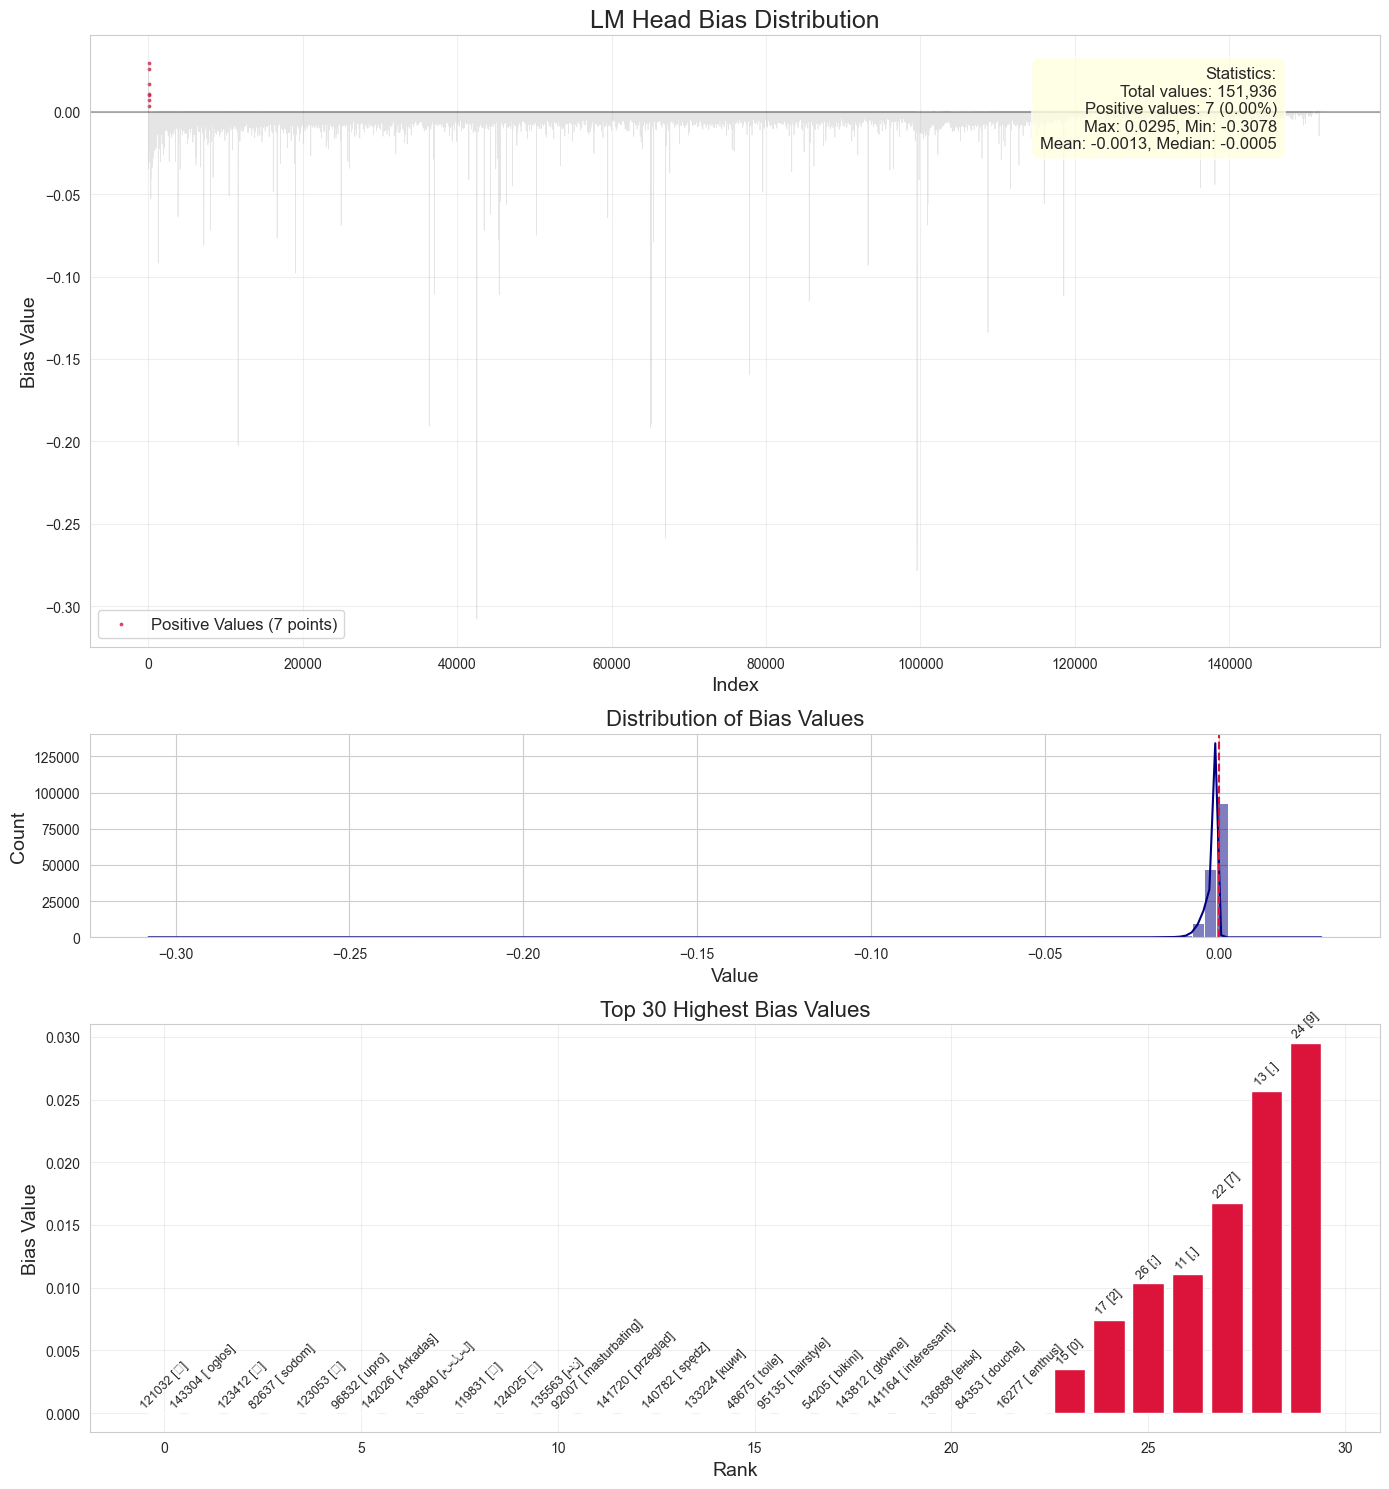
\includegraphics[width=1\linewidth]{M2 Course Work//Images/bias_analysis.png} % Assumed path
    \caption{Analysis of the trainable LM Head bias weights after fine-tuning. Top: Bias values across vocabulary index, highlighting 7 positive values. Middle: Distribution histogram showing concentration below zero. Bottom: Top 30 highest bias values, including the positive ones.}
    \label{fig:bias_analysis}
\end{figure}

\paragraph{Limitations}
Three main limitations impacted this study:
\begin{itemize}
    \item \textbf{Scaling-Induced Prediction Ceiling:} The LLMTime preprocessing scaled data to $[0, 10]$ (Section \ref{sec:preprocessing}). While crucial for token efficiency, this discouraged the model from predicting values exceeding 10, artificially capping or reversing trends during long-term forecasting where true dynamics might surpass this bound (As seen in the third plot of row 1 in Figure \ref{fig:long_term_prediction_failure}, and in detail in Figure \ref{fig:zoomed-up-sequence}). This is an artifact of the how we chose to represent the time-series, not necessarily model learning failure within the scaled range.
    \item \textbf{Data Exclusion from Padding Workaround:} The late discovery of Qwen's left-padding requirement (Section \ref{sec:data-handling}) led us to adopt a workaround by discarding shorter sequence chunks that would have required padding. While this approach ensured correct model behaviour, it resulted in the exclusion of potentially valuable data from the ends of time series during training and evaluation. Fortunately, the lack of tuning for the padding token did not pose a significant drawback when inferring on a single time series.
    \item \textbf{Potential Catastrophic Forgetting:} Intensive fine-tuning for time-series forecasting may have impaired some general abilities. Qualitative tests (Figure \ref{fig:catastrophic_forgetting_analysis}) revealed that the final model misidentified numerical patterns—such as failing to recognize the Fibonacci sequence—and produced flawed explanations of decimal addition, tasks that earlier versions handled correctly. Although basic arithmetic and creative skills remained intact, this degradation suggests that specialization may have led to forgetting, warranting further investigation with larger benchmark datasets like GSM8K \cite{cobbe2021trainingverifierssolvemath} and MATH \cite{hendrycks2021measuringmathematicalproblemsolving}.
\end{itemize}

% Keep Figure: Long Term Prediction Failure
\begin{figure}[!h] % Use htbp
    \centering
    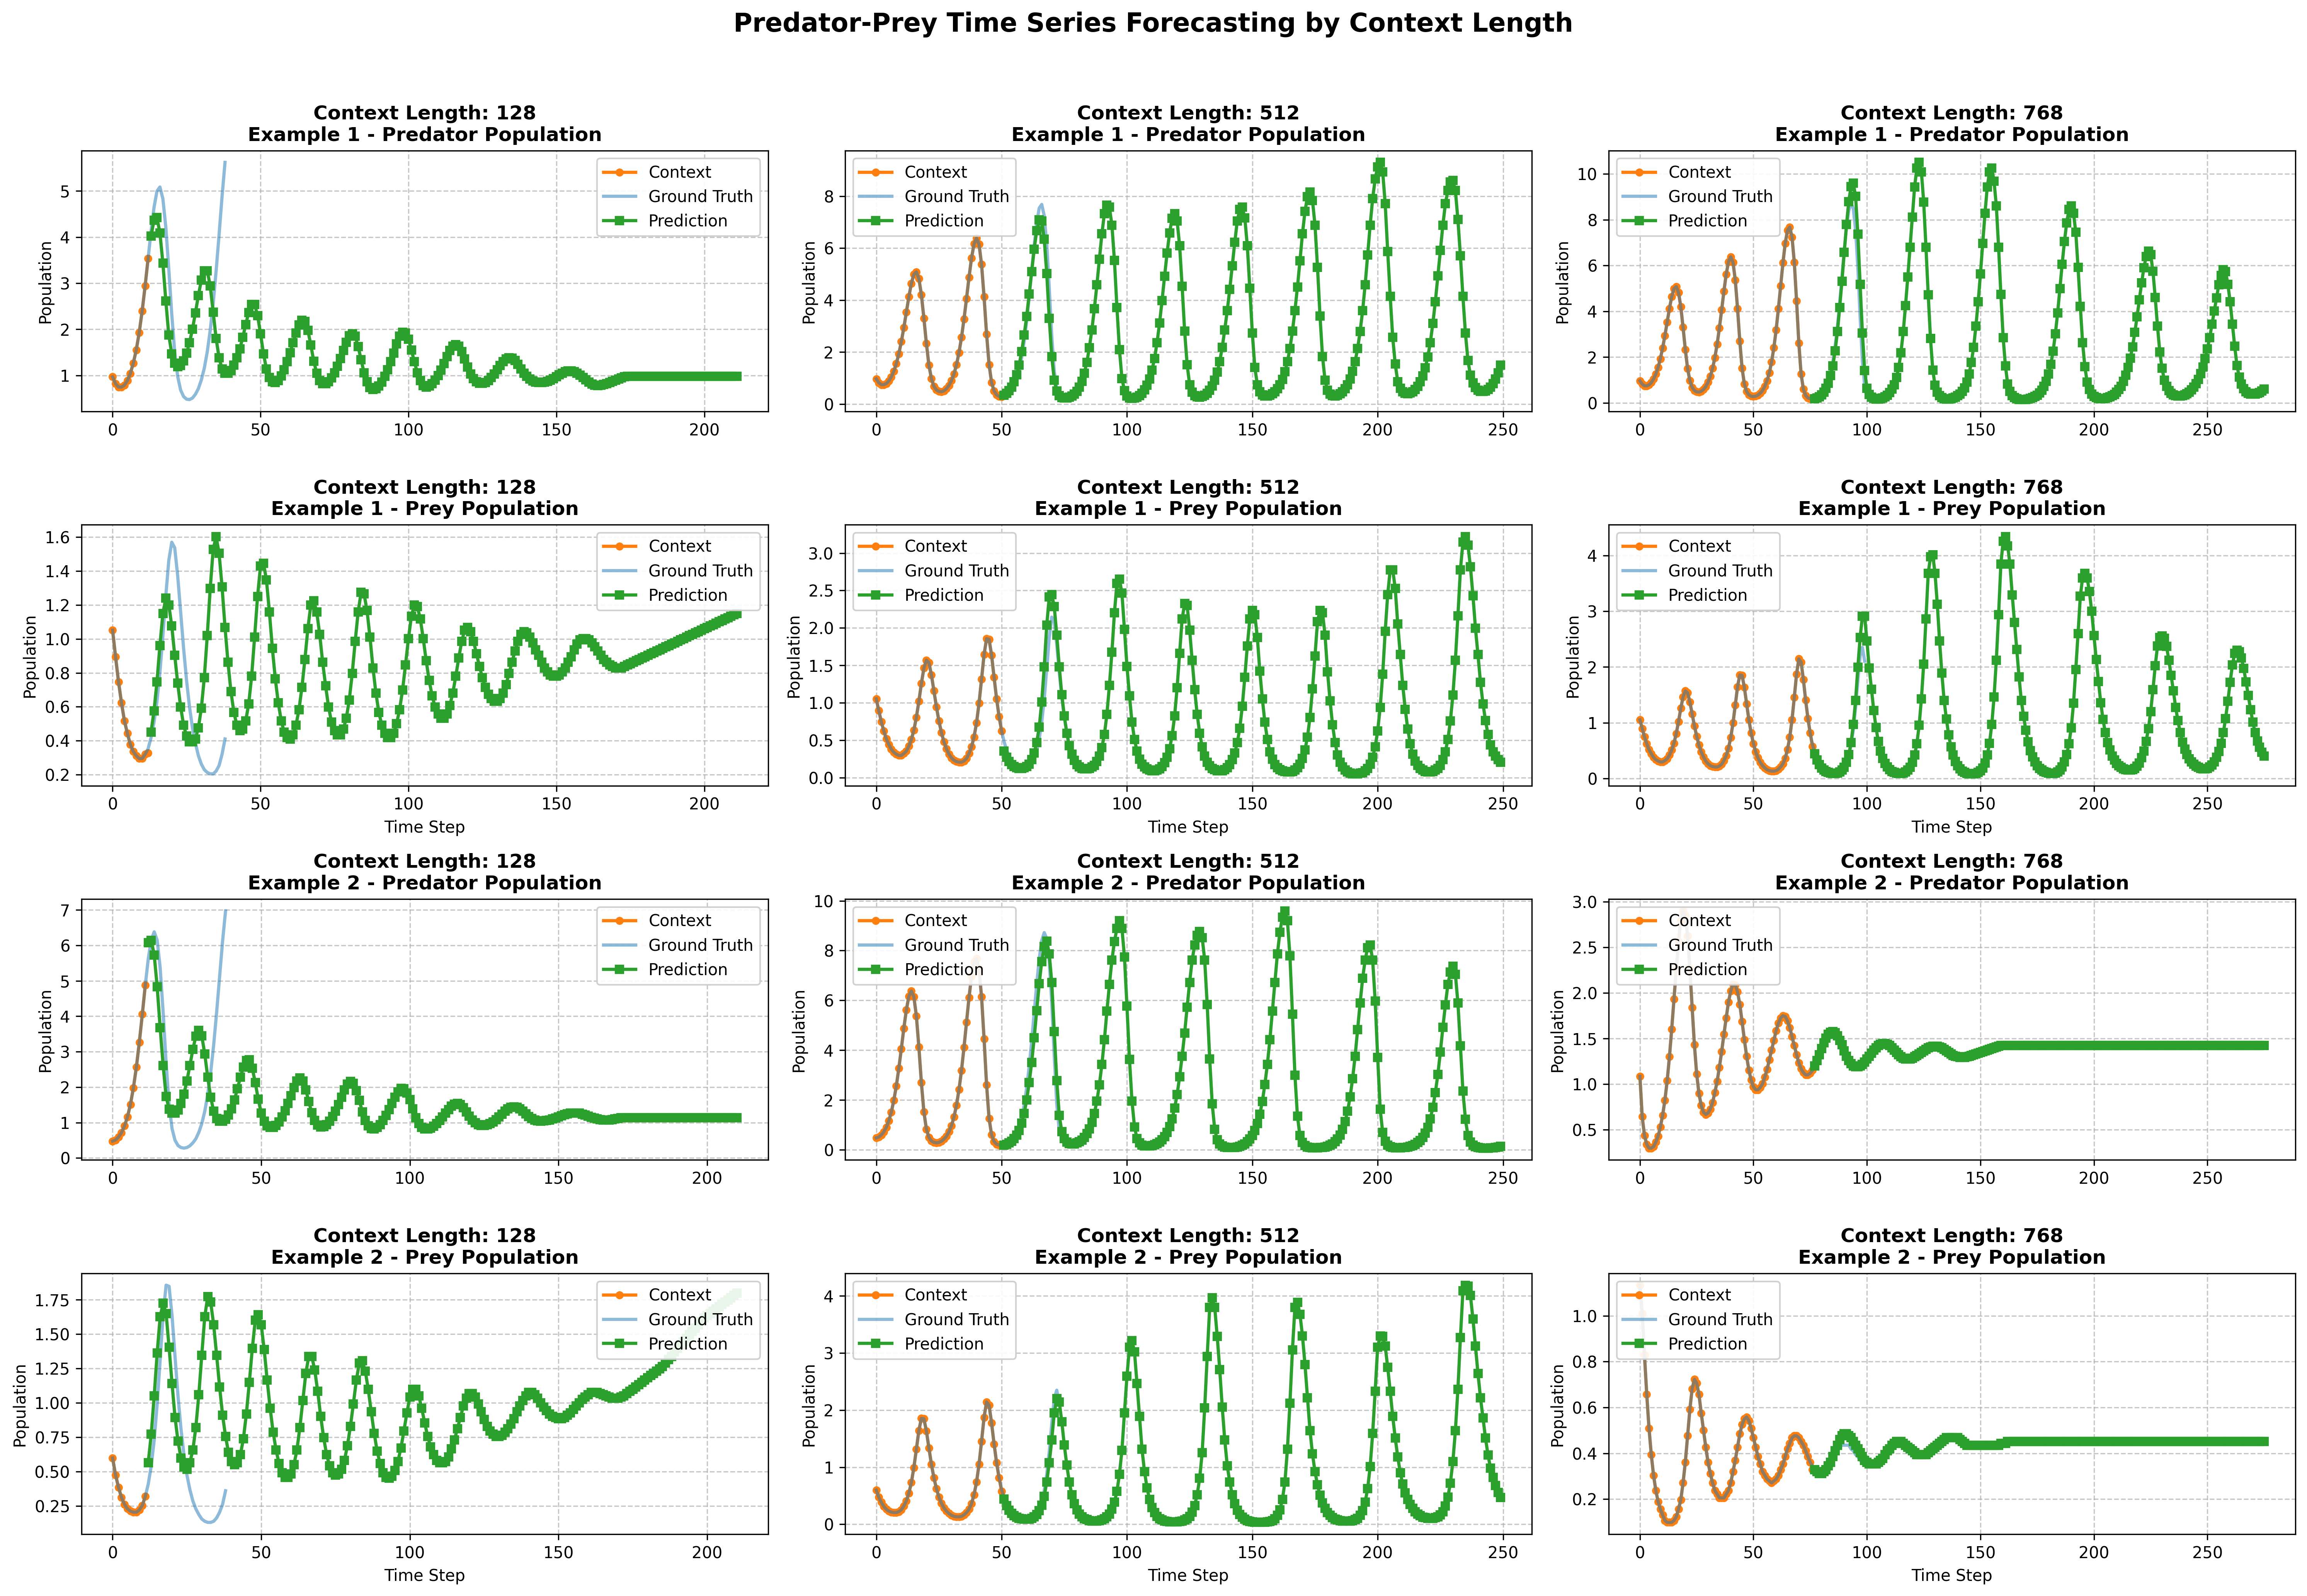
\includegraphics[width=0.8\linewidth]{M2 Course Work//Images/problem_long_sequence.png} % Adjusted width
    \caption{Example of prediction failure during long-term extrapolation (200 time steps). The model (green line) correctly captures the increasing trend initially (see third plot, first row. Figure \ref{fig:zoomed-up-sequence}) but unnaturally reverses direction as the predicted value approaches the normalization ceiling of 10, failing to match the ground truth (blue) which exceeds this bound.}
    \label{fig:long_term_prediction_failure} % Unique label
\end{figure}

\begin{figure}[!htbp]
    \centering
    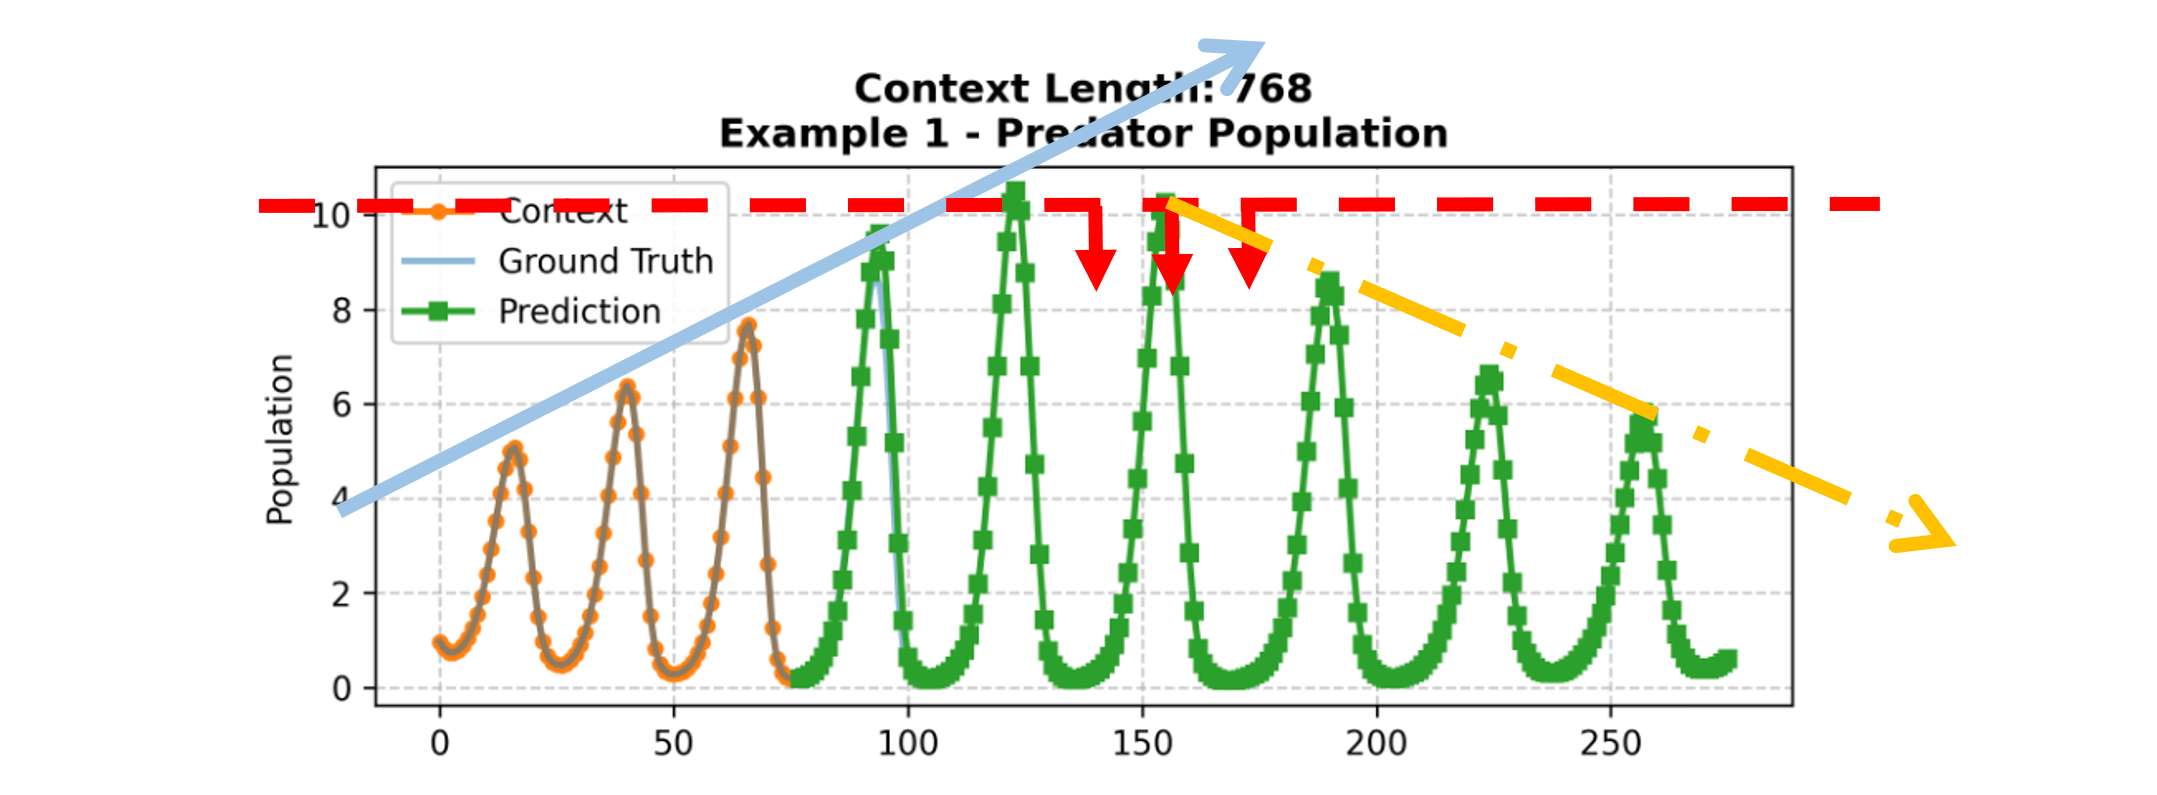
\includegraphics[width=0.75\linewidth]{M2 Course Work//Images/zoomed_up_sequence.png}
    \caption{A zoomed-in view of Figure \ref{fig:long_term_prediction_failure}. The predicted trajectory (green) initially grows, as indicated by the blue arrow. However, once it reaches a population magnitude of 10 (red dashed line), it is suppressed and starts declining, as shown by the red arrows. This suppression leads to an overall downward trend in subsequent oscillations, marked by the yellow dashed arrow.}
    \label{fig:zoomed-up-sequence}
\end{figure}

\begin{figure}
    \centering
    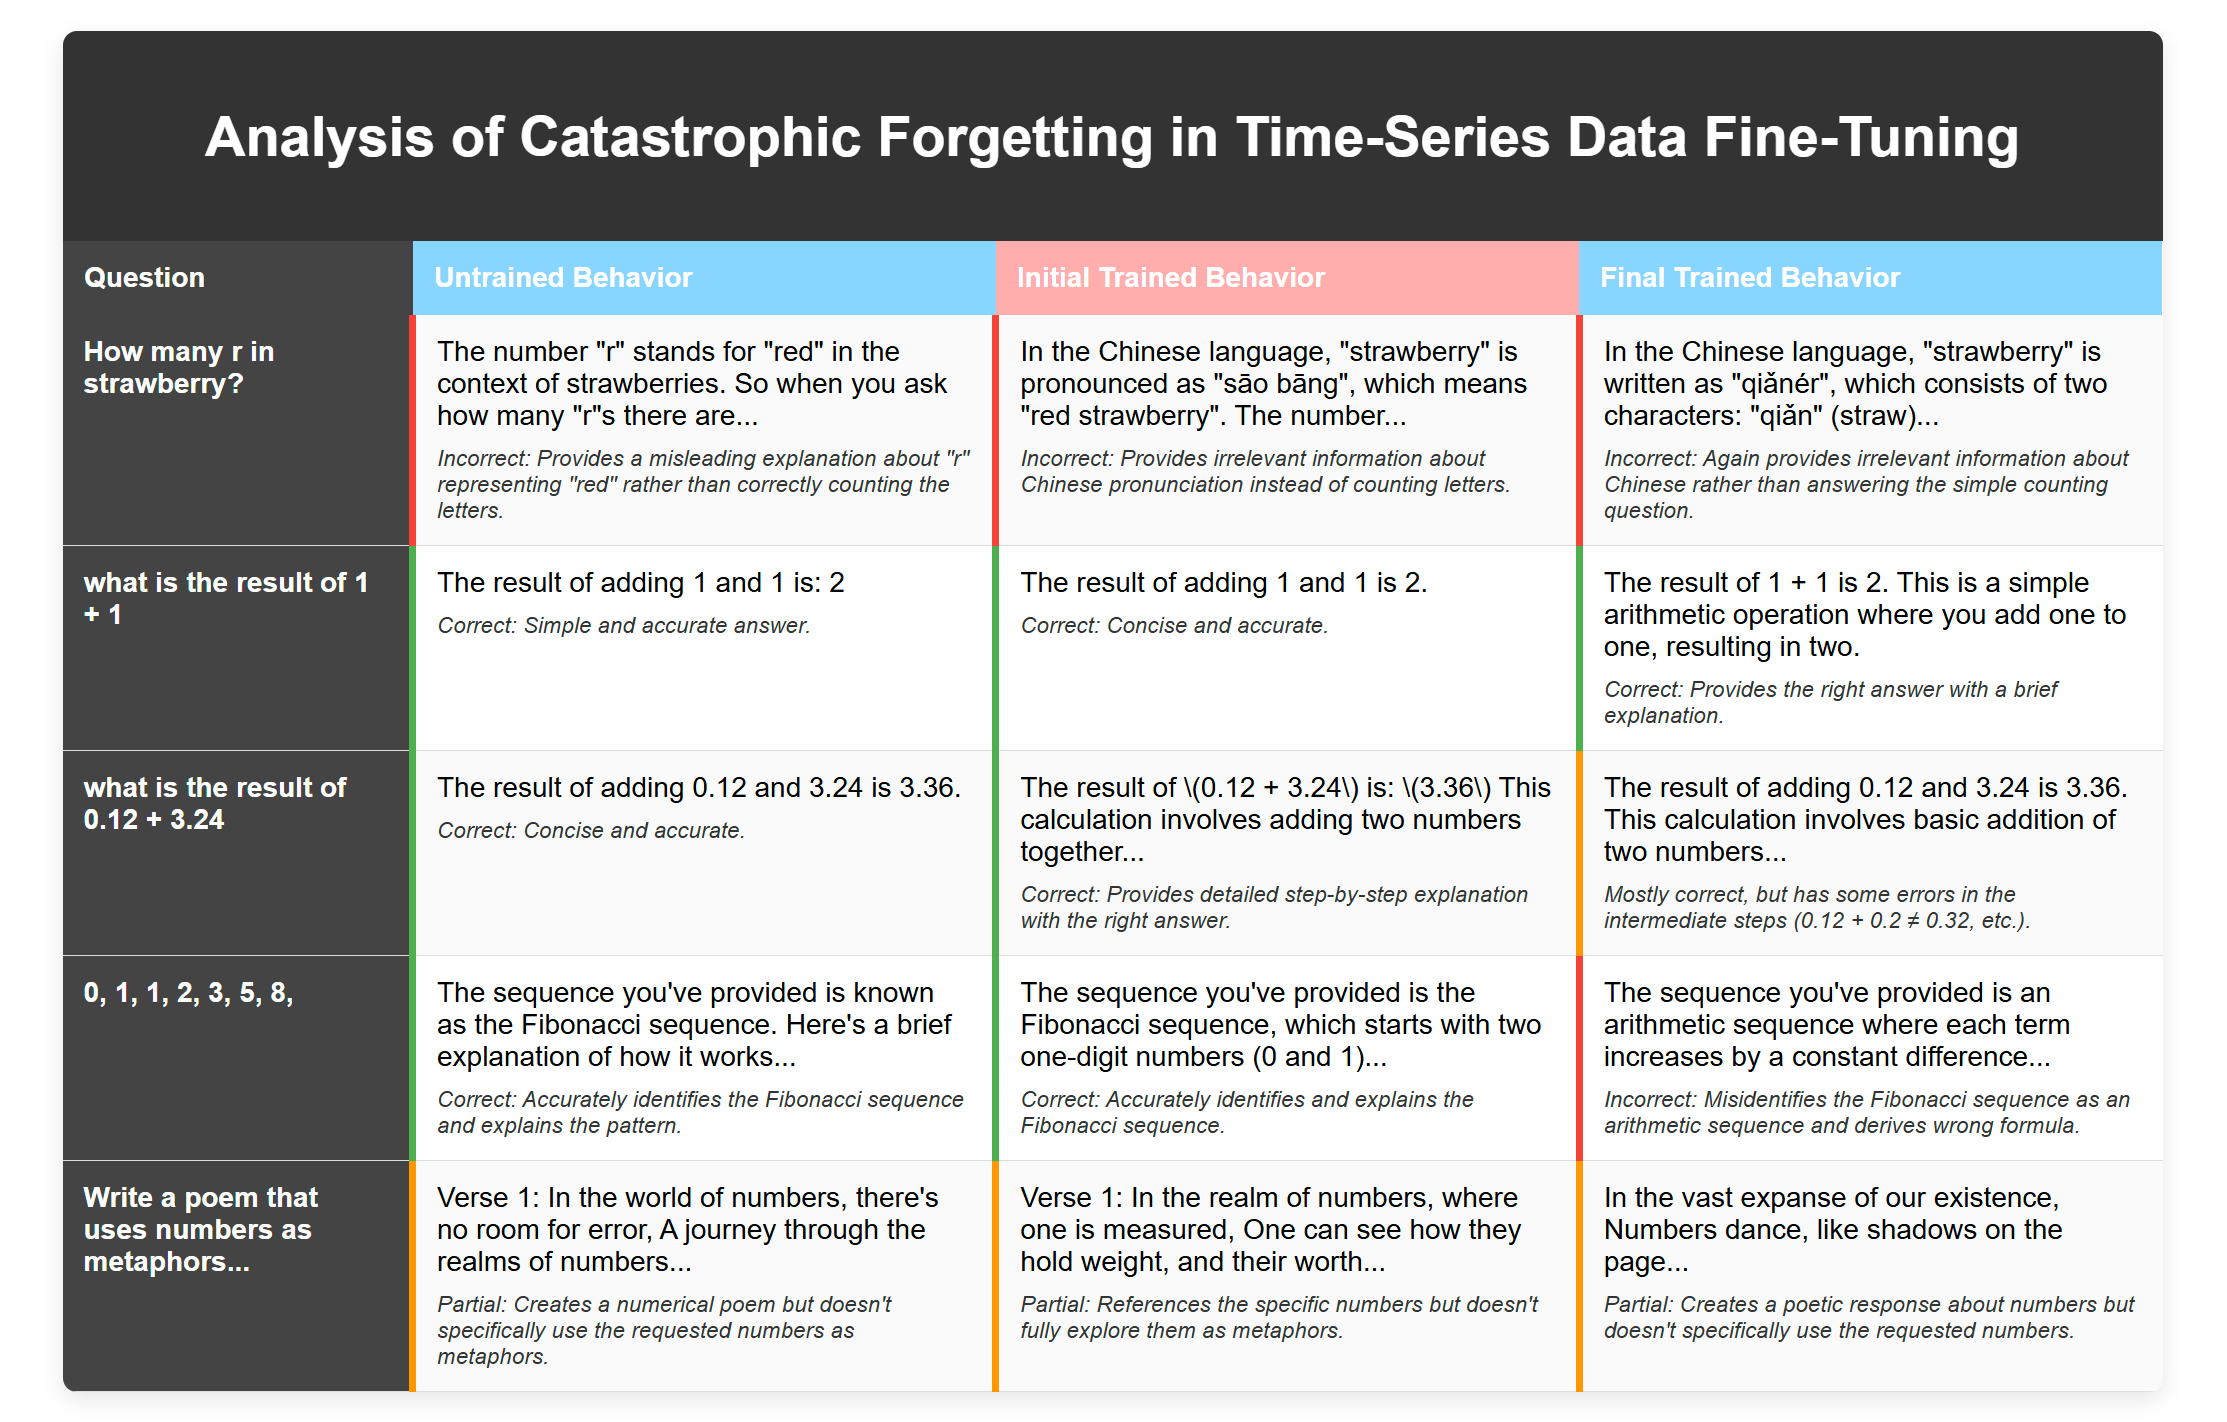
\includegraphics[width=1\linewidth]{M2 Course Work//Images/Catastropic_Forgetting.png}
    \caption{Qualitative analysis of model behavior across training stages on diverse prompts. The final model shows degraded performance on Fibonacci sequence recognition and errors in explaining decimal addition, indicating potential catastrophic forgetting due to specialization.}
\label{fig:catastrophic_forgetting_analysis}
\end{figure}


\paragraph{Recommendations for Budgeted Time-Series Fine-tuning (Q5)}
Based on our experience under the FLOPS constraint:
\begin{itemize}
    \item \textbf{Prioritize Planning:} Accurate FLOPS calculation (Section \ref{sec:flops}) is essential for allocating budget across necessary experimental phases (exploration vs. final training). 
    \item \textbf{Small-Scale Exploration:} Use short runs for hyper-parameter searches before committing significant budget.
    \item \textbf{Small-Scale Data Training:} When data is abundant, using only a fraction of it can be beneficial. However, for this dataset, I experimented with using only 1/10th of the data, but it led to over-fitting too quickly to yield meaningful insights. Therefore, I chose to use the entire dataset.
    \item \textbf{Expect Higher LR/Rank for Domain Shift:} Adapting from language domain to time-series domain might require higher learning rates and LoRA ranks (as seen in Section \ref{sec:results}) than typical LLM fine-tuning to facilitate adaptation.
    \item \textbf{Maximize Context Length:} Longer context lengths consistently improved performance (Section \ref{sec:results});
\end{itemize}

\paragraph{Future Improvements (Q5)}
Potential next steps to enhance performance and efficiency include:
\begin{itemize}
    \item \textbf{Improved Data Handling:} Implement correct left-padding to utilize all data chunks. Investigate alternative numerical representations less prone to clipping, such as xVal which allows continuous numerical tokenization
 \cite{golkar2024xvalcontinuousnumericaltokenization}.
    \item \textbf{Advanced Training Techniques:} use learning rate scheduling (e.g., warmup and decay) for potentially faster adaptation and finer convergence.
    \item \textbf{Efficient LoRA Variants:} Explore methods like dynamic LoRA ranks (e.g., ALoRA \cite{liu2024aloraallocatinglowrankadaptation}, SeLoRA \cite{mao2024seloraselfexpandinglowrankadaptation}) which optimize rank allocation during training. These methods start with a small rank and learn to increase it strategically across different layers, enabling more efficient training, especially in early stages under resource constraints.
    \item \textbf{Quantization:} Apply techniques like QLoRA \cite{dettmers2023qloraefficientfinetuningquantized}, Quantized LoRA, to reduce memory usage and potentially speed up training. Although this doesn't lower FLOPs, it enables training larger models within the same memory budget.
\end{itemize}

\section{Conclusion}
\label{sec:conclusion}
This work demonstrated the adaptation of the \texttt{Qwen-2.5-0.5B-Instruct} LLM for time-series forecasting using LoRA, achieving substantial performance gains within a strict $1 \times 10^{17}$ FLOPS budget. Careful FLOPS planning enabled systematic hyper-parameter optimization, revealing that longer context lengths, higher LoRA ranks, and relatively high learning rates were beneficial for adapting the model from its original language domain. We identified the critical sensitivity of this model to input padding direction (requiring left-padding), a crucial factor for practical application. The optimized model achieved a final MAE of \(0.0191\) (\(S=768\)), representing a sixfold improvement over the untrained model. Despite limitations related to data scaling and a padding workaround, this study confirms the feasibility and effectiveness of fine-tuning tiny LLMs for specialized quantitative tasks under given computational constraints.



\bibliographystyle{plain}
\bibliography{reference}

\appendix



%TC:ignore

\section{AI Usage}
For this report, I declare that Gemini was used to improve grammar, while Claude assisted with coding, specifically in generating more visually appealing plots, partially generating the test suite and README, and providing auto-completion features.

\section{FLOPS Breakdown}
\label{sec:flops-breakdown} 

\begin{table}[!htbp] % Use htbp for better float placement
\renewcommand{\arraystretch}{1.4}
\centering
\sisetup{round-mode=places, round-precision=3} % Ensures consistent decimal places if using siunitx
\setlength{\tabcolsep}{8pt}
% Using siunitx S column for numerical alignment
\begin{tabular}{l S[table-format=2.3]}
    \toprule
    \textbf{Training Phase}           & {\textbf{Budget Usage (\%)}} \\ % Braces needed for header in S column
    \midrule
    Small-scale test (training pipeline validation)                & 0.62349 \\ %
    Initial Training                & 8.000 \\ % Ensure consistent precision
    Grid Search (LR, Rank)        & 36.000 \\
    Sweep over Context Length     & 11.158 \\
    Final Training                  & 40.010 \\
    \midrule % Rule before total
    \textbf{Total Used}             & \bfseries 95.791 \\ % Bold total
    \bottomrule
\end{tabular}
\caption{FLOPS Budget Usage Breakdown by Training Phase, as a percentage of the total $1 \times 10^{17}$ FLOPS budget.} 
\label{tab:flops_budget_usage}
\end{table}

\section{Test Set Prediction Examples} % Changed title slightly for clarity
\label{sec:appendix_predictions} % Added a label for the section

This section provides visual examples of the model's prediction capabilities on test set samples at different training stages.

% Keep Figure: Untrained Predictions
\begin{figure}[!htbp]
    \centering
    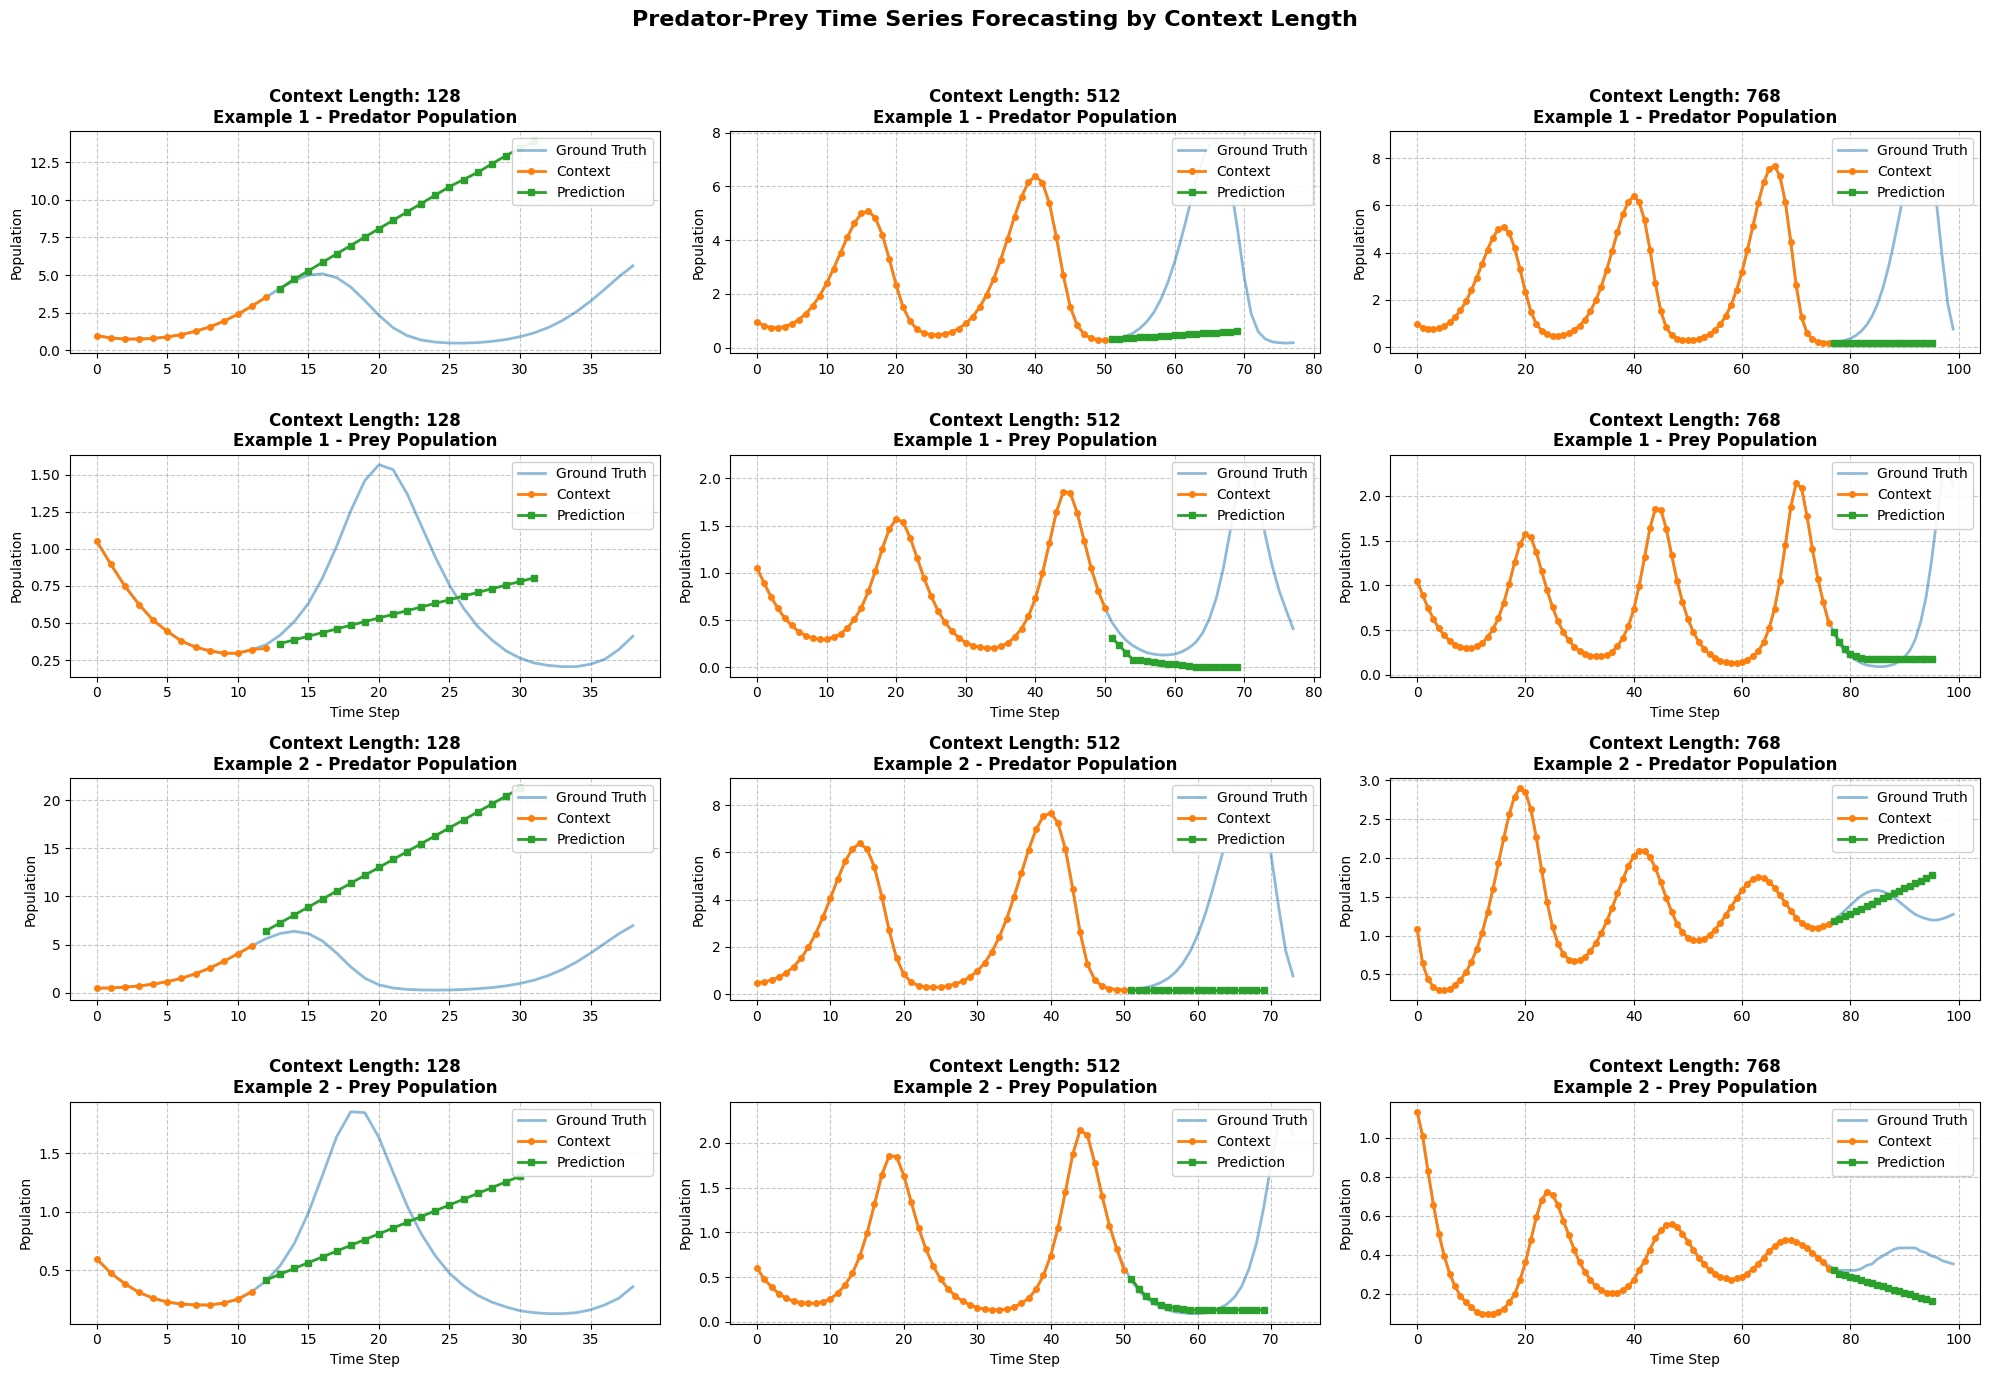
\includegraphics[width=0.9\linewidth]{M2 Course Work//Images/untrained_performance.png}
    \caption{Untrained \texttt{Qwen} predictions (green) vs. ground truth (blue) for 20 steps. The model fails to capture dynamics, predicting near-constant values.} % Shortened caption
    \label{fig:untrained_predictions}
\end{figure}

% Keep Figure: Initial Training Predictions
\begin{figure}[!htbp]
    \centering
    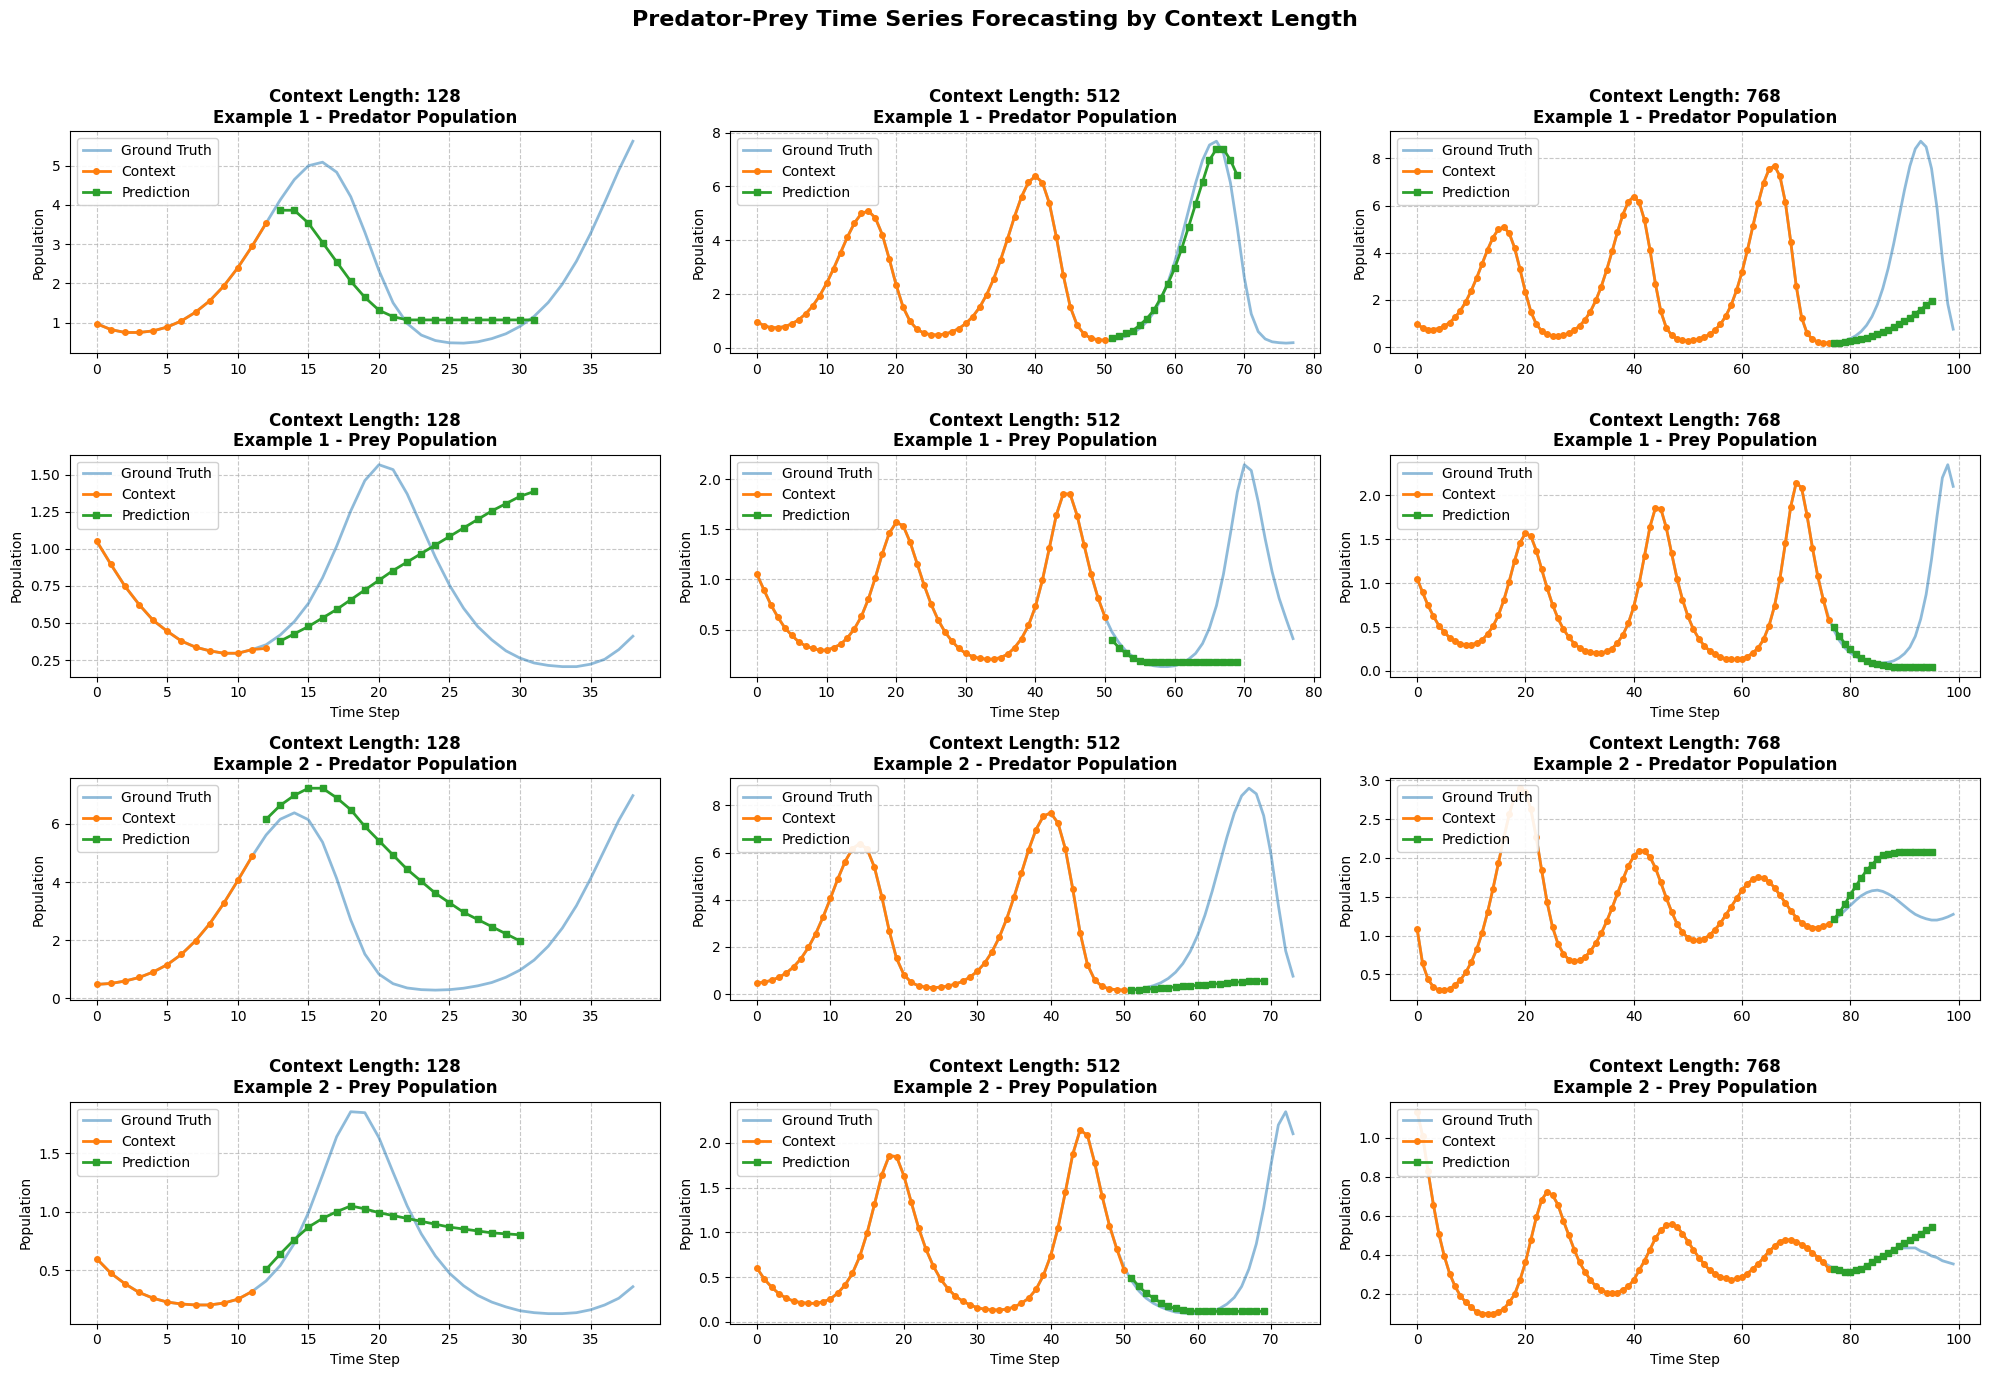
\includegraphics[width=0.9\linewidth]{M2 Course Work//Images/intial_training_result.png}
    \caption{Predictions after initial 1000 training steps. The model now attempts to capture cyclical dynamics, a clear improvement over the untrained state.} % Shortened caption
    \label{fig:initial_training_predictions}
\end{figure}


\begin{figure}[!htbp]
    \centering
    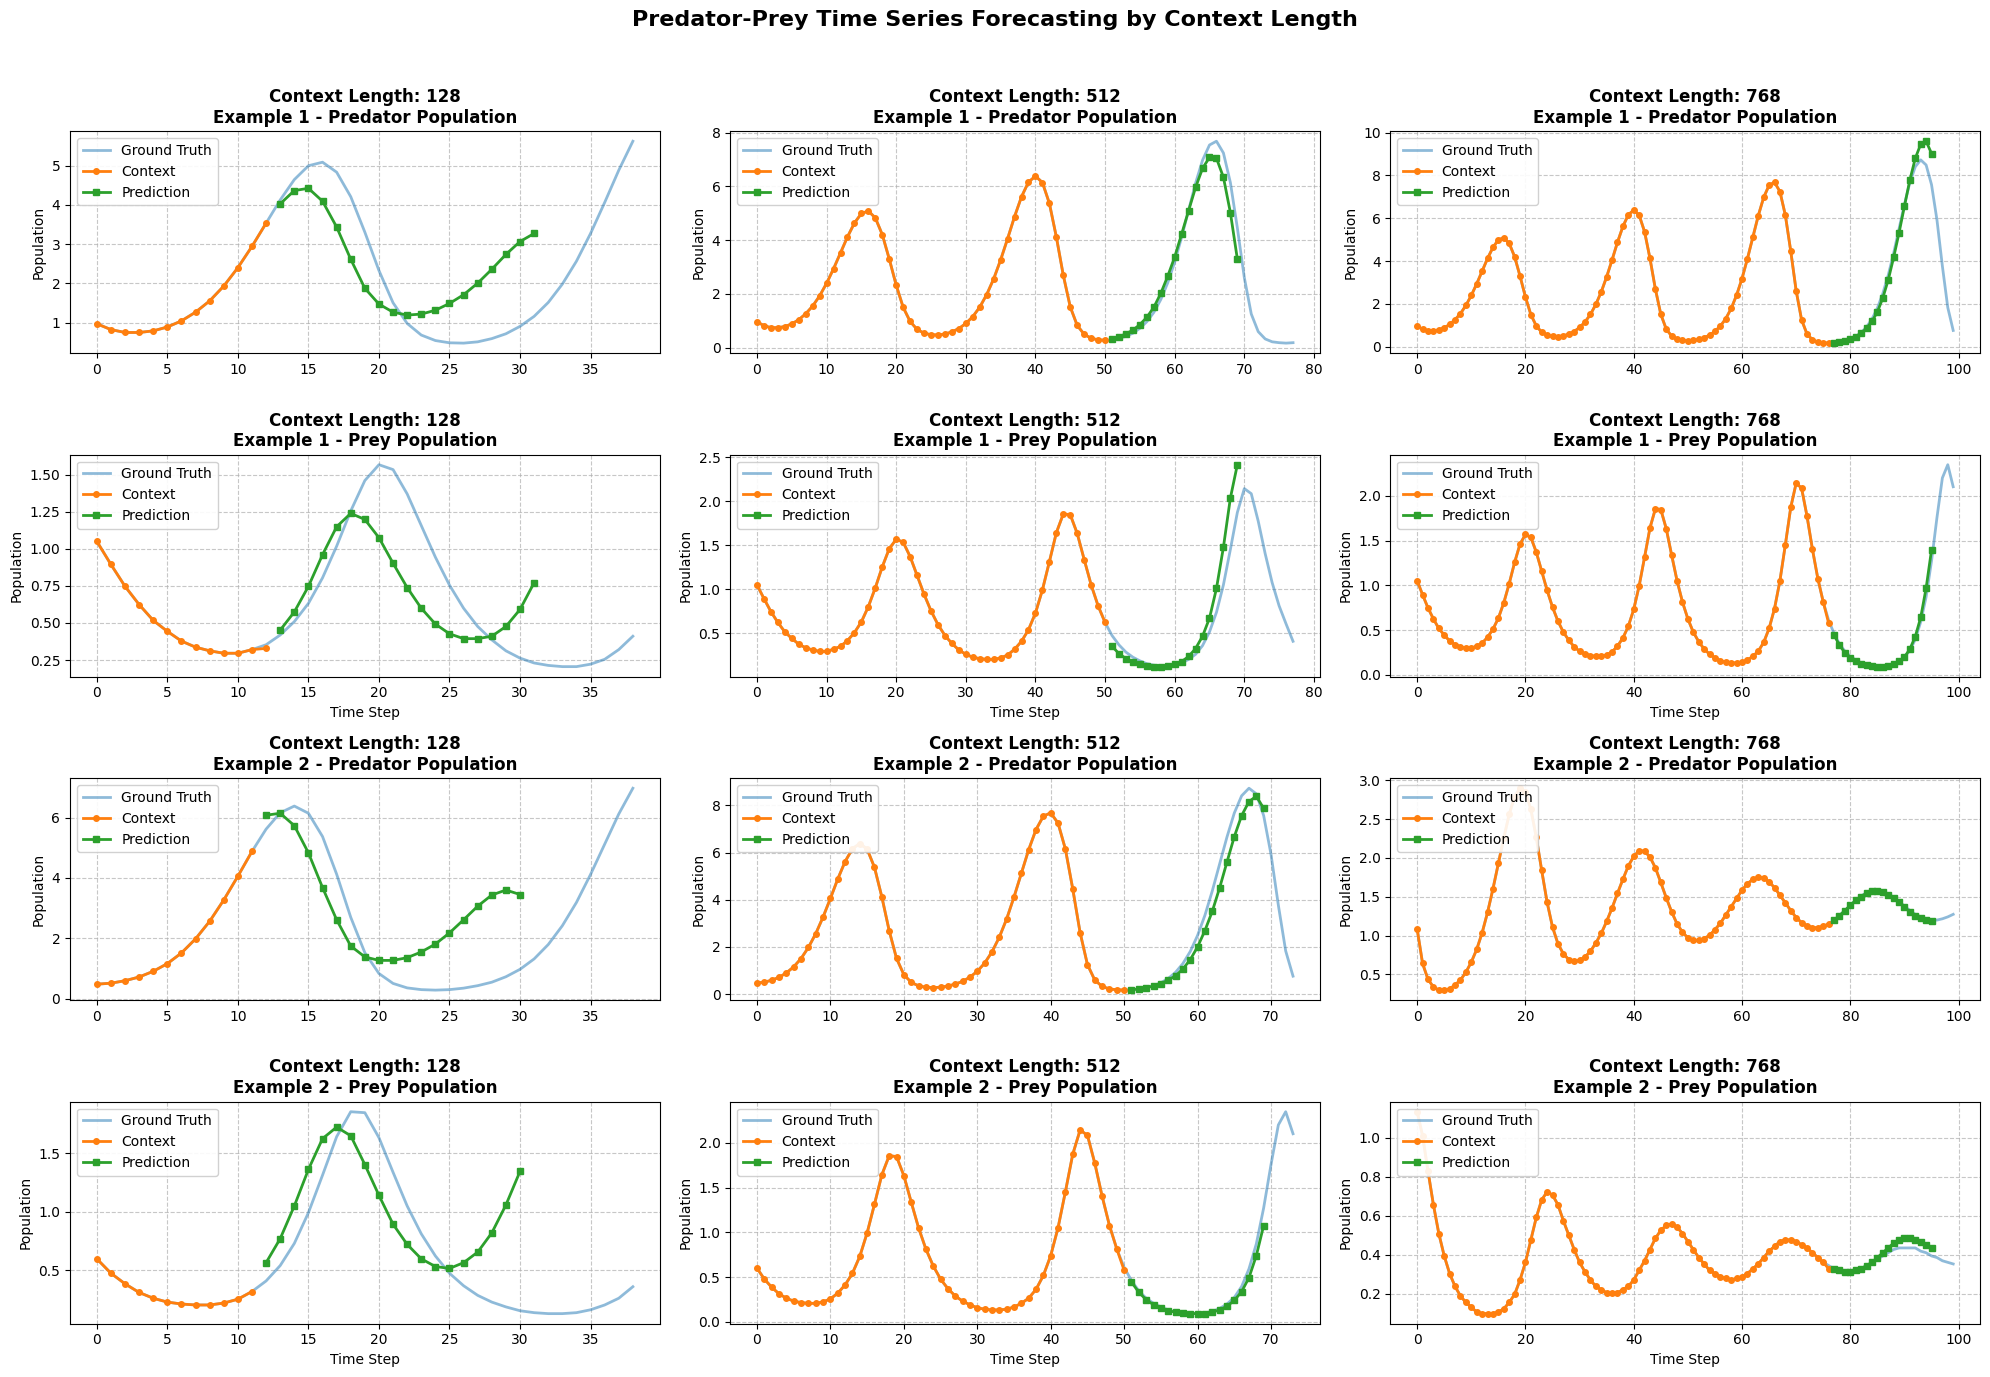
\includegraphics[width=0.8\linewidth]{M2 Course Work//Images/final_training_result.png}
    \caption{Final model predictions. Highly accurate short-term forecasts, especially with longer context ($S=512, 768$).} % Shortened caption
    \label{fig:final_training_predictions}
\end{figure}




\section{Additional LLMTime Samples}

\begin{table}[ht]
  \centering
  \caption{Sample 1 Preprocessing Results}
  \begin{tabular}{>{\bfseries}l l}
    \toprule
    Description & Data \\
    \midrule
    Raw prey data & [0.9714744, 1.0787003, 1.260828, 1.5218158, 1.8605354] \\
    Raw predator data & [1.0054137, 0.82180643, 0.6863802, 0.59312147, 0.53635156] \\
    Tokens  & [16, 13, 17, 18, 11, 16, 13, 17, 22, 26, 16, 13, 18, 21, 11, 16, 13, 15, 19, 26,\\ 
                & \quad 16, 13, 20, 24, 11, 15, 13, 23, 22, 26, 16, 13, 24, 17, 11, 15, 13, 22, 20, 26,\\
                & \quad 17, 13, 18, 20, 11, 15, 13, 21, 23, 26] \\
    \bottomrule
  \end{tabular}
\end{table}

%-------------------------------
% Table for Sample 2
%-------------------------------
\begin{table}[ht]
  \centering
  \caption{Sample 2 Preprocessing Results}
  \begin{tabular}{>{\bfseries}l l}
    \toprule
    Description & Data \\
    \midrule
    Raw prey data & [1.0732226, 0.8540631, 0.7681343, 0.7687197, 0.8349962] \\
    Raw predator data\ & [1.112855, 0.9001321, 0.70823574, 0.55306584, 0.434924] \\
    Tokens & [16, 13, 18, 20, 11, 16, 13, 19, 15, 26, 16, 13, 15, 23, 11, 16, 13, 16, 19, 26,\\ 
                & \quad 15, 13, 24, 22, 11, 15, 13, 23, 24, 26, 15, 13, 24, 22, 11, 15, 13, 22, 15, 26,\\ 
                & \quad 16, 13, 15, 20, 11, 15, 13, 20, 20, 26] \\
    \bottomrule
  \end{tabular}
\end{table}




%TC:endignore

\end{document}